%\section{\centering Experimental Setup}
\chapter{Search for a heavy resonance decaying to a pair of Higgs bosons in the four b quark final state in proton-proton collisions at $\sqrt{s}=13$ TeV}
%\chapter*{\centering Experimental Setup}
\label{ch:Analysis}

The analysis presented in this thesis is the search for a massive resonance decaying into a pair of standard model Higgs bosons in a final state consisting of two b quark-antiquark pairs. The search is performed using a data sample of proton-proton ($pp$) collisions at a center-of-mass energy of 13 TeV collected by the CMS experiment in 2016 and corresponding to an integrated luminosity of $35.9$ $\mathrm{fb}^{-1}$. The Higgs bosons are highly Lorentz-boosted and are each reconstructed as a single large-area jet and identified using jet substructure and b-tagging variables. The signal is characterized by a peak in the dijet invariant mass distribution, above a background from the SM multijet production which is predicted using a data-driven method. The results are consistent with the SM expectations and are interpreted as upper limits on the production cross sections of narrow bulk gravitons and scalar radions in warped extra-dimensional models. 

This chapter first outlines the strategy of the analysis in Section~\ref{sec:Strat}. Then, the datasets and triggers are listed in Sections~\ref{sec:Samples} and~\ref{sec:Triggers}, respectively. In Section~\ref{sec:EvtSel} the event selection is summarized. A full description of the background estimation technique is given in Section~\ref{sec:BkgEst}, followed by the signal modeling in Section~\ref{sec:SignalModel}. Section~\ref{sec:SysUnc} discusses the systematic uncertainties and finally, the results are summarized in Section~\ref{sec:Results}.

\section{Motivation and Strategy}
\label{sec:Strat}

The search for resonant Higgs pair production (HH) is a well motivated BSM search that probes the nature of electroweak symmetry breaking and the possible structure of extra dimensions, as outlined in Section~\ref{sec:HHprod}. Previous searches have been performed by the ATLAS~\cite{ATLAS_HH_GGbb, ATLAS_HH_bbbb, ATLAS_HH_Combined} and CMS~\cite{CMS_HH_bbbb, CMS_HH_tttt, CMS_HH_GGbb, CMS_HH_bbbb2} Collaborations in $pp$ collisions at $\sqrt{s}=7$ and 8 TeV. These searches have included the $bbbb$, $\gamma\gamma bb$, $\tau\tau bb$, and $\gamma\gamma WW^{\ast}$ final states and the $95\%$ confidence level upper limits for the searches done at CMS can be seen in Figure~\ref{fig:HH_8TeV}. There are no significant excesses in these results and up to $m_{X}=1.1$ TeV the WED theory for $\Lambda_R=1$ TeV has been excluded. However, the predicted cross section for $\Lambda_R=3$ TeV is nine times smaller and therefore only limited $m_{X}$ ranges have been excluded by 8 TeV results. With the LHC now running at 13 TeV and collecting a significantly larger amount of data, HH searches can improve their sensitivity, especially at high resonance masses. This is illustrated in the 8 TeV results, where there is an increase in the upper limits for $m_{X} > 2$ TeV, suggesting that the searches have reached the limit of their sensitivity. The four b quark final state is a useful topology to explore the high resonance mass region due to the $H\rightarrow b\bar{b}$ decay having the largest Higgs branching fraction.

\begin{figure}[h!]
  \begin{center}
    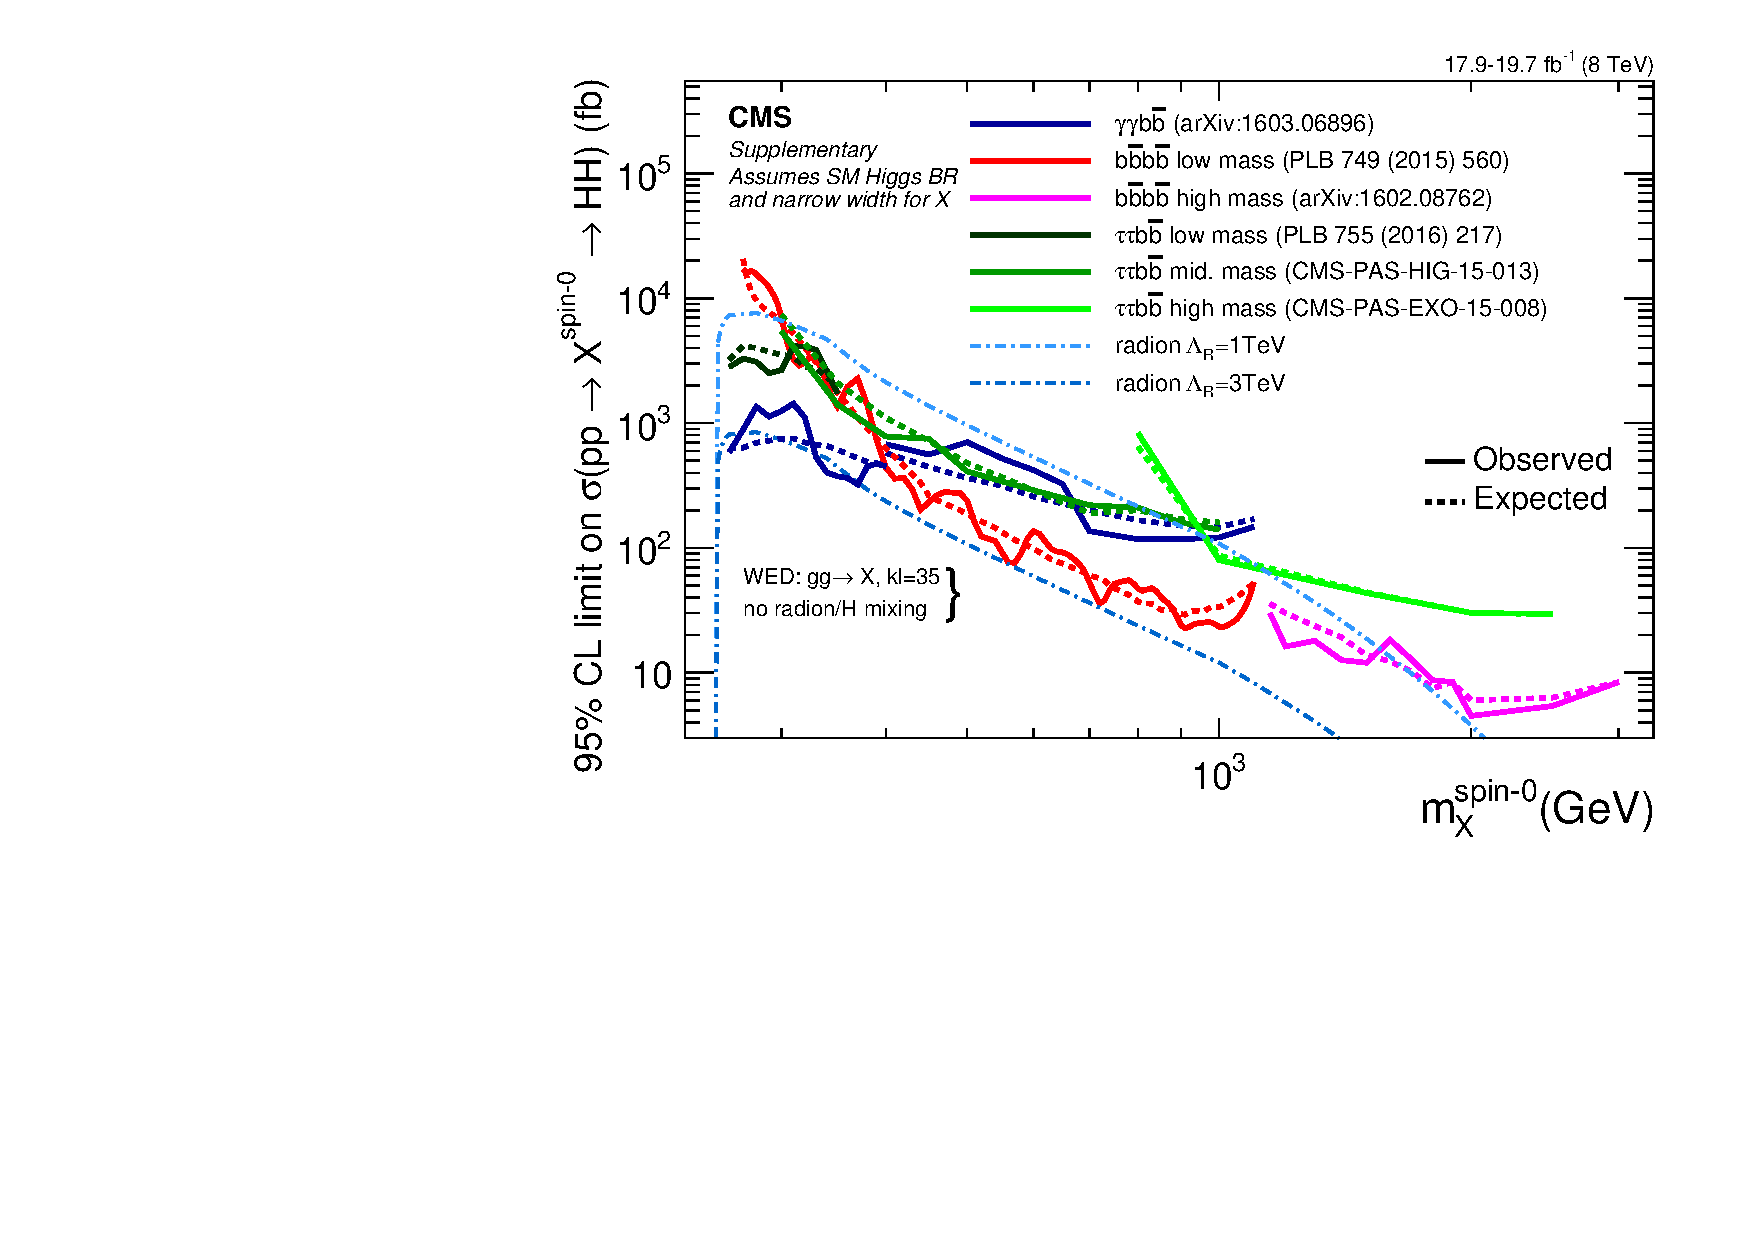
\includegraphics[width=0.8\textwidth]{Analysis/Strategy/Combined_HH_plot_RunI_CMS_spin0.pdf}
  \end{center}
  \caption{Observed and expected $95\%$ confidence level upper limits on the product of the cross section and the branching fraction for the spin-0 radion obtained by different final states explored by the CMS Collaboration at $\sqrt{s}=8$ TeV. Theory lines corresponding to different ultraviolet cutoffs are shown.}
  \label{fig:HH_8TeV}
\end{figure}

%With the LHC now running at 13 TeV, HH searches can improve their sensitivity at high resonance masses. This is illustrated in the 8 TeV results where there is an increase in the upper limits for $m_{X} > 2$ TeV indicating that the searches have reached their sensitivity. The four b quark final state is a useful topology to explore the high resonance mass region due to the $H\rightarrow b\bar{b}$ decay having the largest Higgs branching fraction.


%In searches for Higgs pair production, the four b quark final state is a useful topology to search for due to the $H\rightarrow b\bar{b}$ decay having the largest Higgs branching fraction. This allows the search to look for higher mass resonances than other final states due to the lack of events for these other final states. However, there is a large background from SM multijet production that will have to be dealt with. 

The strategy of this HH analysis is to search for both Higgs bosons decaying through the $H\rightarrow b\bar{b}$ channel, where the final state topology is constrained by $m_{X}/2m_{H}\gg 1$. This requirement forces each Higgs into the boosted regime, which is defined when the Higgs has large momentum so that its decay products are collimated along its direction of motion and is characterized by $\Delta R \sim 2m/p_{T}$, where $m$ and $p_{T}$ are the mass and transverse momentum of the Higgs and $\Delta R$ is the angular separation between the two decay products. The hadronization of a narrowly separated $b\bar{b}$ pair arising from a Higgs boson decay will result in a single reconstructed jet, called a Higgs jet, of mass compatible with $m_{H}$. The Higgs candidates are selected by employing the jet-grooming algorithm called soft-drop mass~\cite{JetMass, SoftDrop}, a jet substructure variable called N-subjettiness~\cite{BoostNsub, BoostTop}, and a double-b tagger~\cite{DoubleB}. The full Higgs jet selection will be given in Section~\ref{sec:EvtSel}.

The background consists mostly of SM multijet production, also called QCD, and is estimated using a fully data-driven technique that uses several control regions defined in the phase space of the mass and double-b tagging discriminator of the leading $p_{T}$ Higgs jet. The background is predicted as a function of dijet invariant mass allowing the entire range of $m_{X}$ to be explored. The signal would appear as a peak in the HH invariant mass spectrum above a smooth background distribution. The complete background estimation technique will be described in more detail in Section~\ref{sec:BkgEst}.

\section{Data and Simulated Samples}
\label{sec:Samples}

The analysis presented in this thesis is performed using $35.9$ $\mathrm{fb}^{-1}$ of $pp$ collision data at $\sqrt{s}=13$ TeV collected with the CMS detector in 2016. Table~\ref{tab:data} lists all of the datasets used and their integrated luminosities.

{\begin{table}[htb]
\renewcommand{\arraystretch}{1.2}
  \begin{center}
    \begin{tabular}{l|c|c}
      \hline
      \hline
      Dataset & Processing & Int. lumi. (fb$^{-1}$) \\
      \hline
      /JetHT/Run2016B   & 03Feb2017 & 5.9  \\
      /JetHT/Run2016C   & 03Feb2017 & 2.6  \\
      /JetHT/Run2016D   & 03Feb2017 & 4.4  \\
      /JetHT/Run2016E   & 03Feb2017 & 4.1  \\
      /JetHT/Run2016F   & 03Feb2017 & 3.2  \\
      /JetHT/Run2016G   & 03Feb2017 & 7.7  \\
      /JetHT/Run2016H   & 03Feb2017 & 8.9 \\
      %JetHT/Run2016B   & 23Sep2016 & 5.9  \\
      %JetHT/Run2016C   & 23Sep2016 & 2.6  \\
      %JetHT/Run2016D   & 23Sep2016 & 4.4  \\
      %JetHT/Run2016E   & 23Sep2016 & 4.1  \\
      %JetHT/Run2016F   & 23Sep2016 & 3.2  \\
      %JetHT/Run2016G   & 23Sep2016 & 7.7  \\
      %JetHT/Run2016H   & PromptReco & 8.9 \\
      \hline
      Total & & 35.9 \\
      \hline
      \hline
    \end{tabular}
  \end{center}
 \caption{List of the primary datasets, their data reconstruction campaign, and their corresponding integrated luminosity. The different datasets correspond to different detector and trigger configurations used by CMS.\label{tab:data}}
\end{table}}

The Monte Carlo (MC) signal samples used in this analysis are listed in Table~\ref{tab:signal_MC}. They include spin-0 bulk gravitons and spin-2 radions produced via gluon-gluon fusion and simulated to leading order (LO) in QCD precision. The samples decay to the four b quark final state and the mass of the resonances range between $750-3000$ GeV with a width of 1 MeV, corresponding to the narrow width approximation. The primary versions of these samples are simulated using the \textsc{madgraph5}$\_$a\textsc{mc}\textsc{@nlo}2.3.3~\cite{MADGRAPH} event generator with the NNPDF3.0 leading order parton distribution functions (PDFs)~\cite{PDFs} taken from the LHAPDF6 PDF set~\cite{PDF2, PDF3, PDF4, PDF5}. The showering and hadronization of partons is simulated with \textsc{pythia} 8.212~\cite{Pythia} with the CUETP8M1-NNPDF23LO~\cite{CUET} tune. The alternate version of these samples are generated with \textsc{herwig++} 2.7.1 and are used to evaluate the systematic uncertainty associated with the parton shower and hadronization which will be described in Section~\ref{sec:SysUnc}. These samples use the EE5C tune~\cite{EE5C}.

%\begin{table}[h!]
 % \begin{center}
 %   \begin{tabular}{l|c|c}
 %     \hline
 %     \hline
 %     \multicolumn{3}{c}{Bulk graviton} \\ \cline{1-3}
 %     Process & $\sigma$ (pb) (LO) & Events\\ \hline
 %     \hline
 %     {GluGluToBulkGravitonToHHTo4B_\M-750\_narrow\_13TeV-madgraph} & 2.66 &99200 \\
 %     {GluGluToBulkGravitonToHHTo4B_\M-800\_narrow\_13TeV-madgraph} & 2.66 &100000 \\
 %     {GluGluToBulkGravitonToHHTo4B_\M-900\_narrow\_13TeV-madgraph} & 2.66 &100000 \\
 %     {BulkGravTohhTohbbhbb\_narrow\_M-1000\_13TeV-madgraph} & 0.08079 &50000 \\
%      {BulkGravTohhTohbbhbb\_narrow\_M-1200\_13TeV-madgraph} & 0.03629 & 50000 \\
%      {BulkGravTohhTohbbhbb\_narrow\_M-1400\_13TeV-madgraph} & 0.0173 & 50000 \\
%      {BulkGravTohhTohbbhbb\_narrow\_M-1600\_13TeV-madgraph} & 0.00867 & 50000 \\
%      {BulkGravTohhTohbbhbb\_narrow\_M-1800\_13TeV-madgraph} & 0.004513 & 48400 \\
%      {BulkGravTohhTohbbhbb\_narrow\_M-2000\_13TeV-madgraph} & 0.002426 & 50000 \\
%      {BulkGravTohhTohbbhbb\_narrow\_M-2500\_13TeV-madgraph} & 0.0005651 & 50000 \\
%      {BulkGravTohhTohbbhbb\_narrow\_M-3000\_13TeV-madgraph} & 0.000144 & 50000 \\
%      \hline
%      \multicolumn{3}{c}{Bulk graviton \texttt{Herwig++ samples}} \\ \cline{1-3}
%      {BulkGravTohhTohbbhbb\_narrow\_M-1000\_13TeV-madgraph-herwig} & 0.08079  & 50000 \\
%      {BulkGravTohhTohbbhbb\_narrow\_M-2000\_13TeV-madgraph-herwig} & 0.002426 & 50000 \\
%      {BulkGravTohhTohbbhbb\_narrow\_M-3000\_13TeV-madgraph-herwig} & 0.000144 & 50000 \\
%      \hline
%      \multicolumn{3}{c}{Radion} \\ \cline{1-3}
%      \hline
%      {GluGluToRadionToHHTo4B_\M-750\_narrow\_13TeV-madgraph} & 2.66 &99800 \\
%      {GluGluToRadionToHHTo4B_\M-800\_narrow\_13TeV-madgraph} & 2.66 &100000 \\
%      {GluGluToRadionToHHTo4B_\M-900\_narrow\_13TeV-madgraph} & 2.66 &100000 \\
%      {RadionTohhTohbbhbb\_narrow\_M-1000\_13TeV-madgraph} & 1318  & 50000 \\
%      {RadionTohhTohbbhbb\_narrow\_M-1200\_13TeV-madgraph} & 116.2 & 50000 \\
%      {RadionTohhTohbbhbb\_narrow\_M-1400\_13TeV-madgraph} & 67.97 & 50000 \\
%      {RadionTohhTohbbhbb\_narrow\_M-1600\_13TeV-madgraph} & 41.74 & 50000 \\
%      {RadionTohhTohbbhbb\_narrow\_M-1800\_13TeV-madgraph} & 26.57 & 50000 \\
%      {RadionTohhTohbbhbb\_narrow\_M-2000\_13TeV-madgraph} & 17.43 & 50000 \\
%      {RadionTohhTohbbhbb\_narrow\_M-2500\_13TeV-madgraph} & 6.646 & 50000 \\
%      {RadionTohhTohbbhbb\_narrow\_M-3000\_13TeV-madgraph} & 1.519 & 50000 \\
%      \hline
%      \hline
%    \end{tabular}
%  \end{center}
%  \caption{List of Monte Carlo signal samples used. The cross sections and number of events generated are also listed. \label{tab:signal_MC}}
%\end{table}

\begin{table}[h!]
  \begin{center}
    \begin{tabular}{l|c}
      \hline
      \hline
      Process & Events\\ 
      \hline
      \multicolumn{2}{c}{Bulk graviton} \\ \cline{1-2}
      {GluGluToBulkGravitonToHHTo4B\_M-750\_narrow\_13TeV-madgraph}  &99200 \\
      {GluGluToBulkGravitonToHHTo4B\_M-800\_narrow\_13TeV-madgraph}  &100000 \\
      {GluGluToBulkGravitonToHHTo4B\_M-900\_narrow\_13TeV-madgraph}  &100000 \\
      {BulkGravTohhTohbbhbb\_narrow\_M-1000\_13TeV-madgraph}  &50000 \\
      {BulkGravTohhTohbbhbb\_narrow\_M-1200\_13TeV-madgraph}  & 50000 \\
      {BulkGravTohhTohbbhbb\_narrow\_M-1400\_13TeV-madgraph}  & 50000 \\
      {BulkGravTohhTohbbhbb\_narrow\_M-1600\_13TeV-madgraph}  & 50000 \\
      {BulkGravTohhTohbbhbb\_narrow\_M-1800\_13TeV-madgraph}  & 48400 \\
      {BulkGravTohhTohbbhbb\_narrow\_M-2000\_13TeV-madgraph}  & 50000 \\
      {BulkGravTohhTohbbhbb\_narrow\_M-2500\_13TeV-madgraph}  & 50000 \\
      {BulkGravTohhTohbbhbb\_narrow\_M-3000\_13TeV-madgraph}  & 50000 \\
      \hline
      \multicolumn{2}{c}{Bulk graviton \texttt{Herwig++ samples}} \\ \cline{1-2}
      {BulkGravTohhTohbbhbb\_narrow\_M-1000\_13TeV-madgraph-herwig}   & 50000 \\
      {BulkGravTohhTohbbhbb\_narrow\_M-2000\_13TeV-madgraph-herwig}  & 50000 \\
      {BulkGravTohhTohbbhbb\_narrow\_M-3000\_13TeV-madgraph-herwig}  & 50000 \\
      \hline
      \multicolumn{2}{c}{Radion} \\ \cline{1-2}
      \hline
      {GluGluToRadionToHHTo4B\_M-750\_narrow\_13TeV-madgraph}  &99800 \\
      {GluGluToRadionToHHTo4B\_M-800\_narrow\_13TeV-madgraph}  &100000 \\
      {GluGluToRadionToHHTo4B\_M-900\_narrow\_13TeV-madgraph}  &100000 \\
      {RadionTohhTohbbhbb\_narrow\_M-1000\_13TeV-madgraph}   & 50000 \\
      {RadionTohhTohbbhbb\_narrow\_M-1200\_13TeV-madgraph}  & 50000 \\
      {RadionTohhTohbbhbb\_narrow\_M-1400\_13TeV-madgraph}  & 50000 \\
      {RadionTohhTohbbhbb\_narrow\_M-1600\_13TeV-madgraph}  & 50000 \\
      {RadionTohhTohbbhbb\_narrow\_M-1800\_13TeV-madgraph}  & 50000 \\
      {RadionTohhTohbbhbb\_narrow\_M-2000\_13TeV-madgraph}  & 50000 \\
      {RadionTohhTohbbhbb\_narrow\_M-2500\_13TeV-madgraph}  & 50000 \\
      {RadionTohhTohbbhbb\_narrow\_M-3000\_13TeV-madgraph}  & 50000 \\
      \hline
      \hline
    \end{tabular}
  \end{center}
  \caption{List of Monte Carlo signal samples used and the number of events generated for each sample. \label{tab:signal_MC}}
\end{table}


The SM MC samples that were used to determine the background composition and validate the background estimation techniques are listed in Table~\ref{tab:bkg_MC}. The multijet, diboson, and $W(\rightarrow qq) + \mathrm{jets}$ samples are generated using \textsc{madgraph5}$\_$a\textsc{mc}\textsc{@nlo}2.3.3, while the $\mathrm{t\bar{t}}$ sample is generated using \textsc{powheg} 2.0~\cite{POWHEG, POWHEG2, POWHEG3}. All SM samples are showered and hadronized with \textsc{pythia} 8. 

Every MC sample is processed through a \textsc{geant4}-based~\cite{GEANT4, GEANT42} simulation of the CMS detector. The pileup distribution in the generated samples does not exactly model the pileup distribution in data and therefore, the samples are weighted to match the number of $pp$ interactions observed in the data.


{\begin{table}[h!]
\renewcommand{\arraystretch}{1.1}
  \begin{center}
    \begin{tabular}{l|c|c}
      \hline
      \hline
      \multicolumn{3}{c}{Background} \\ \cline{1-3}
      Process & $\sigma$ (pb) & size \\
      \hline
      {QCD\_HT-100to200}   & $2.785\times 10^7 $ (LO) & 81,906,377 \\
      {QCD\_HT-200to300}   & $1.717\times 10^6 $ (LO) & 18,752,566 \\
      {QCD\_HT-300to500}   & $3.513\times 10^5 $ (LO) & 20,312,907 \\
      {QCD\_HT-500to700}   & $3.163\times 10^4 $ (LO) & 19,755,616 \\
      {QCD\_HT-700to1000}  & $6.831\times 10^3$  (LO) & 15,595,234 \\
      {QCD\_HT-1000to1500} & $1.207\times 10^3$  (LO) & 4,966,123  \\
      {QCD\_HT-1500to2000} & $119.9 $            (LO) & 3,964,488  \\
      {QCD\_HT-2000toinf}  & $25.24 $            (LO) & 1,984,407  \\
      \hline
      {TT\_TuneCUETP8M1\_13TeV-powheg-pythia8} & $831.76$ (NNLO) & 19,757,190 \\
      {TT\_TuneCUETP8M1\_13TeV-powheg-pythia8} & $831.76$ (NNLO) & 96,834,559 \\
      \hline
      WW\_TuneCUETP8M1\_13TeV-pythia8 & 118.7 (NNLO) & 993214 \\
      \hline
      WZ\_TuneCUETP8M1\_13TeV-pythia8 & 47.13 (NLO) & 1000000 \\
      \hline
      ZZ\_TuneCUETP8M1\_13TeV-pythia8 &  16.52 (NLO) & 989312 \\
      \hline
      WJetsToQQ\_HT-600ToInf\_TuneCUETP8M1\_ & 95.14 (LO) & 1025005 \\
      13TeV-madgraphMLM-pythia8 & & \\
      \hline
      \hline
    \end{tabular}
  \caption{List of background Monte Carlo samples used. The two $\mathrm{t\bar{t}}$ \textsc{Powheg} samples correspond to two different productions with the same generator parameters, but the latter with much higher statistics. The cross sections, $\sigma$, and number of events generated are also given.\label{tab:bkg_MC}}
  \end{center}
\end{table}}

\section{Triggers}
\label{sec:Triggers}

Events used in this analysis are selected by trigger algorithms that save events with a large amount of hadronic activity. The L1 seeds for these triggers either select events with a large scalar sum of jet transverse momentum ($H_{T}$) or that contain a jet with a high $p_{T}$. The HLT algorithms then place requirements on either the event $H_{T}$, jet $p_{T}$, groomed jet mass, or jet b-tagging. The trigger paths used are listed in Table~\ref{tab:trigpaths}. In Run2016H, the \texttt{HLT\_PFHT800} trigger is prescaled, meaning the overall trigger output rate is reduced by a set amount, and hence the path \texttt{HLT\_PFHT900} is added to compensate for this.

\begin{table} [htb]
  \begin{center}
    \begin{tabular}{l|l}
      \hline
      \hline
      HLT path & L1 seeds \\
      \hline
       \texttt{PFHT650\_WideJetMJJ900DEtaJJ1p5}              & \texttt{HTT160/300/320/270/280/240/220/200/255} \\
       \texttt{AK8PFHT650\_TrimR0p1PT0p03Mass50}             & \texttt{HTT240/255/270/280/300/320} \\
       \texttt{AK8PFHT700\_TrimR0p1PT0p03Mass50}             & \texttt{HTT240/255/270/280/300/320} \\
       \texttt{PFHT800}                                      & \texttt{HTT160/300/320/270/280/240/220/200/255} \\
       \texttt{PFHT900}                                      & \texttt{HTT160/300/320/270/280/240/220/200/255} \\
       \texttt{AK8PFJet360\_TrimMass30}                      & \texttt{SingleJet180/200} \\
       \texttt{AK8DiPFJet280\_200\_TrimMass30\_BTagCSV\_p20} & \texttt{SingleJet180/200} \\
      \hline
      \hline
    \end{tabular}
   \caption{The trigger paths used and their corresponding L1 seeds.}\label{tab:trigpaths}
  \end{center}
\end{table}

The trigger requirement is applied to both data and MC and to compensate for the difference in trigger response between data and simulation, trigger efficiency scale factors, defined as the ratio of the trigger efficiency as measured in data to that in MC, are applied to the simulated events. A baseline trigger of \texttt{HLT\_PFJet260} is used to select events for the measurement of the trigger efficiency. This trigger is prescaled over much of the run period, yet provides enough events for measurements of the efficiencies and the scale factors. Events passing the baseline trigger are further required to pass a selection criteria close to the signal selection in the actual analysis:
\begin{itemize}
 \item The leading two AK8 jets in the event have $p_{T} > 300$ GeV and $|\eta| < 2.4$.
 \item The soft-drop mass of the two AK8 jets is $105 < m_{\rm soft\,drop} < 135$ GeV, with all necessary jet mass corrections applied.
 \item $|\Delta\eta(\mathrm{j}_{1}, \mathrm{j}_{2})| < 1.3$ for the leading two AK8 jets.
\end{itemize}

\noindent
The details of these variables and selections are later described in Section~\ref{sec:EvtSel}.

The trigger efficiency is measured as a function of the ``reduced dijet invariant mass,'' $m_{jj}^{red}$, which is the invariant mass of the leading two AK8 jets after a kinematic transformation has been applied. Section~\ref{sec:DijetMass} explains the kinematic transformation. The efficiency has a slight dependence on $|\Delta\eta(\mathrm{j}_{1}, \mathrm{j}_{2})|$ and hence the efficiency is measured in three $|\Delta\eta(\mathrm{j}_{1}, \mathrm{j}_{2})|$ regions: $0.0-0.434$, $0.434-0.868$, and $0.868-1.3$. The efficiencies in data and MC are shown in Fig.~\ref{fig:trigeEffvsMjj_JetHT_DetaBins}. The combined set of triggers reaches full efficiciency for $m_{jj}^{red} > 1100$ GeV over all of the $|\Delta\eta(\mathrm{j}_{1}, \mathrm{j}_{2})|$ ranges. For $m_{jj}^{red} < 1100$ GeV, the trigger efficiencies are higher for smaller $|\Delta\eta(\mathrm{j}_{1}, \mathrm{j}_{2})|$, where most of the signal lie, and are smaller at larger values of $|\Delta\eta(\mathrm{j}_{1}, \mathrm{j}_{2})|$.  

\begin{figure}[h!]
  \begin{center}
    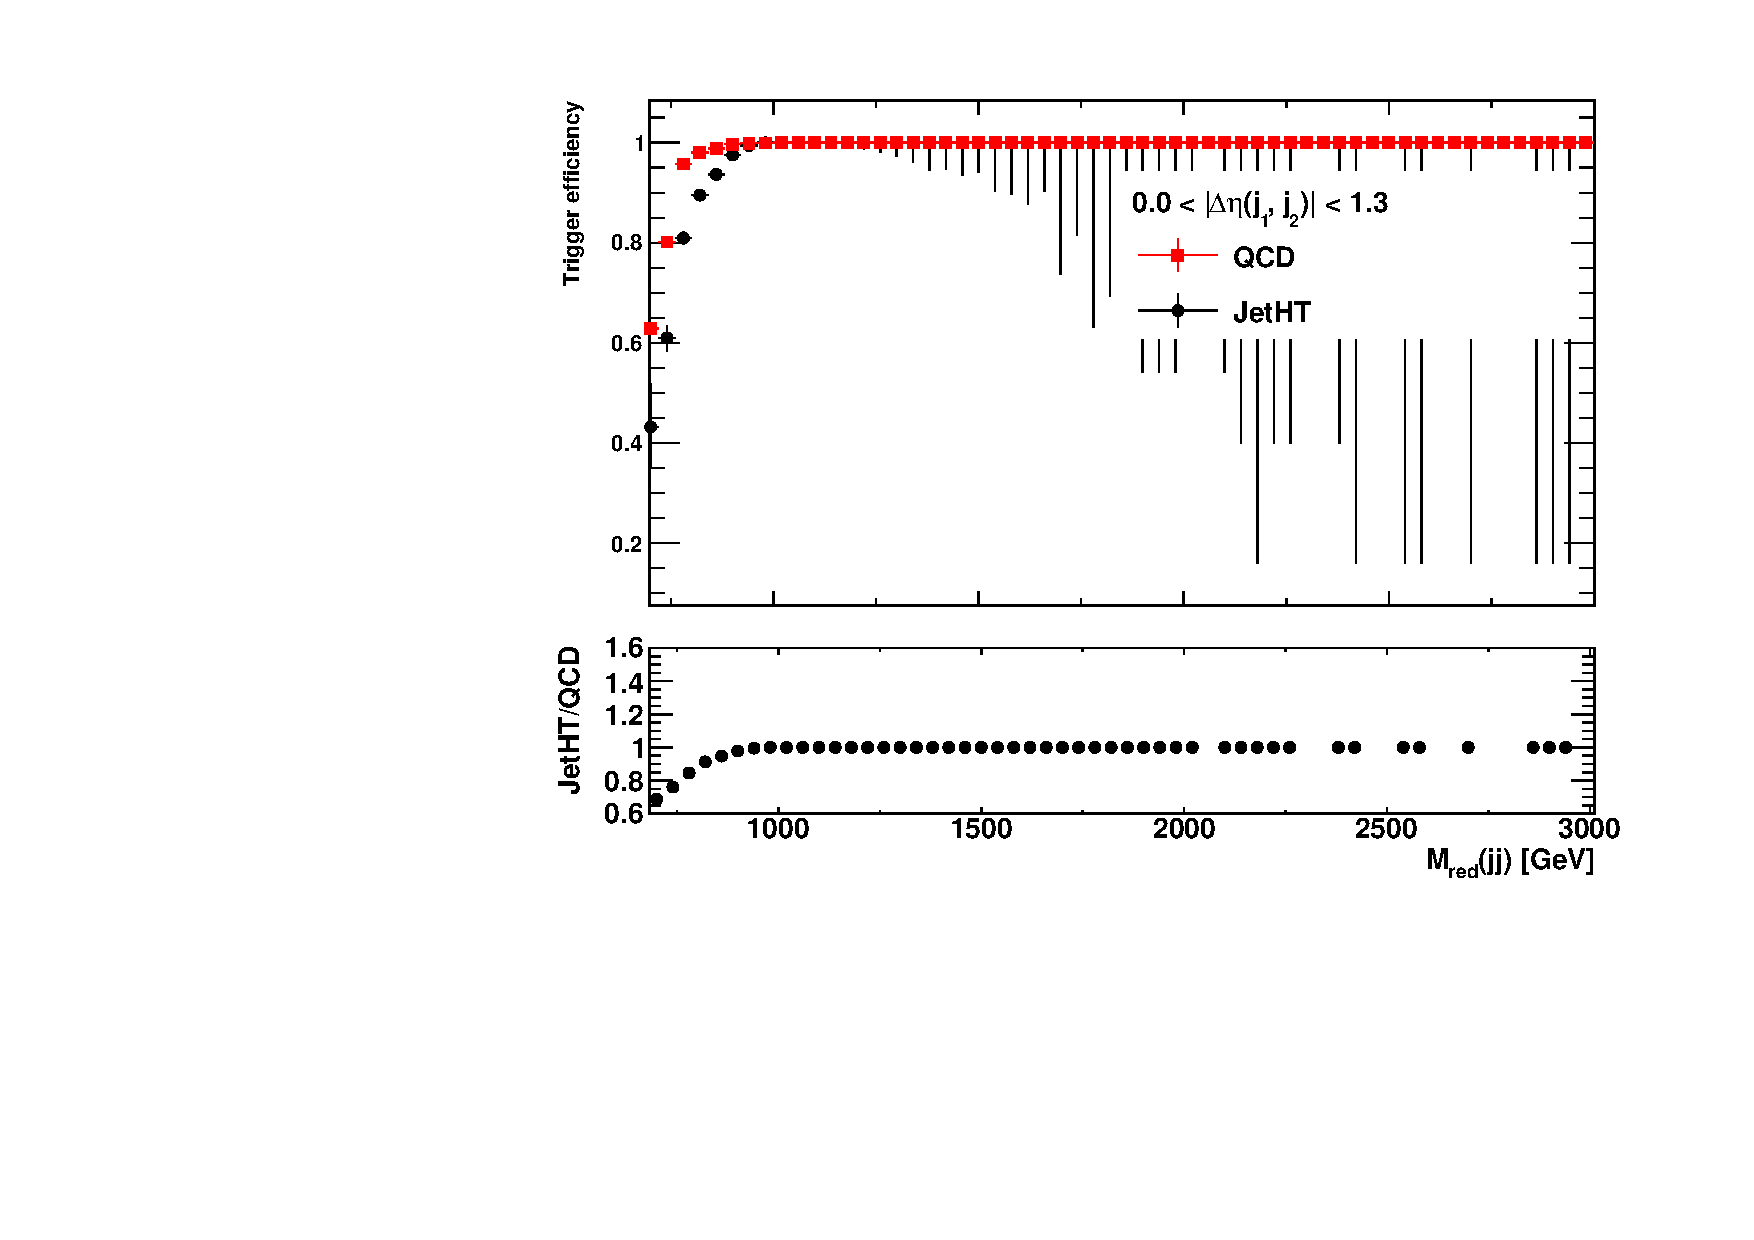
\includegraphics[width=0.45\textwidth]{Analysis/Trigger/JetHT_QCD_mjjred__trigEff.pdf}
    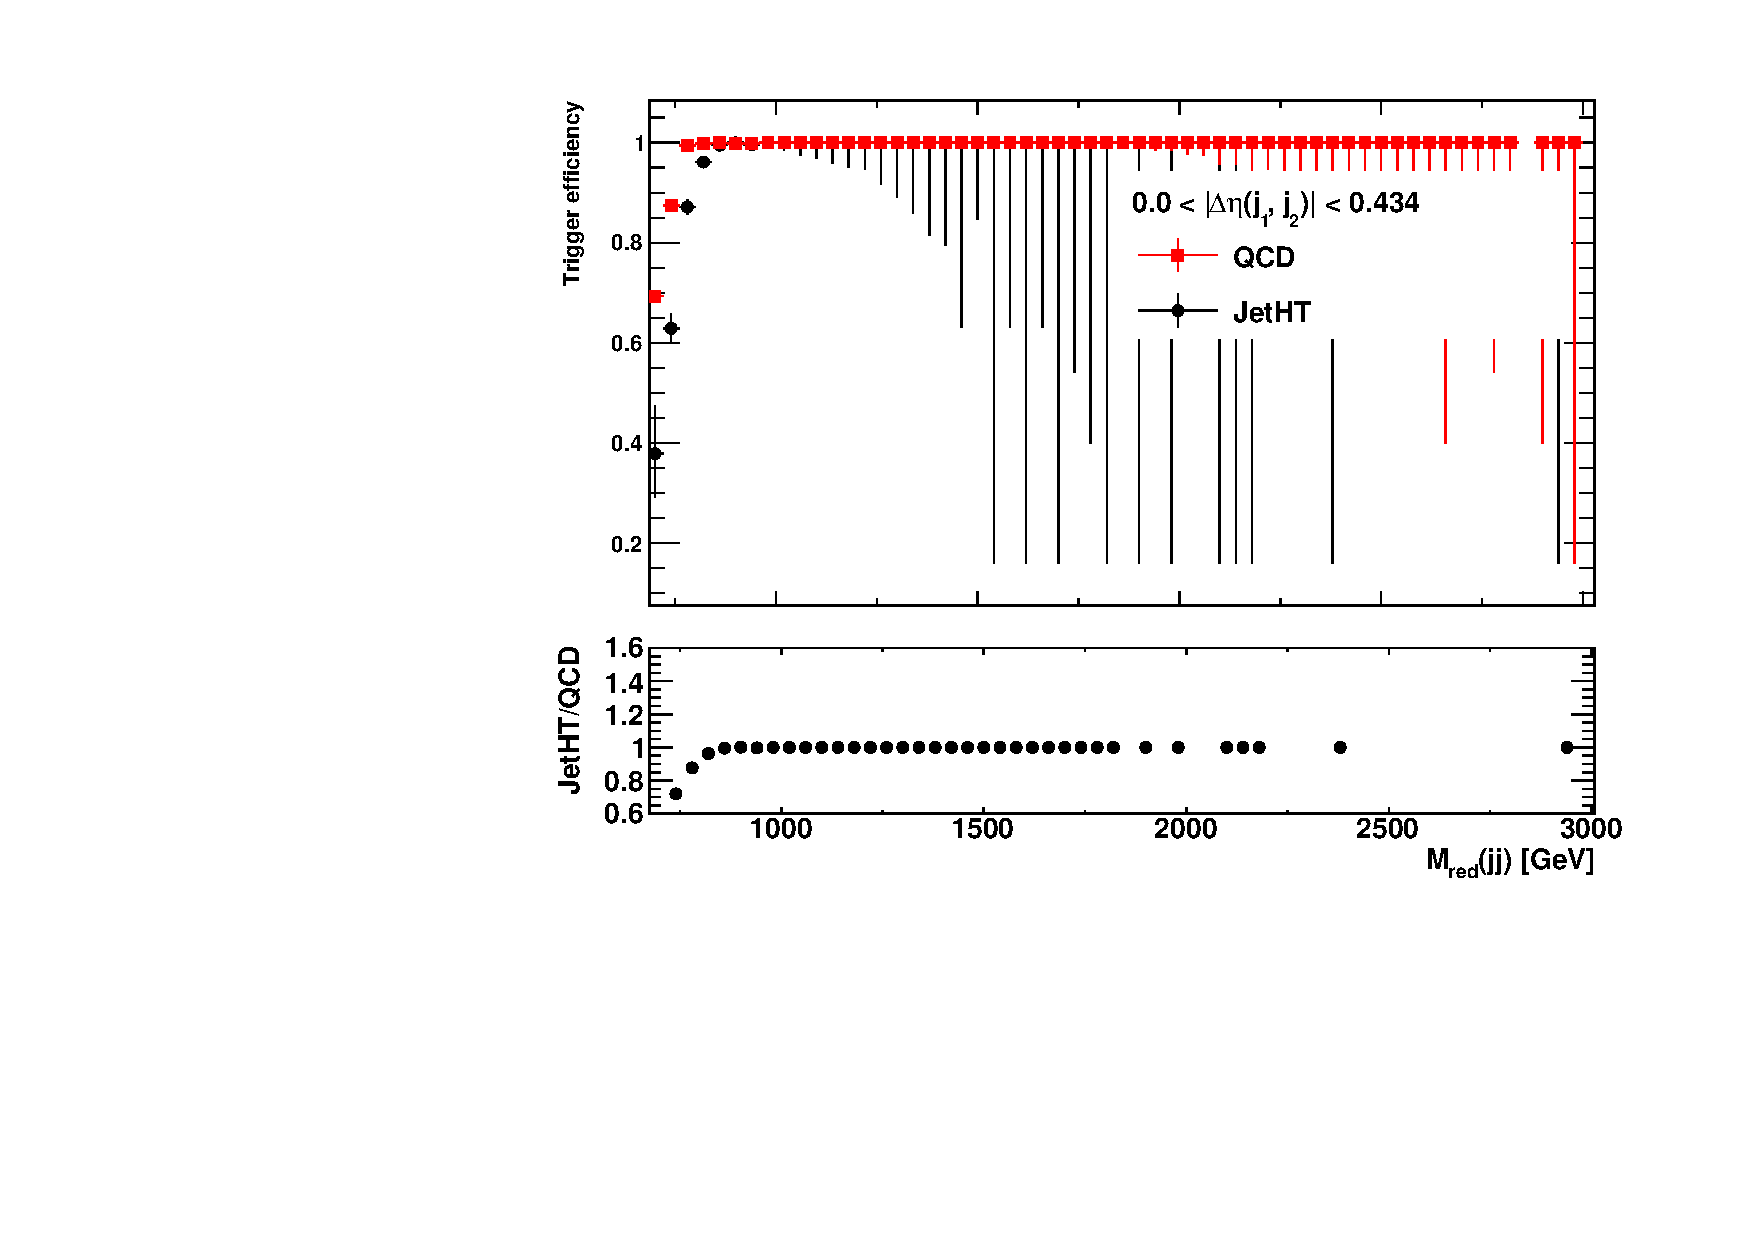
\includegraphics[width=0.45\textwidth]{Analysis/Trigger/JetHT_QCD_mjjred_py0_trigEff.pdf}

    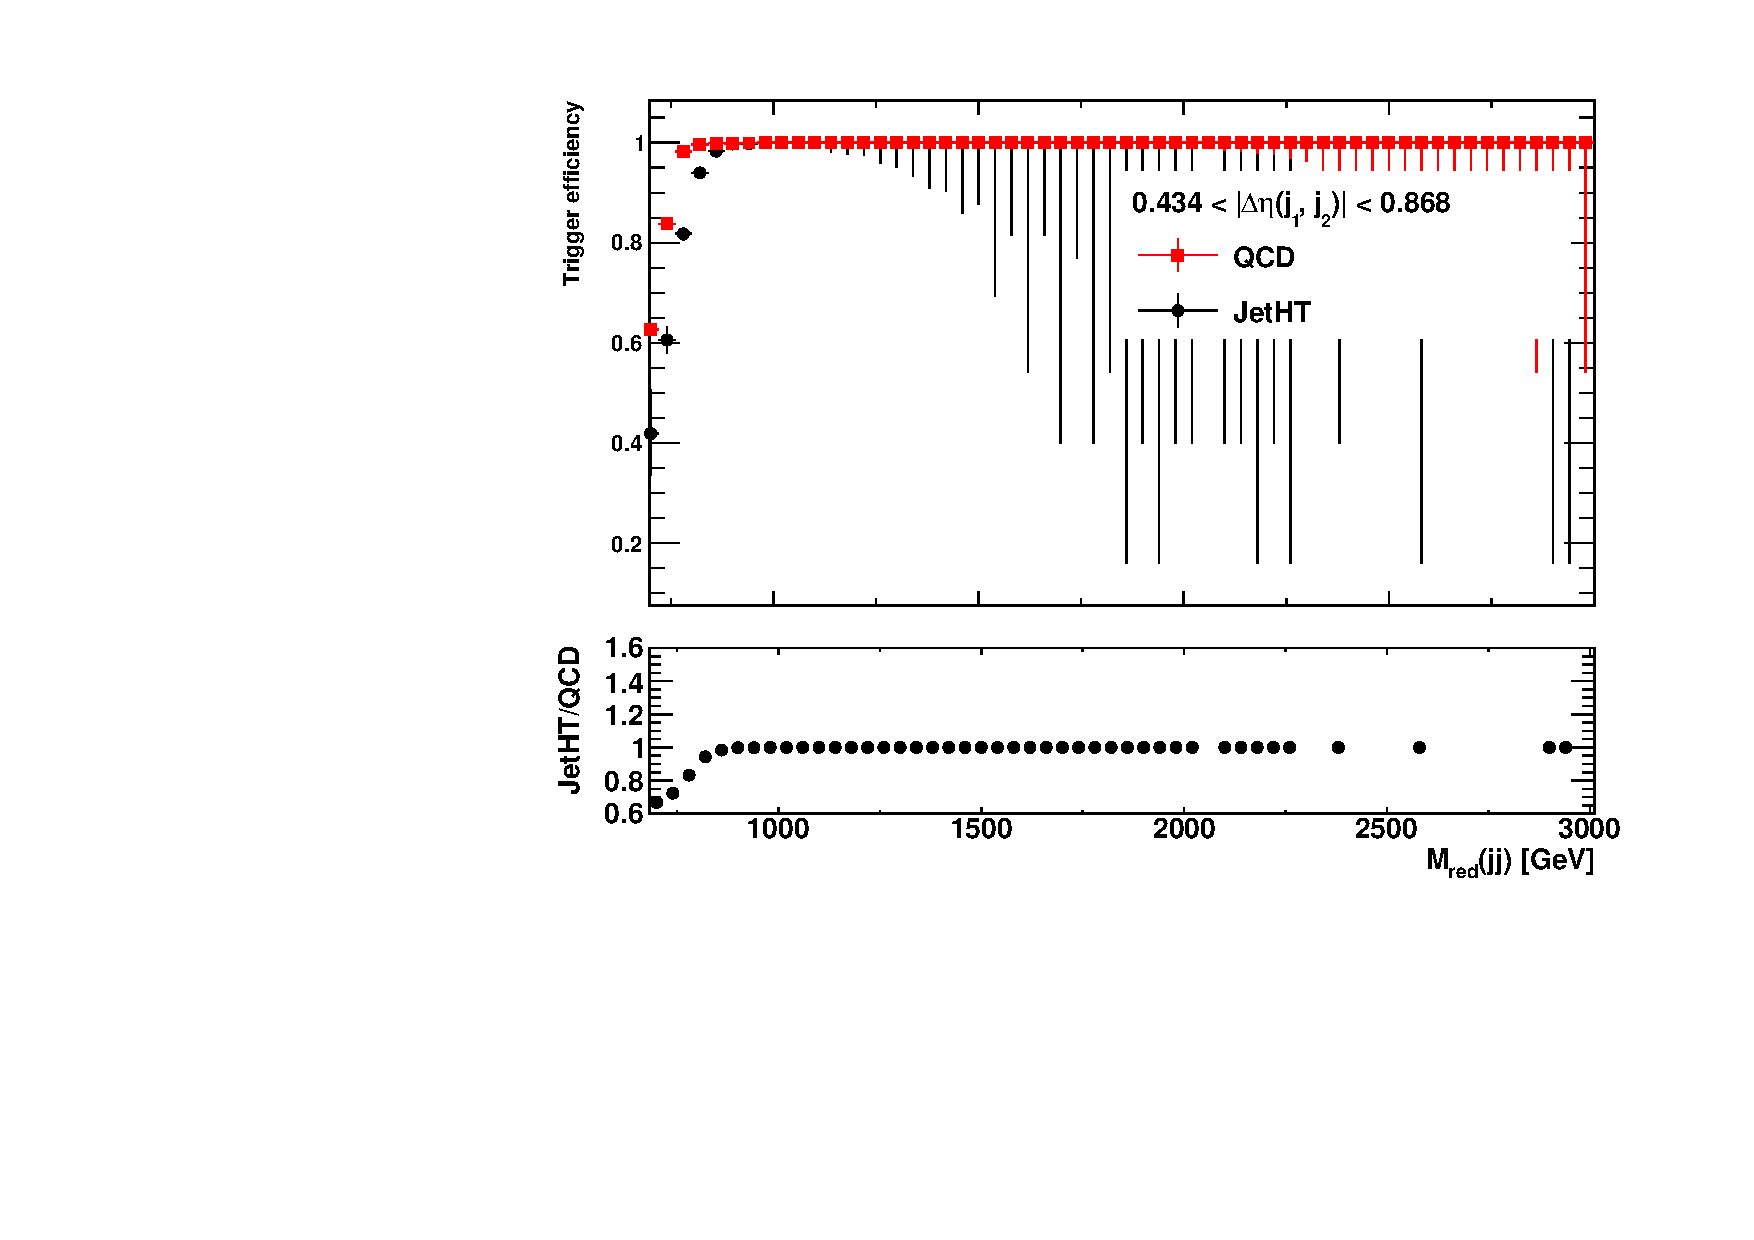
\includegraphics[width=0.45\textwidth]{Analysis/Trigger/JetHT_QCD_mjjred_py1_trigEff.pdf}
    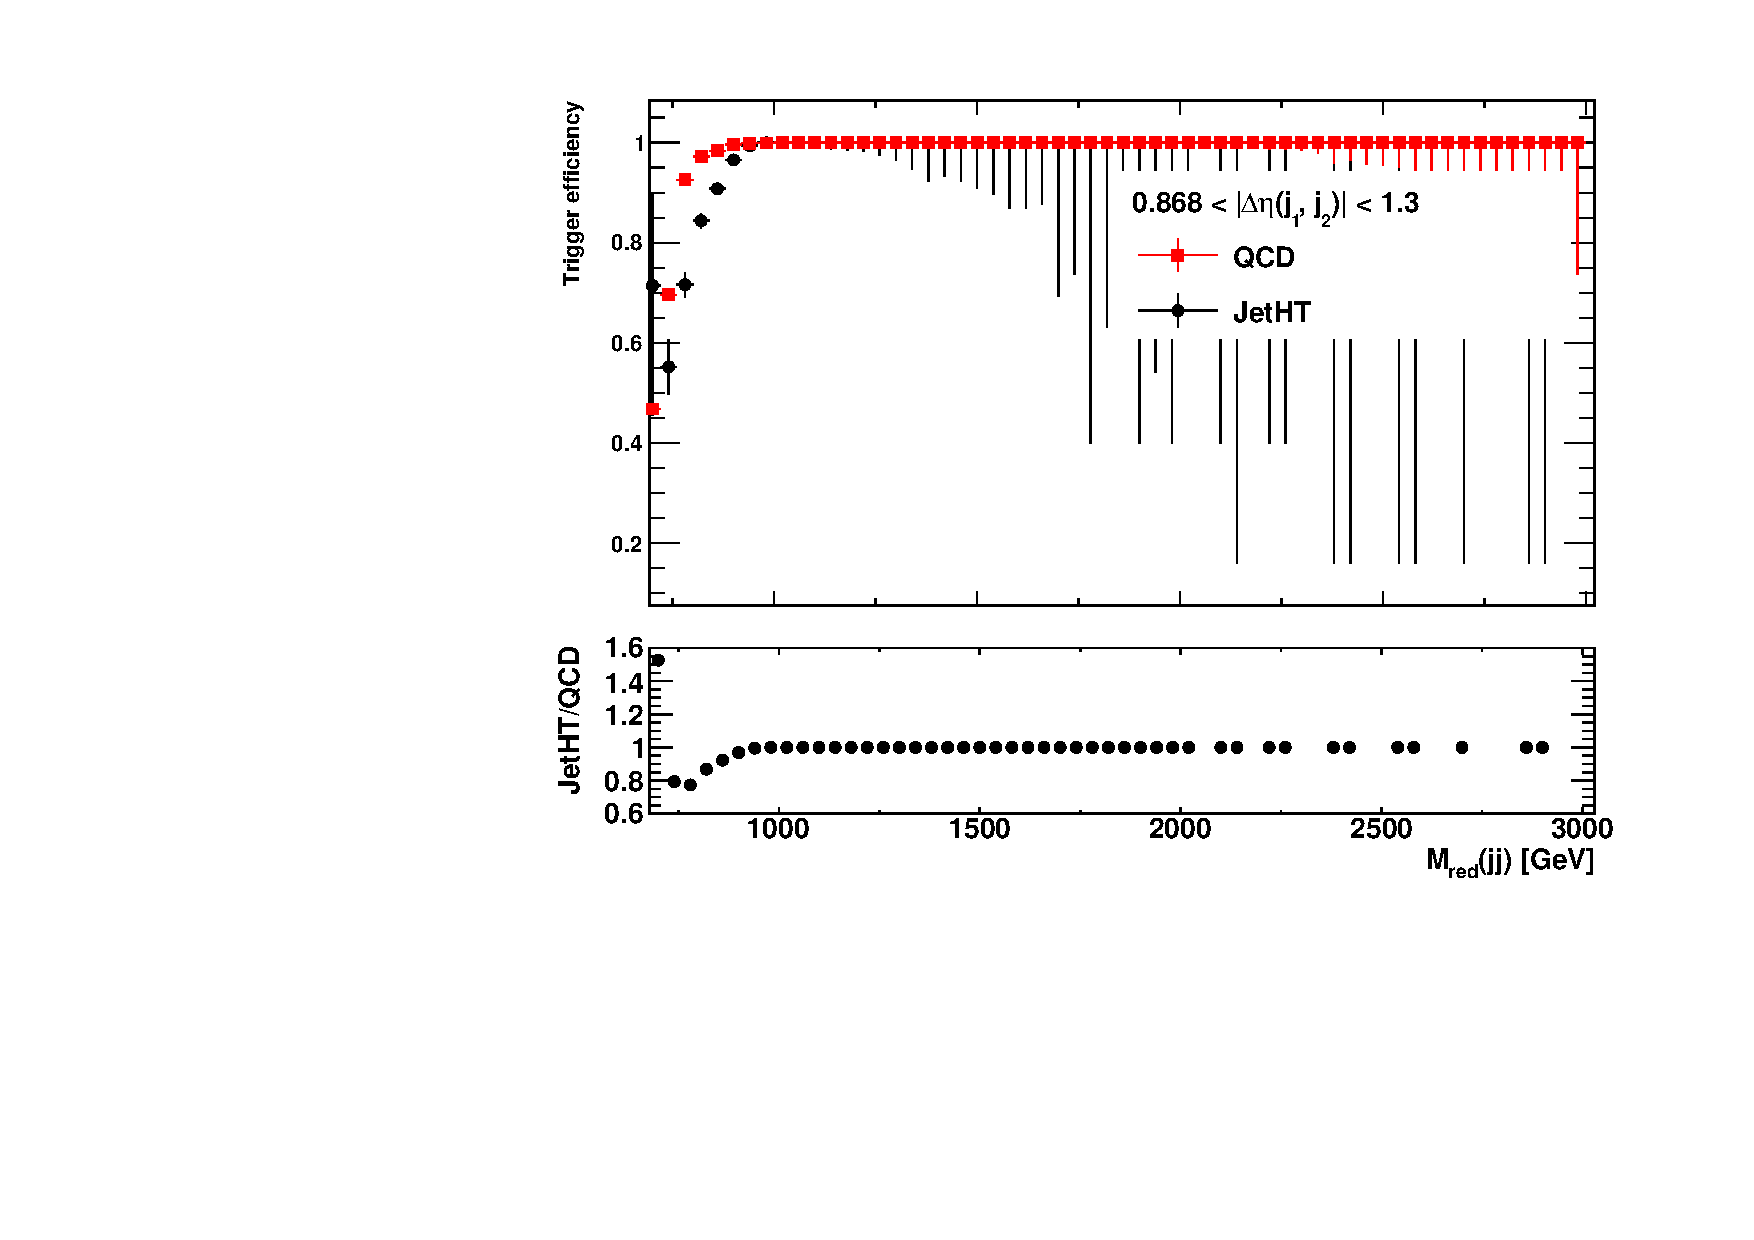
\includegraphics[width=0.45\textwidth]{Analysis/Trigger/JetHT_QCD_mjjred_py2_trigEff.pdf}
  \end{center}
  \caption{The trigger efficiency, as a function of $m_{jj}^{red}$, in the JetHT dataset and QCD MC for different $|\Delta\eta(\mathrm{j}_{1}, \mathrm{j}_{2})|$ regions: $0.0-1.3$ (upper left), $0.0-0.434$ (upper right), $0.434-0.868$ (lower left), and $0.868-1.3$ (lower right).}
  \label{fig:trigeEffvsMjj_JetHT_DetaBins}
\end{figure}

\begin{figure}[h!]
  \begin{center}
    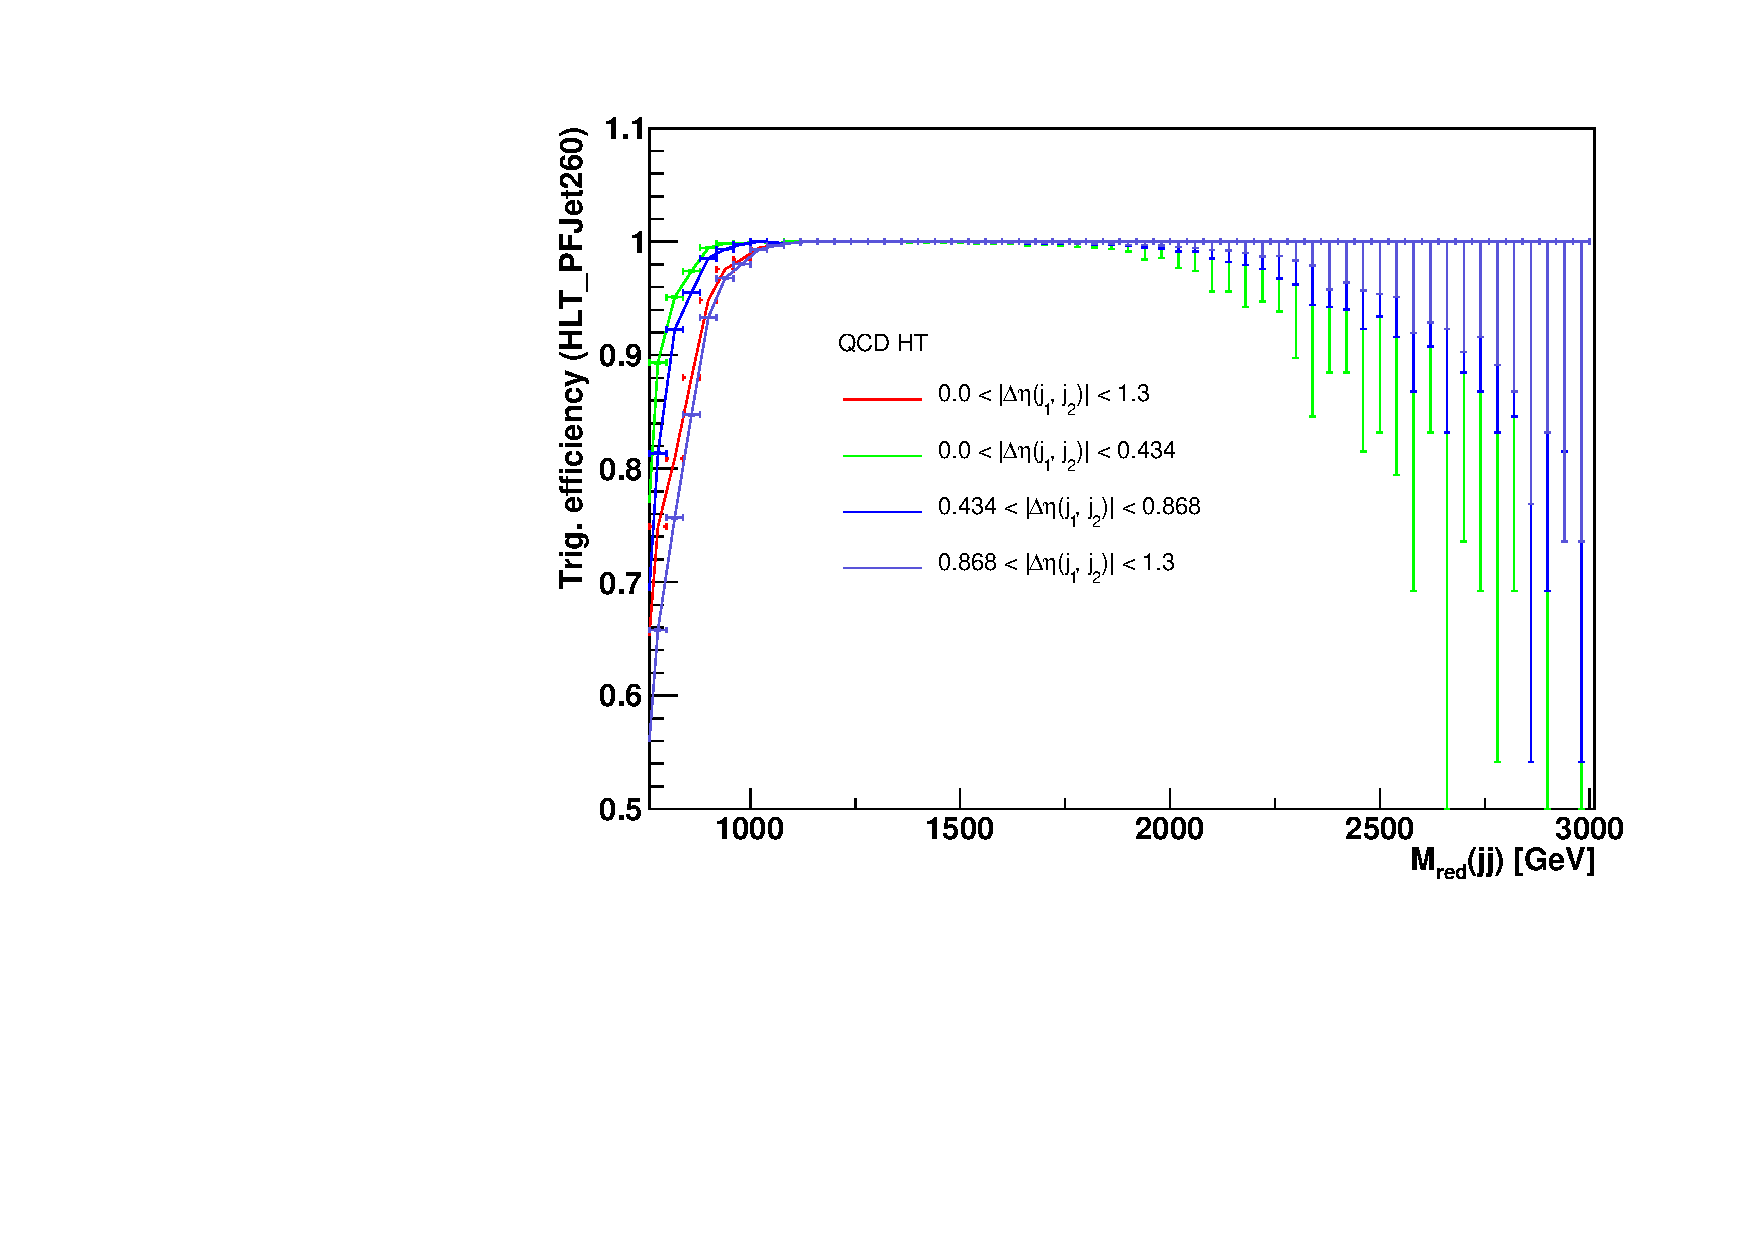
\includegraphics[width=4 in]{Analysis/Trigger/c_QCD_HLTPFJet260.pdf}
  \end{center}
  \caption{The trigger efficiency in QCD MC for the baseline trigger \textsc{HLT\_PFJet260}, as a function of $m_{jj}^{red}$, for different $|\Delta\eta(\mathrm{j}_{1}, \mathrm{j}_{2})|$ regions: $0.0-1.3$, $0.0-0.434$, $0.434-0.868$, and $0.868-1.3$. The percentage difference between one and these turn-on curves is taken as an uncertainty on the trigger efficiency scale factor.}
  \label{fig:trigeEffvsMjj_QCDHT_HLTPFJet260_DEtabins}
\end{figure}

Since the search begins from $m_{jj}^{red} = 750$ GeV, the modeling of the trigger efficiency curves in data and simulation is done extremely carefully. Originally, the trigger efficiency was measured using an orthogonal trigger path \texttt{HLT\_Mu50}. However, the switch to the \texttt{HLT\_PFJet260} trigger was made because the final event selection vetoes events with isolated leptons and therefore the \texttt{HLT\_Mu50} selection is completely orthogonal to the signal region. The baseline trigger \texttt{HLT\_PFJet260} has some inefficiency for low $m_{jj}^{red}$ and therefore an additional uncertainty is assigned to the trigger efficiency scale factor based on this trigger's efficiency  in MC. Figure~\ref{fig:trigeEffvsMjj_QCDHT_HLTPFJet260_DEtabins} shows the \texttt{HLT\_PFJet260} trigger turn-on curves for different $|\Delta\eta(\mathrm{j}_{1}, \mathrm{j}_{2})|$ in MC, with respect to only the event selection. The difference between unity and the trigger efficiency is propagated to the scale factor as a systematic uncertainty. 

%\begin{figure}[h]
%  \begin{center}
%    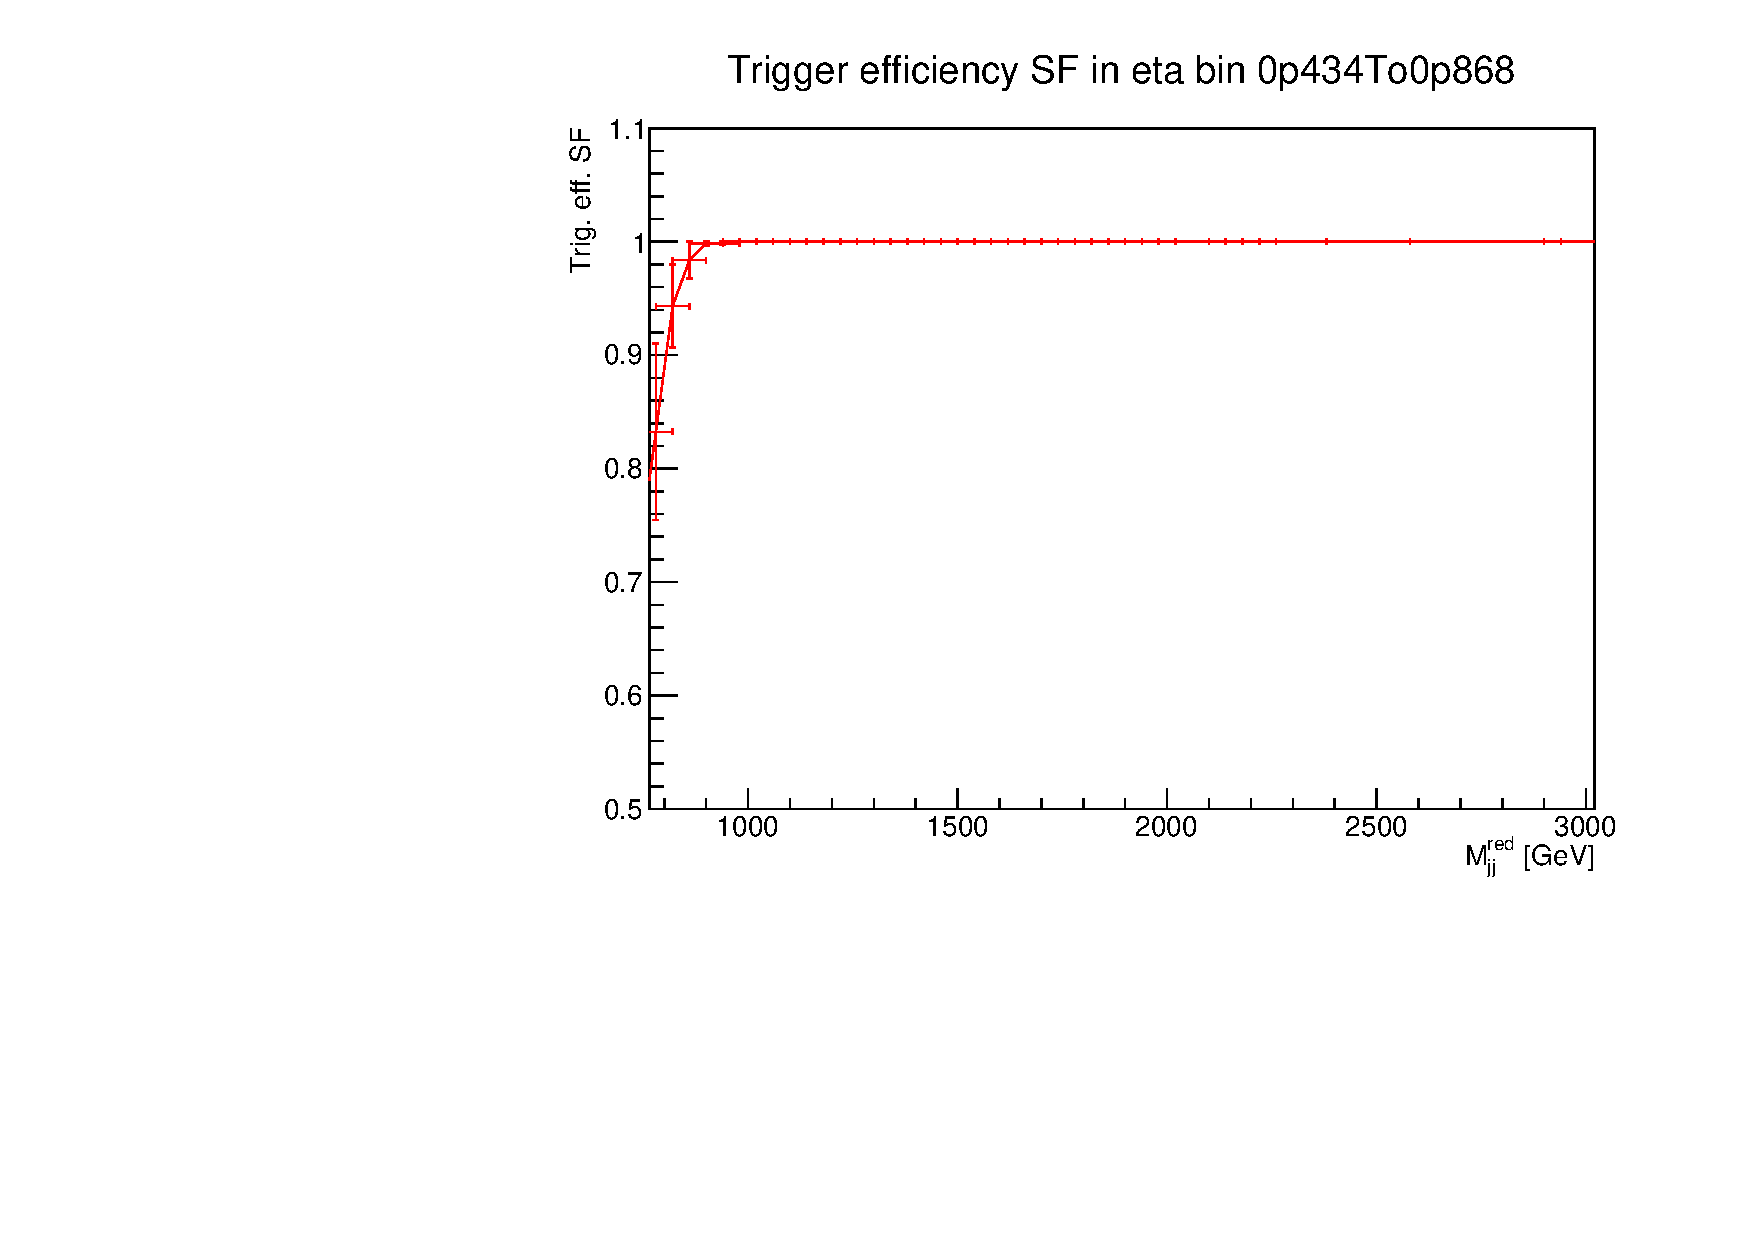
\includegraphics[width=0.33\textwidth]{Analysis/Trigger/c_gsftrigger_0p434To0p868}
%    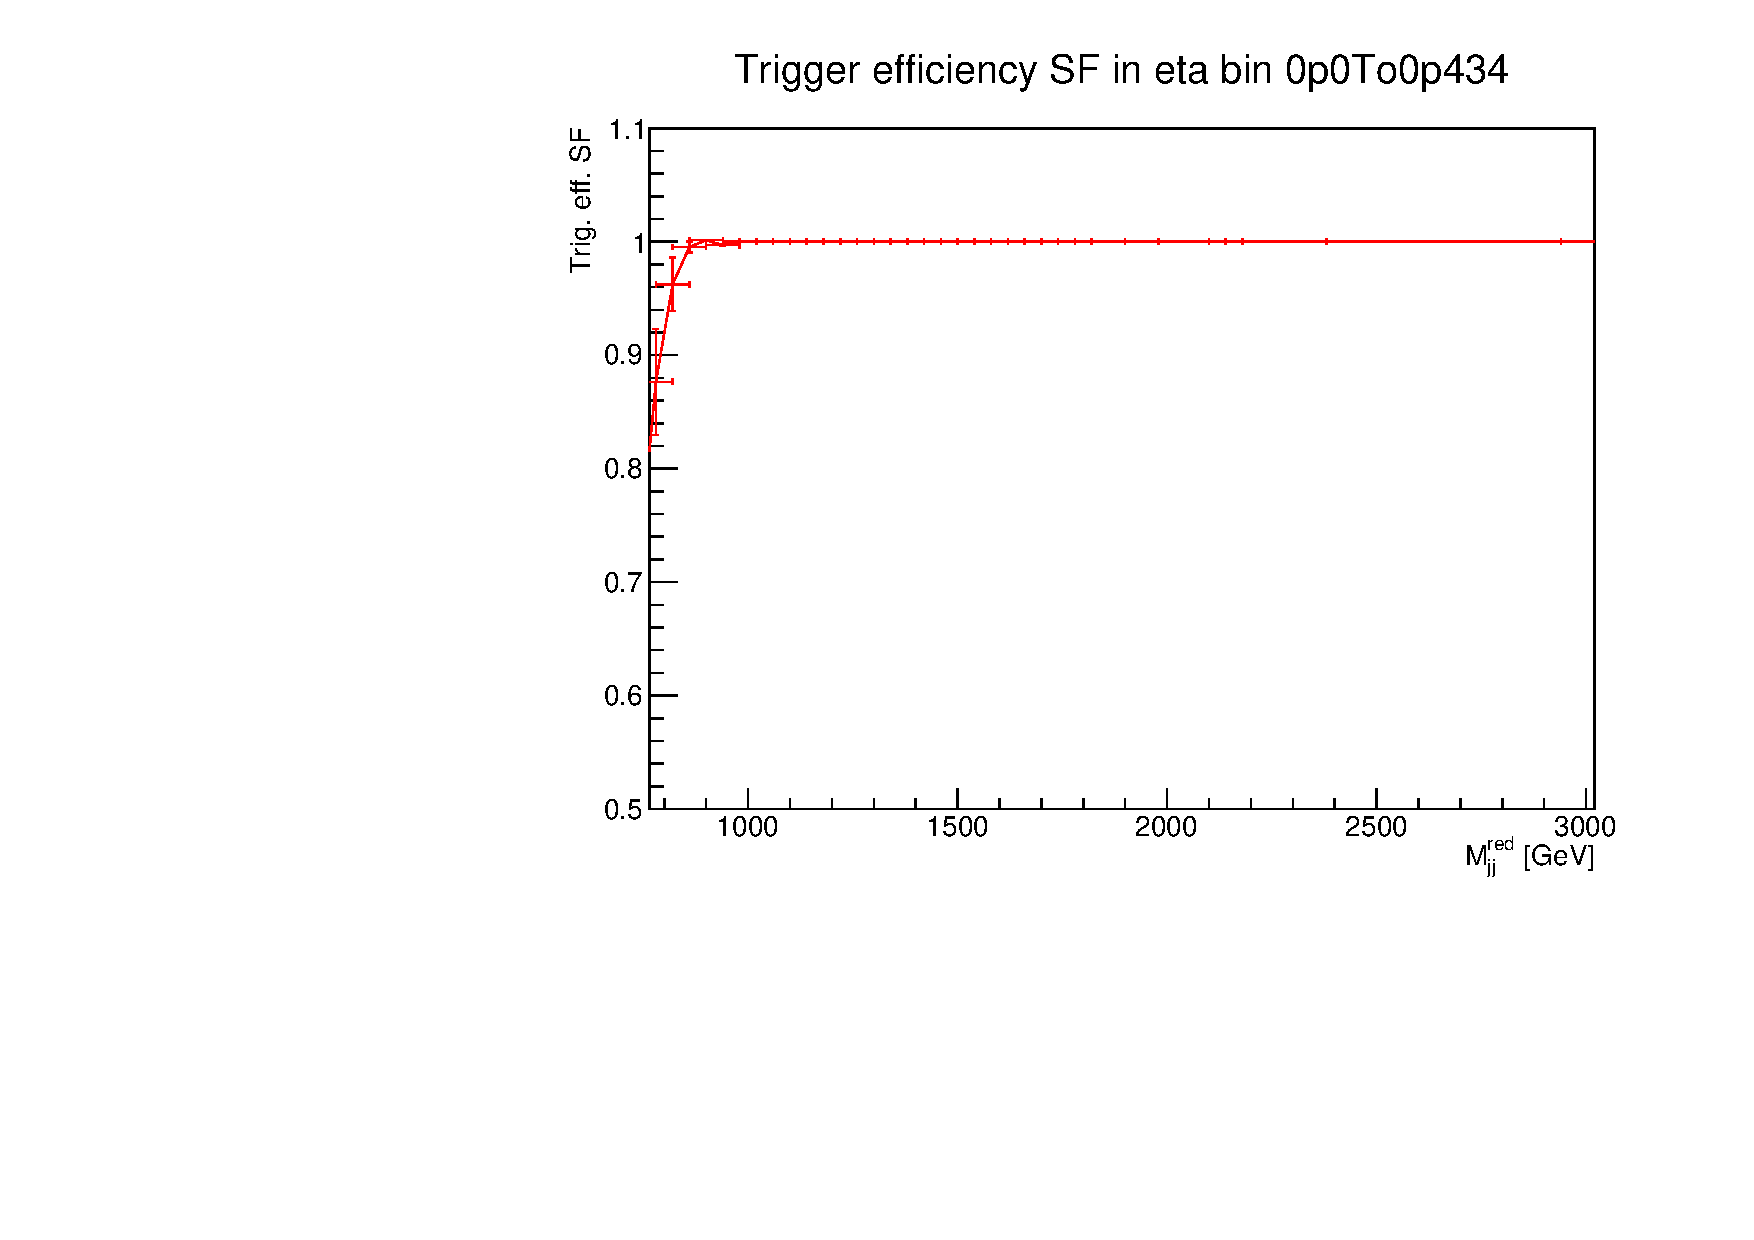
\includegraphics[width=0.33\textwidth]{Analysis/Trigger/c_gsftrigger_0p0To0p434}
%    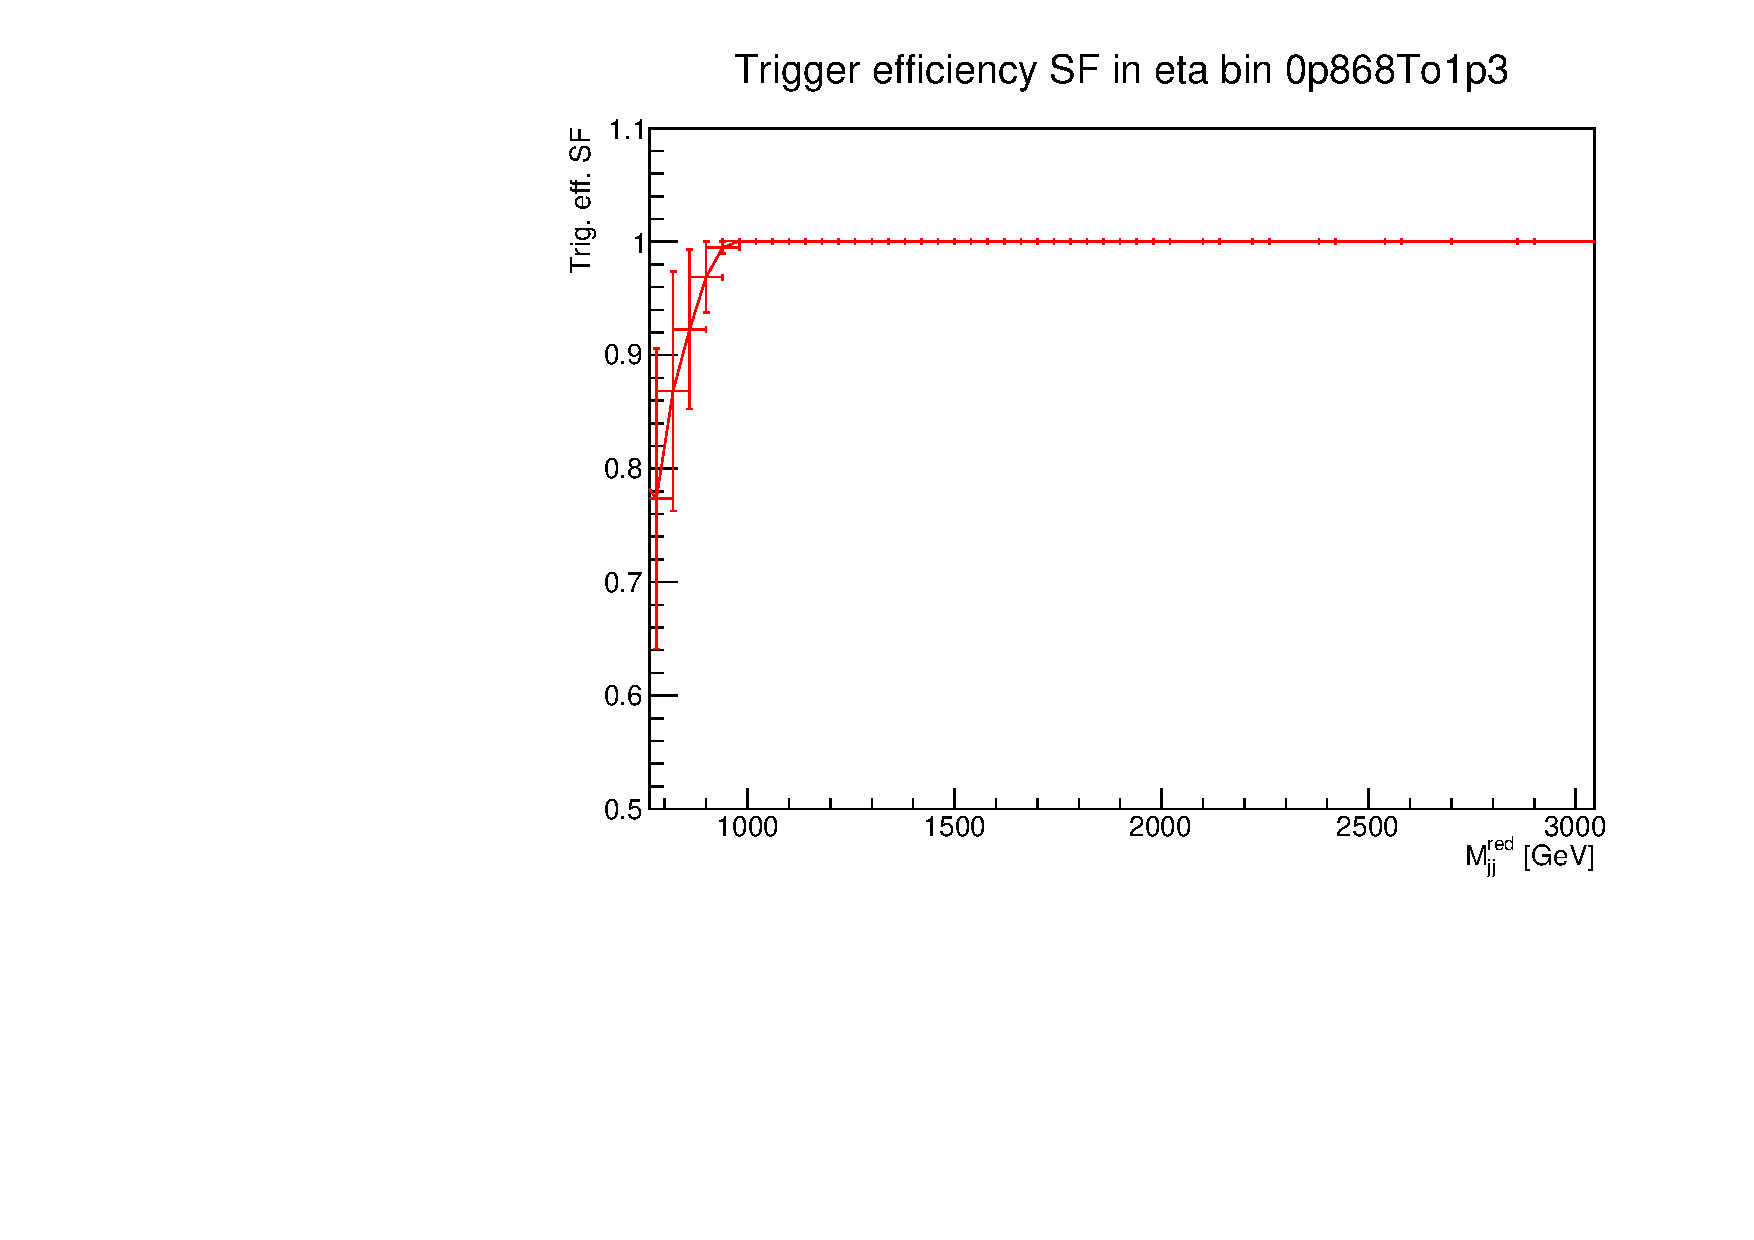
\includegraphics[width=0.33\textwidth]{Analysis/Trigger/c_gsftrigger_0p868To1p3}
%  \end{center}
%  \caption{The trigger efficiency scale factors, as a function of $M_{jj}^{red} \equiv M_{jj} - (M_{jet}^{1}-M_{H}) - (M_{jet}^{2}-M_{H})$, defined in %Section~\ref{}, for different $\Delta\eta_{jj}$ regions: 0.0--0.434 (left), 0.434--0.868 (centre), and 0.868--1.3 (right). The error bars are the combined %statistical and systematic errors.}
%  \label{fig:trigeEffSFvsMjj_JetHT_DetaBins}
%\end{figure}


%\begin{figure}[h]
%  \begin{center}
%    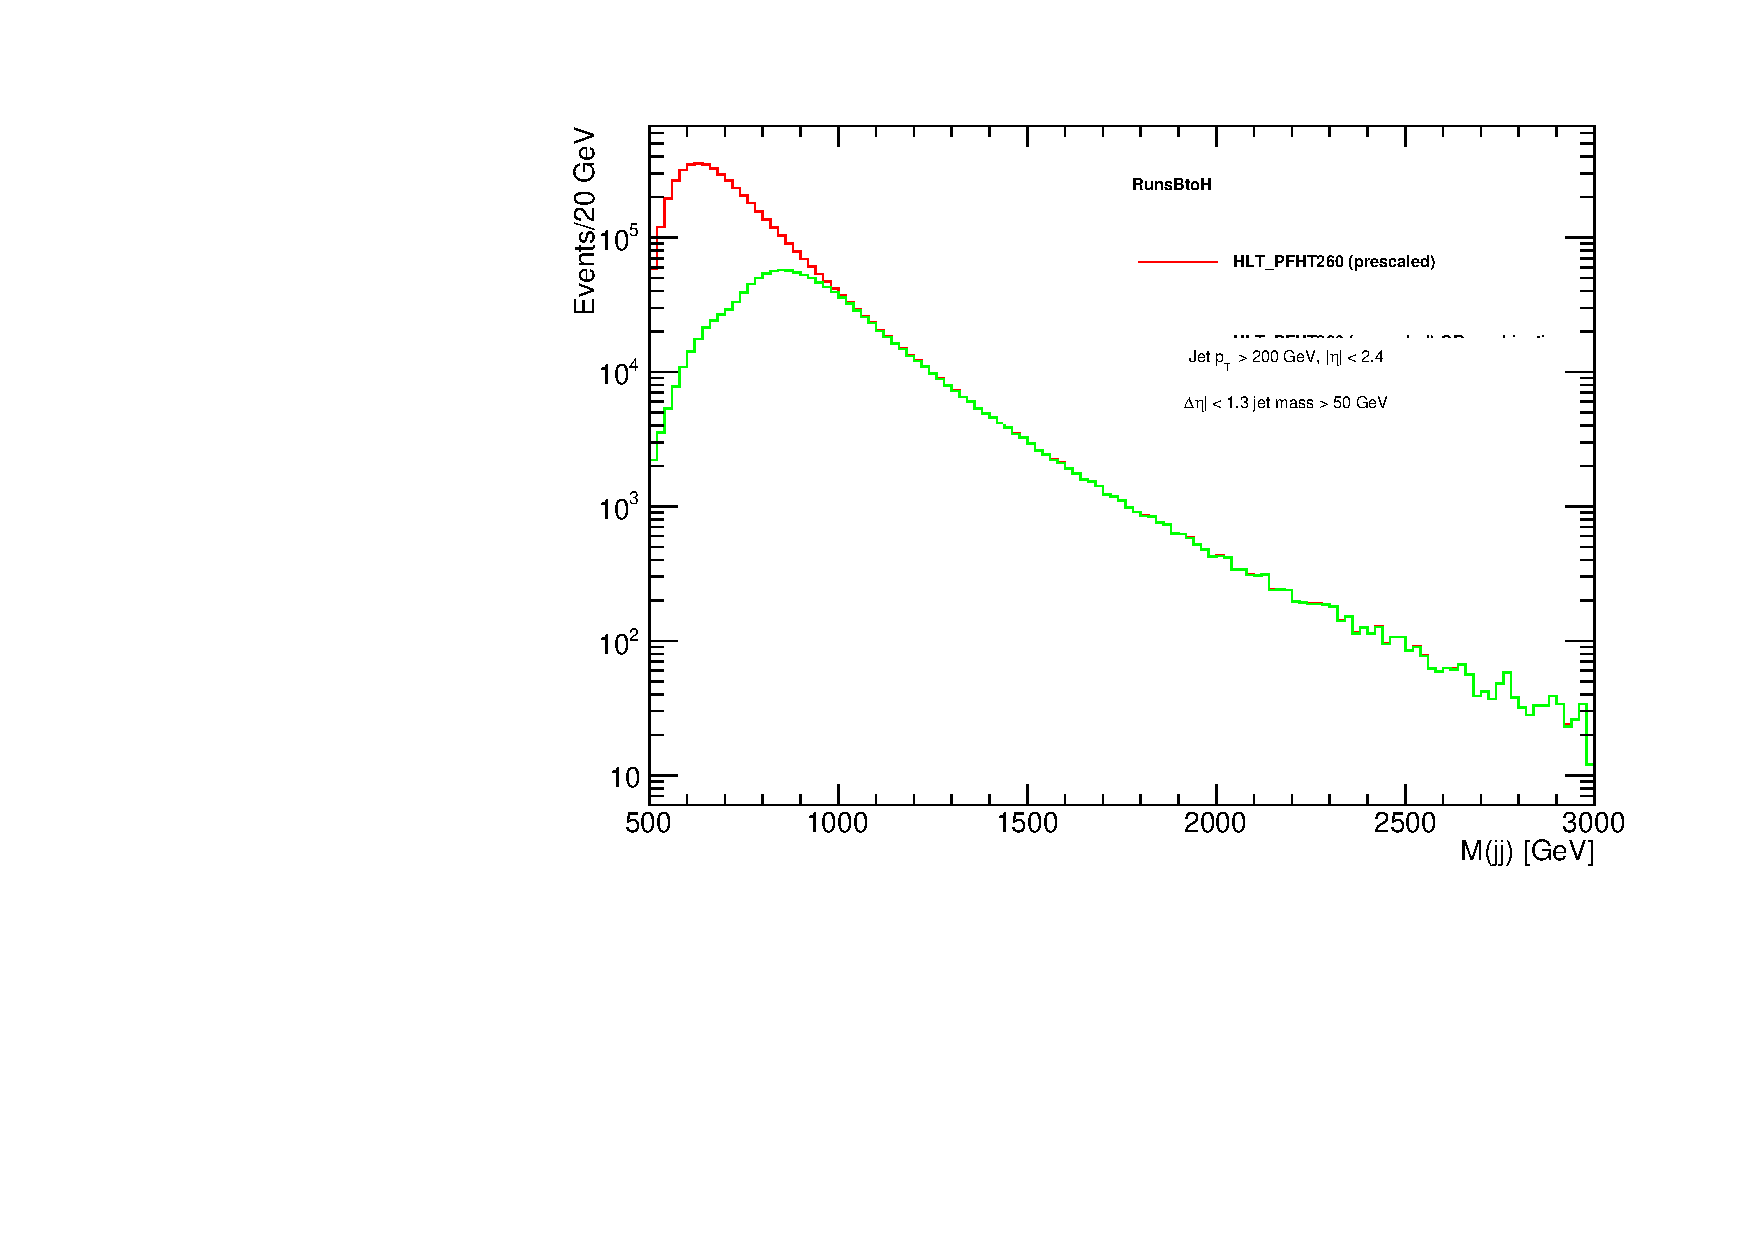
\includegraphics[scale=0.32]{Analysis/Trigger/JetHT_RunsBtoH_mjj_all_pass.pdf}
%    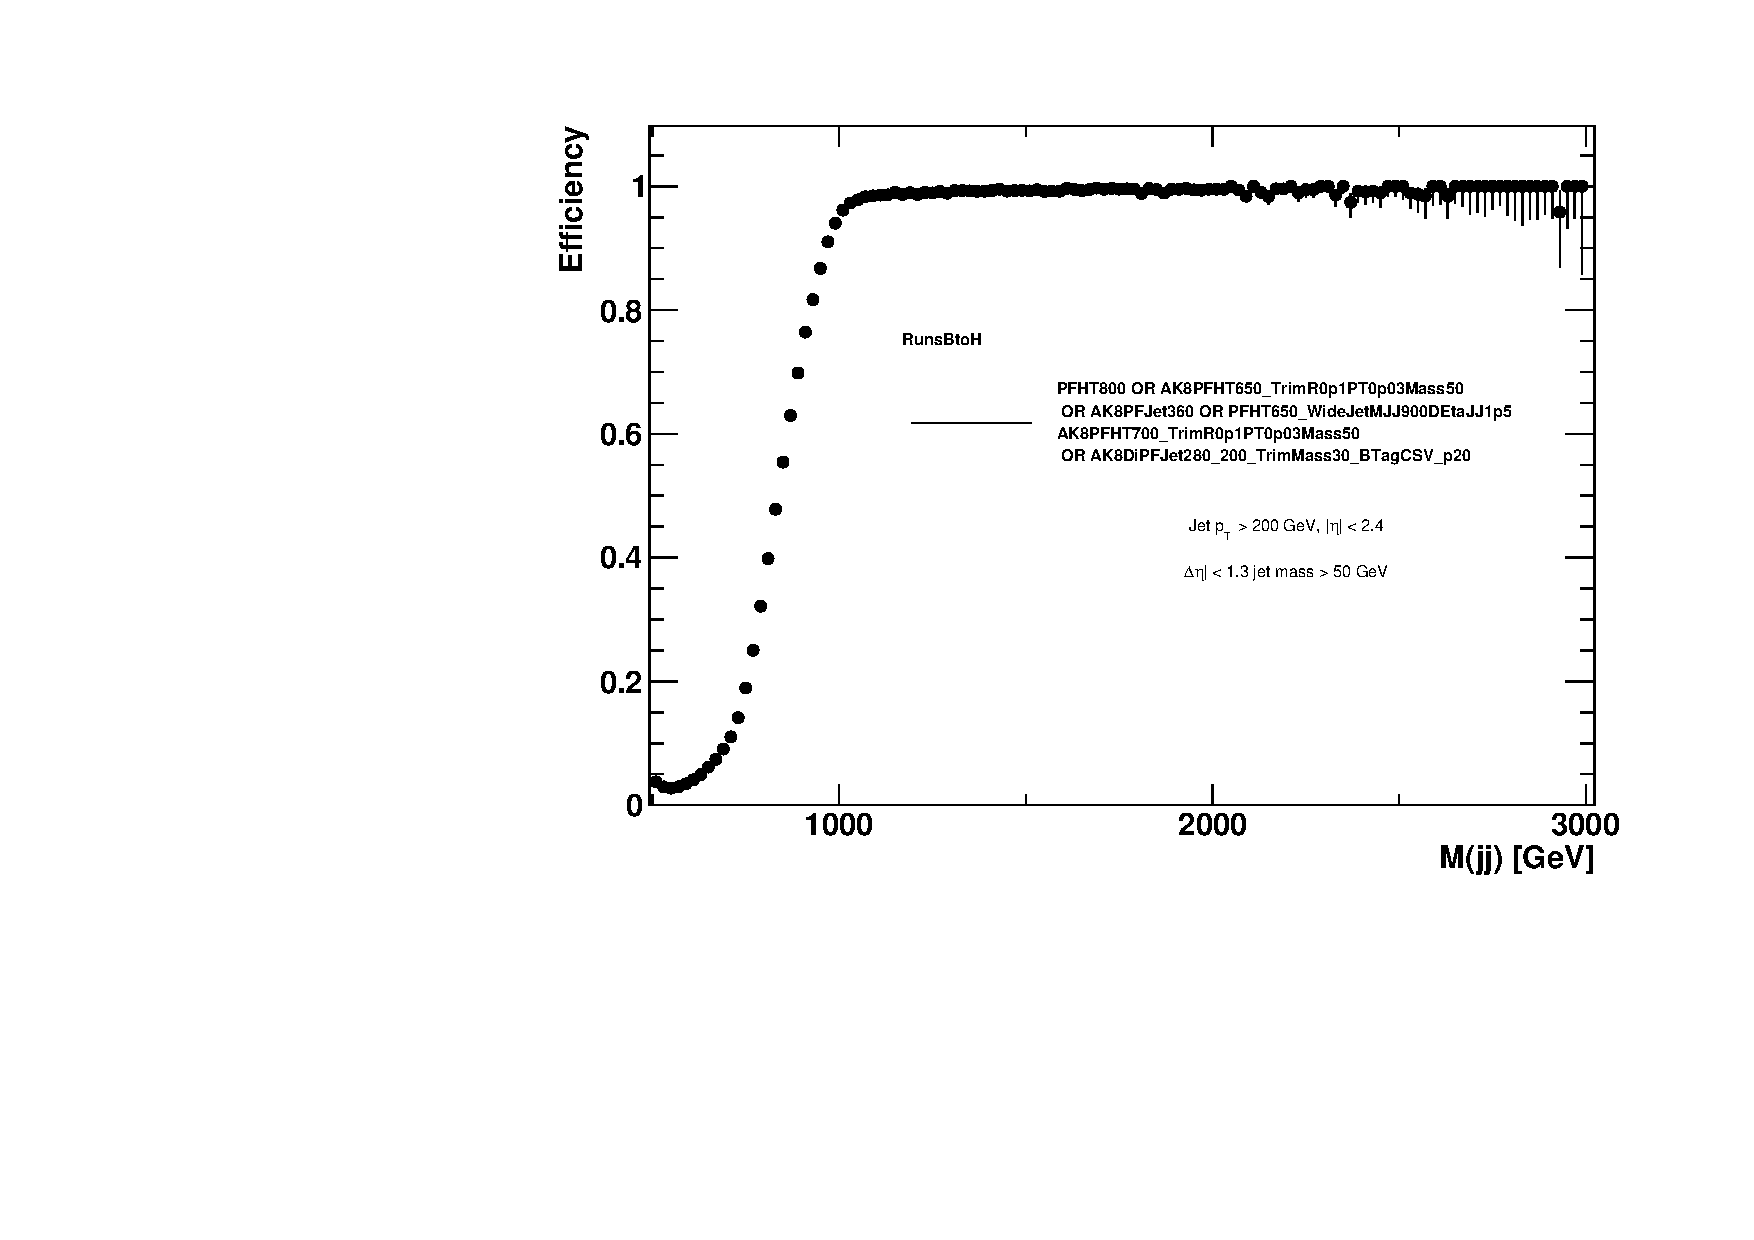
\includegraphics[scale=0.32]{Analysis/Trigger/JetHT_RunsBtoH_trigeff_mjj.pdf}
%    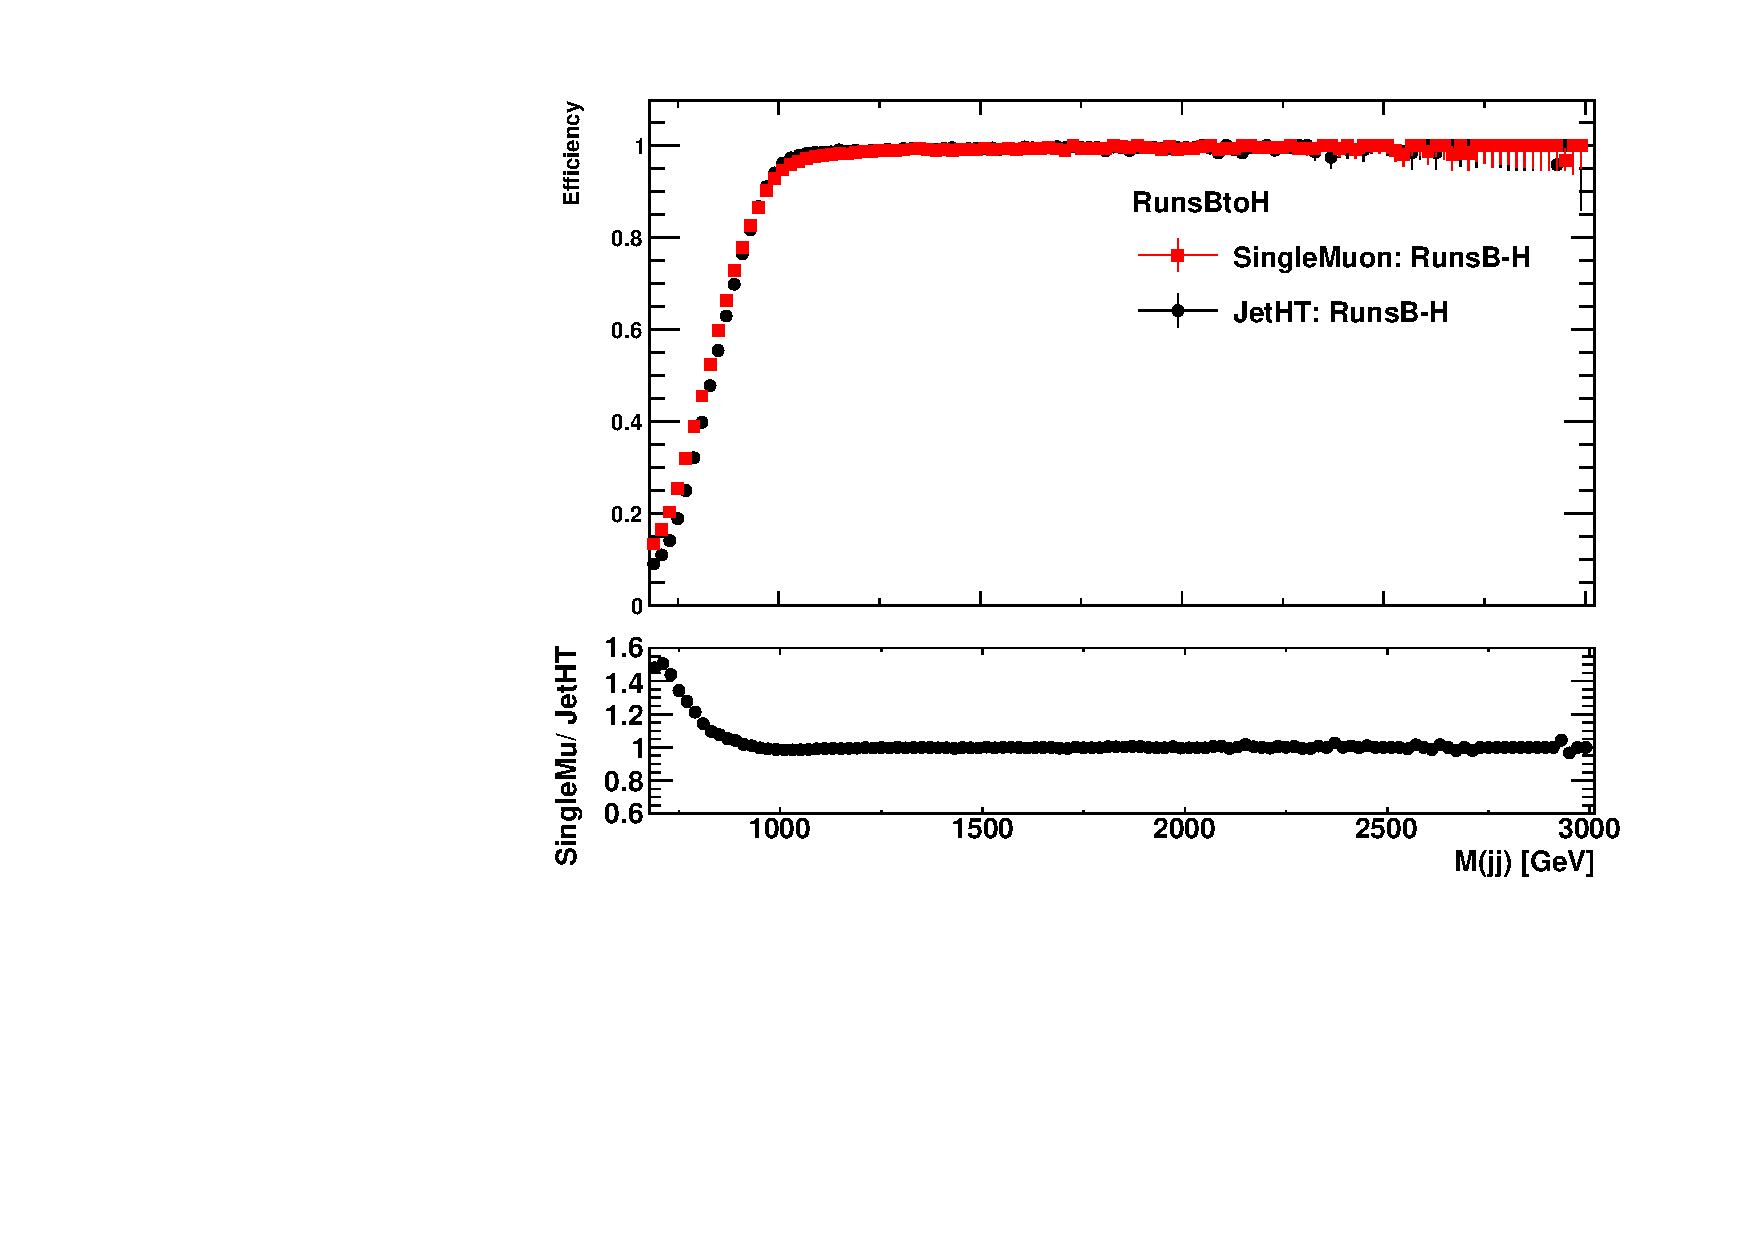
\includegraphics[scale=0.32]{Analysis/Trigger/JetHT_SingleMuon_BtoH_mjj_trigEff.pdf}
%  \end{center}
%  \caption{The dijet mass distribution used to derive the efficiency in data (top left) and the trigger efficiency as measured in data (top right) using the \texttt{JetHT} dataset. The bottom figure shows the ratio of the turn-on curves from the \texttt{SingleMuon} over the \texttt{JetHT} datasets.}
%  \label{fig:Mjj_trigeEffvsMjj_JetHT}
%\end{figure}

\section{Event Selection}
\label{sec:EvtSel}

%The search for HH resonant production in the four b quark decay channel is an all hadronic final state which means that a big challenge for this analysis is reducing the large amount of QCD background events in the signal region. 

After passing the triggers, events are required to have at least one reconstructed $pp$ collision vertex satisfying the following criteria:
\begin{itemize}
  \item Vertex number of degrees of freedom $> 4$.
  \item Absolute displacement from the beamspot position along the $z$ direction $< 24$ cm.
  \item Absolute displacement from the beamspot position along the transverse direction $< 2$ cm.
\end{itemize}

\noindent
Many additional vertices, corresponding to other overlapping $pp$ collisions (pileup), are usually reconstructed in an event using charged particle tracks. The primary interaction vertex (PV) corresponds to the vertex that maximizes the sum in $p_{T}^2$ and the magnitude of $\sum{p_{T}}$ from the associated physics objects.

\subsection{Lepton Selection}

To suppress $\mathrm{t\bar{t}}$ and diboson backgrounds, events containing an isolated electron or muon with $p_{T} > 20$ GeV are removed. The isolation requirement is designed to remove jets misidentified as leptons and is defined as the ratio of energy surrounding the lepton and the lepton's momentum. The energy surrounding a lepton is the scalar $p_{T}$ sum of the charged hadrons, neutral hadrons, and photons in a cone with size $\Delta R = 0.3$ and $\Delta R = 0.4$ for electrons and muons, respectively. The identification criteria for an electron is listed in Table~\ref{tab:electronid} and the muon identification criteria is listed in Table~\ref{tab:muonid}. The combined isolation and identification requirement of the electron is such that the overall selection efficiency is $90\%$ ($70\%$) for the ``loose" (``medium") requirement. For the ``loose" (``medium") muons, the selection efficiency is $100\%$ ($95\%$). Events are rejected if they contain one lepton passing the medium requirement or two leptons passing the loose requirement that have the same flavor but opposite charge.

\begin{table}[htb]
  \begin{center}
    \begin{tabular}{l |l | l | l | l}
    \hline
    \hline
       & \multicolumn{2}{c}{Barrel Selection} &
    \multicolumn{2}{| c}{Endcap Selection}\\
    \hline
    Variable & Loose &  Medium & Loose & Medium\\
    \hline
    $5\times 5\: \sigma_{i\eta i\eta} < $ & 0.011 & 0.00998 & 0.0314 & 0.0298  \\
    $\Delta \eta_{seed} < $ & 0.00477 & 0.00311 & 0.00868 & 0.00609  \\
    $\Delta \phi_{in} <$  & 0.222 & 0.103 & 0.213 & 0.045     \\
    H/E $<$   & 0.298 & 0.253 & 0.101 & 0.0878   \\
    $|\frac{1}{E} - \frac{1}{p}| <$ & 0.241 & 0.134 & 0.14 & 0.13   \\
    Missing hits $\leq$   & 1 & 1 & 1 & 1     \\
    Conversion veto     & yes & yes & yes & yes \\
    \hline
    \hline
    \end{tabular}
   \caption{Loose and medium electron identification criteria used in the analysis. The selection criteria varies depending on if the electron is in the barrel or endcap of the detector. $\sigma_{i\eta i\eta}$ is the energy weighted standard deviation of a single crystal within the $5\times 5$ cluster of crystals centered at the crystal with maximum energy and H/E refers to the energy measured in the hadronic calorimeter divided by the energy measured in the electromagnetic calorimeter.\label{tab:electronid}}
  \end{center}
\end{table}

\begin{table}[h!]
  \begin{center}
    \begin{tabular}{l | l}
    \hline
    \hline
    Loose &  Medium \\
    \hline
    Global or Tracker Muon     & Global Muon  \\
    PF Muon  & Normalized $\chi^{2}$ of the global track $< 3$     \\
      & Tracker-Standalone position match $< 12$  \\
      & Kink finder $< 20$     \\
      & segment compatibility $> 0.303$      \\
      & OR \\
      & segment compatibility $> 0.451$ \\
    \hline
    \hline
    \end{tabular}
   \caption{Loose and medium muon identification criteria used in the analysis.\label{tab:muonid}} %A segment is when hits in the muon drift tubes and cathode strip chambers are matched.\label{tab:muonid}}
  \end{center}
\end{table}

\subsection{Jet Selection}

Particle Flow (PF) candidates are clustered using the anti-$k_{t}$ algorithm~\cite{antikt}, implemented in \textsc{FastJet}~\cite{FastJet}, into jets with a distance parameter $R=0.8$ (referred to as AK8 jets). To mitigate the effect of pileup, particles are assigned weights using the pileup per particle identification (PUPPI) algorithm~\cite{PUPPI}. This method uses local shape information, event pileup properties, and tracking information to compute a weight describing the degree to which a particle is pileup-like. Charged particles from pileup vertices receive a weight of zero, while those from the primary vertex receive a weight of one. Neutral particles are assigned a weight between zero and one, where higher values correspond to a particle more likely to originate from the primary vertex.

To account for detector response nonlinearity, jet energy corrections (JECs) are applied as a function of jet $\eta$ and $p_{T}$~\cite{JEC, JEC2}. The JECs applied to both data and MC are known as L2L3 MC-truth corrections. This correction is derived from simulation and is designed to make the jet response uniform in $\eta$ and $p_{T}$. An additional L2L3 residual correction is applied to data events to correct for the small differences within jet response in data and MC. The procedure for the uncertainties associated with these corrections is described in Section~\ref{sec:SysUnc}. 

In each event, the $H\rightarrow \mathrm{b\bar{b}}$ system is reconstructed as a single high-$p_{T}$ AK8 jet, where the decay products have merged within the jet, and the two highest $p_{T}$ jets in the event are assumed to be the Higgs boson candidates. At lower Higgs momentum, the two b quarks from the Higgs decay have a large angular separation and can be reconstructed as two smaller cone size jets. The turnover in reconstruction efficiency between the boosted and resolved case takes place between a $p_{T}$ of 200 and 300 GeV, which is illustrated in Figure~\ref{fig:BoostedRecoEff}. Therefore, the Higgs candidates in this analysis are required to have $p_{T} > 300$ GeV. The candidates are also required to have $|\eta| < 2.4$ because that is the coverage of the tracker barrel and the double-b tagger is only certified in the barrel region due to the granularity of the tracker. 

\begin{figure}[h!]
\begin{center}
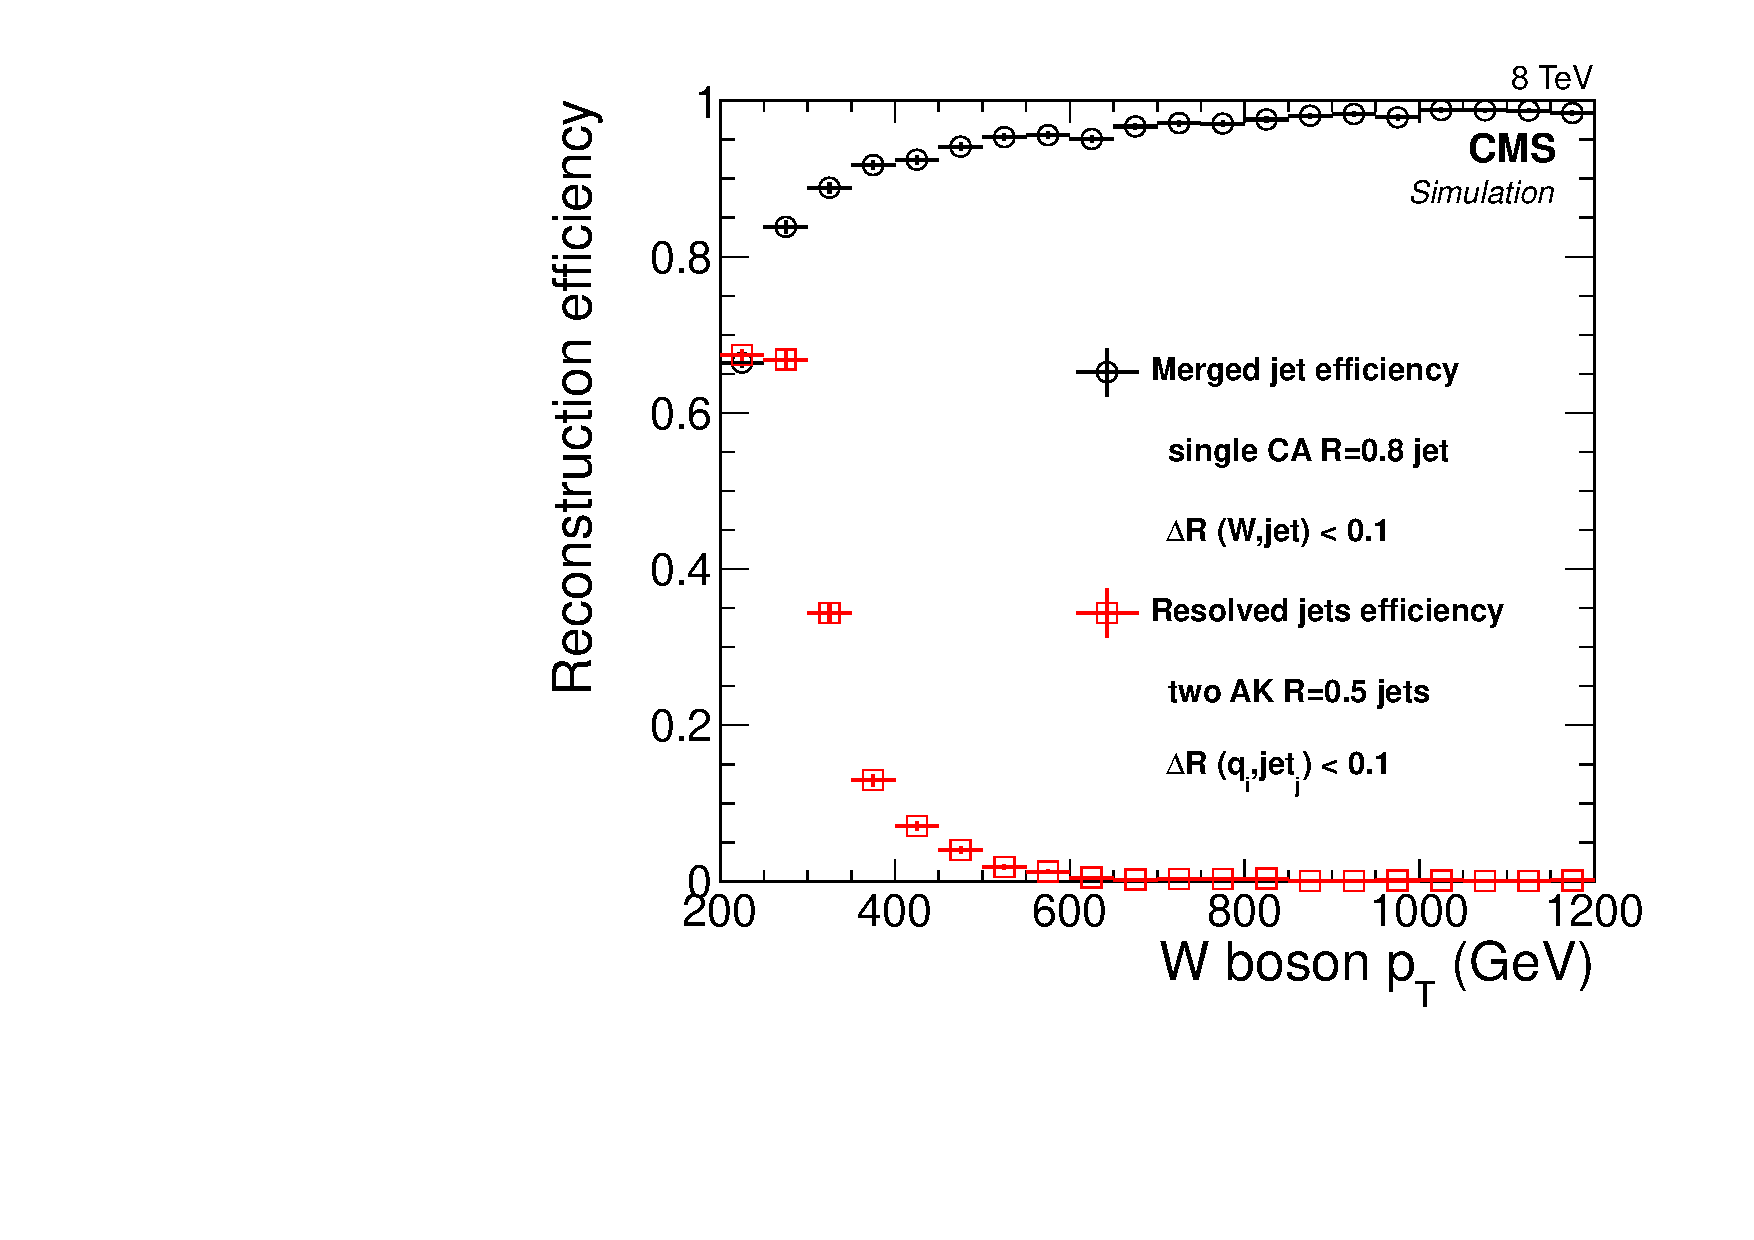
\includegraphics[width=3.5 in]{Analysis/EventSelection/ca8effVsPt.pdf}
\end{center}
\caption{Efficiency to reconstruct a Cambridge-Aachen jet with a cone size of 0.8 (CA8) within $\Delta R < 0.1$ of a generated W boson, and the efficiency to reconstruct two anit-$k_t$ jets with a 0.5 cone size (AK5) within $\Delta R < 0.1$ of the generated quarks from the W boson, as a function of the $p_{T}$ of the W boson~\cite{BoostedWid} Here, the fatjet is clustered with the CA algorithm but the reconstruction efficiency does not depend on the jet algorithm that is used to cluster the jets. Also, the same trend occurs for reconstructed Higgs bosons with large $p_{T}$, although the turnover in efficiency between a single fatjet and two smaller jets takes place at a slightly higher $p_{T}$ due to the higher mass of the Higgs compared to the W boson.}
\label{fig:BoostedRecoEff}
\end{figure}

Each jet is also required to pass the tight jet identification requirements provided by the CMS JetMET physics analysis group. These selections require a jet to have a neutral hadron fraction $< 0.9$, a neutral EM fraction $< 0.9$, a muon fraction $< 0.8$, a charged hadron fraction $> 0$, a charged EM fraction $< 0.9$, and more than 1 constituent. The hadron fraction is the percentage of jet constituents taken from HCAL hits, the EM fraction is the percentage of jet constituents taken from ECAL hits, and the muon fraction is the percentage of constituents taken from the muon detector. These requirements are summarized in Table~\ref{tab:tightjetid}.

\begin{table}[h!]
  \begin{center}
    \begin{tabular}{l r}
    \hline
    \hline
    Variable &  Cut \\
    \hline
    Neutral Hadron Fraction & $<0.90$  \\
    Neutral EM Fraction     & $<0.90$  \\
    Number of Constituents  & $>1$     \\
    Muon Fraction           & $<0.8$   \\
    Charged Hadron Fraction & $>0$     \\
    Charged Multiplicity    & $>0$     \\
    Charged EM Fraction     & $< 0.90$ \\
    \hline
    \hline
    \end{tabular}
   \caption{Tight jet identification quality criteria used in the analysis.\label{tab:tightjetid}}
  \end{center}
\end{table}

\subsubsection{Candidate Higgs Selection}

To further reduce the large amount of QCD background, a set of jet requirements is applied that distinguish a quark/gluon-initiated jet (QCD jet) from a Higgs jet. Jets that originate from a Higgs have different phenomenological properties than QCD jets and these properties can be exploited by comparing the mass of the jet, the substructure of the jet, and the flavor of the jet. 

To begin, the masses of the two leading jets can be used to suppress the multijet and $\mathrm{t\bar{t}}$ backgrounds. The jet is first groomed~\cite{JetGrooming} to mitigate the effects of initial state radiation, underlying event activity, and pileup using the soft-drop algorithm~\cite{SDMass, SoftDrop}. The soft-drop algorithm is a declustering algorithm that recursively removes soft, wide-angle radiation from a jet. The soft-drop declustering procedure begins by undoing the last step of jet clustering by breaking the jet, $j$, into two subjets, $j_{1}$ and $j_{2}$. If the subjets pass the soft-drop condition

\begin{equation}
\frac{\mathrm{min}(p_{T1},p_{T2})}{p_{T1}+p_{T2}} > z_{cut}\bigg(\frac{\Delta R_{12}}{R_{0}}\bigg)^{\beta},
\end{equation}

\noindent
then the original jet is kept as the final jet. Otherwise, the subjet with the lowest $p_{T}$ is thrown away, $j$ is redefined as the remaining subjet, and the declustering is repeated until the soft-drop condition is satisfied. Here, $p_{Ti}$ is the transverse momenta of the two constituents, $\Delta R_{12}$ is the angular distance between the constituents, $R_{0}$ is the size of the jet, $z_{cut}$ is the soft-drop threshold, and $\beta$ is an angular component where $\beta\rightarrow\infty$ returns an ungroomed jet. In this analysis, $z_{cut}$ is set to $0.1$ and $\beta = 0$. 

The groomed jet is used to calculate the soft-drop jet mass and dedicated mass corrections, which are derived from data and simulation in a region enriched in $\mathrm{t\bar{t}}$ events with merged $W\rightarrow q\bar{q}$ decays~\cite{SDCorr}, are applied in a two step procedure. First, a weight to account for a $p_{T}$ dependent soft-drop jet mass shift introduced at generator level is computed. Then an additional weight, to account for any residual $p_{T}$ and $\eta$ dependence, is calculated based on the difference between the reconstructed and the generated soft-drop mass. These corrections applied to a Higgs jet yield a mass stable with $p_{T}$ and number of pileup interactions, peaking around 120 GeV. The difference of ${\sim}5$ GeV relative to the nominal Higgs mass is related to the presence of neutrinos produced by the semi-leptonic decays of B mesons. For quark/gluon-initiated jets, the removal of underlying events pushes the jet mass to lower values and the distribution has much smoother behavior than ungroomed jets, as seen in Figure~\ref{fig:QCDSDMass}. In this analysis, the soft-drop masses of each jet are required to fall within the range $105-135$ GeV, which corresponds to an efficiency of about $60-70\%$ depending on the mass of the $X$ resonance. 

\begin{figure}[h!]
\begin{center}
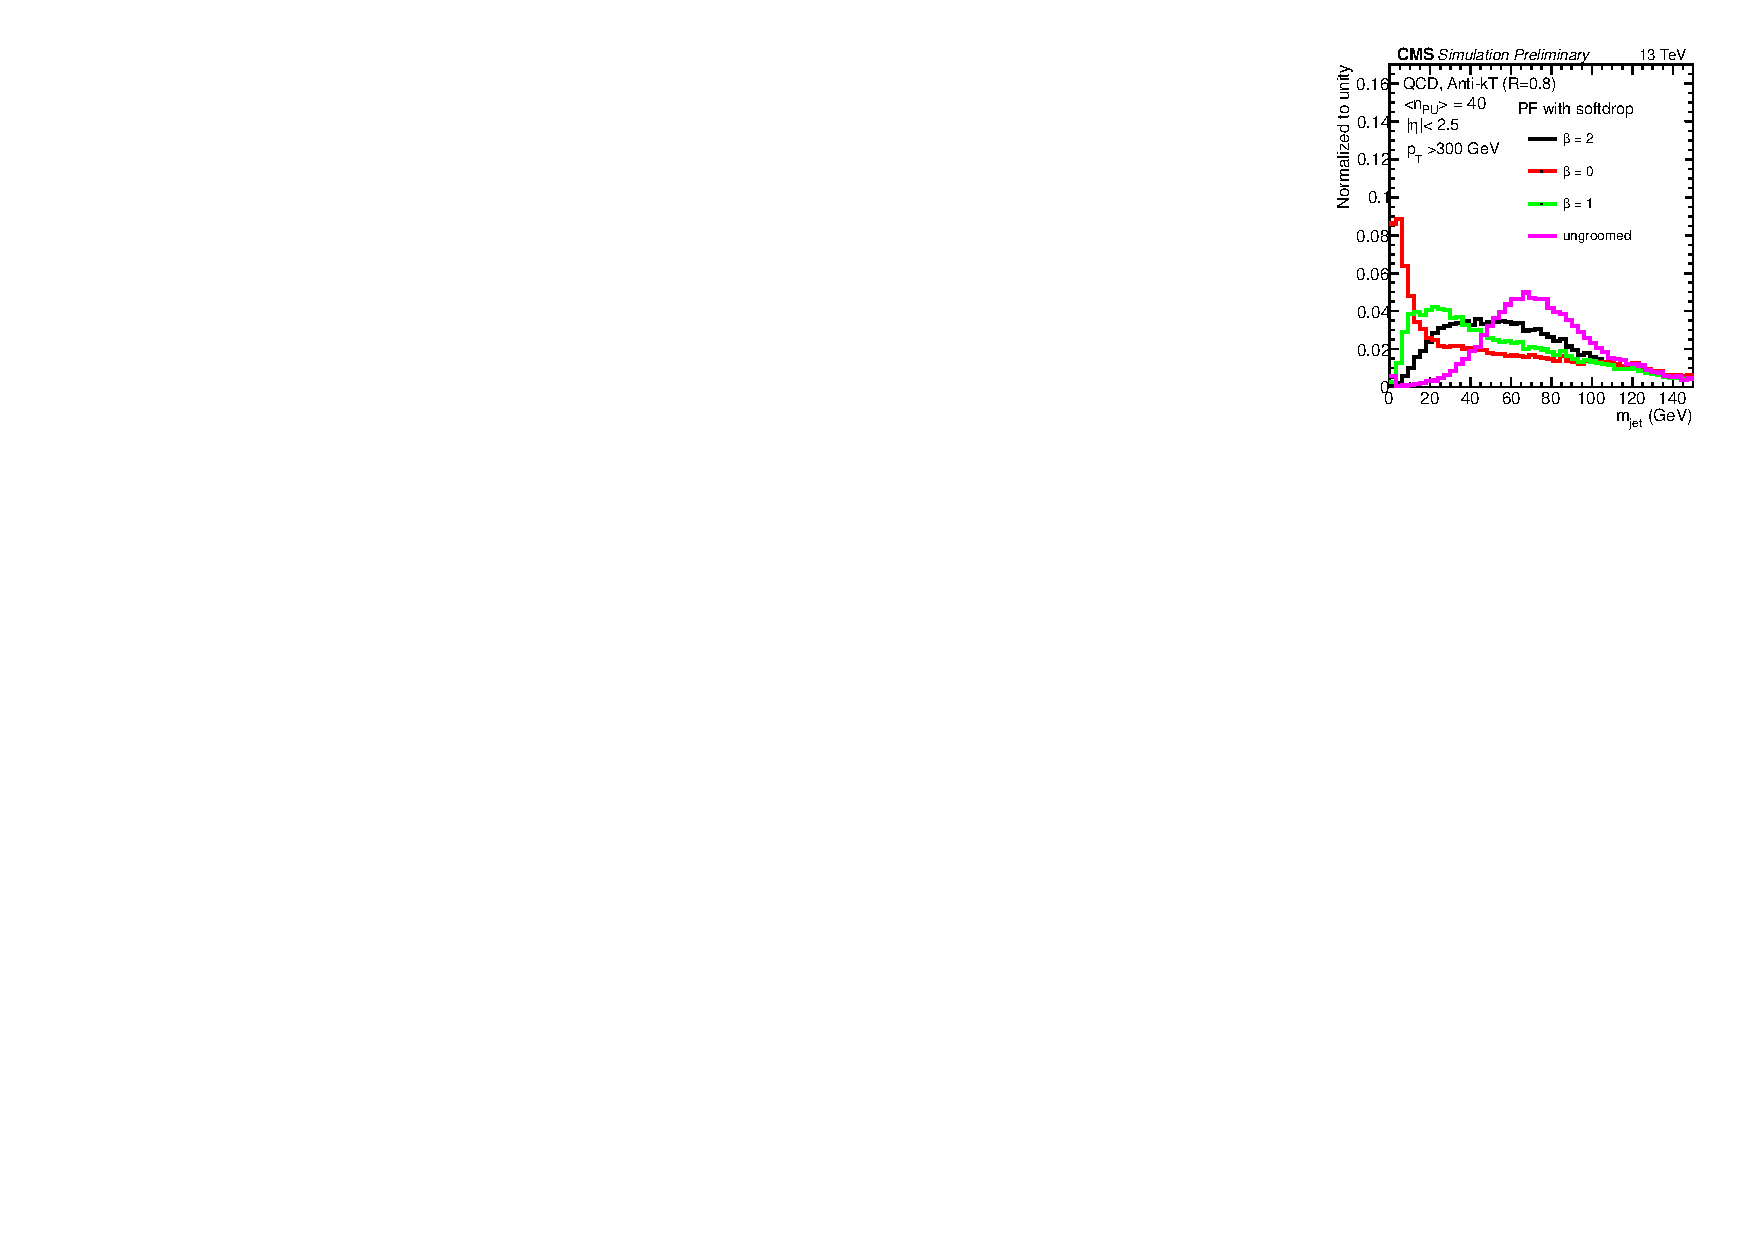
\includegraphics[width=3 in]{Analysis/EventSelection/QCD_AK8JetMass.pdf}
\end{center}
\caption{Jet mass distributions of simulated QCD jets with $p_{T}>300$ GeV for jets with different soft-drop parameters. The ungroomed jet mass is also shown~\cite{QCDJetMass}.}
\label{fig:QCDSDMass}
\end{figure}

%Dedicated jet mass corrections are applied to the soft-drop mass in two steps.

%in order to remove residual dependence on the jet $p_{T}$, and to match the jet mass scale and resolution observed in data. 

%The groomed jet is used to calculate the soft-drop jet mass, which peaks at the Higgs boson mass for signal events and reduces the mass of background QCD jets. However, a dedicated jet mass correction~\cite{SDCorr} must be applied to these groomed jets, similar to the jet energy corrections that were described in the previous section. This is a two step correction that is derived from data and simulation in a region enriched with $\mathrm{t\bar{t}}$ events with merged $W\rightarrow q\bar{q}$ decays. The first correction accounts for a $p_{T}$ dependent soft-drop jet mass shift introduced at the generator level. Then an additional weight, to account for any residual $p_{T}$ and $\eta$ dependence, is calculated based on the difference between the reconstructed and the generated soft-drop mass after the gen correction is applied. These corrections applied to a Higgs jet yield a mass stable with $p_{T}$ and number of true interactions, peaking around the Higgs mass.

An additional observable that can distinguish QCD jets from Higgs jets is the substructure of a jet. A Higgs jet has two prongs of energy within it corresponding to each of the b quarks, whereas a QCD jet has energy uniformly distributed throughout the jet cone. The algorithm used to quantify the degree to which a jet's constituents can be arranged in $N$ subjets is called ``N-subjettiness''~\cite{BoostTop}, or $\tau_{N}$, where

\begin{equation}
\tau_{N} = \frac{1}{\sum_{k}p_{T,k}R_{0}}\sum_{k}p_{T,k}\mathrm{min}(\Delta R_{1,k},\Delta R_{2,k}...,\Delta R_{N,k}).
\end{equation}

\noindent
Here, $k$ runs over the constituents of a jet, $\Delta R_{j,k}$ is the angular distance between a subjet axis $j$ and a constituent $k$, and $R_{0}$ is the size of the jet. The subjet axes are identified using the exclusive-$k_{t}$ clustering algorithm~\cite{kTCluster, kTCluster2}. Jets with $\tau_{N}=0$ are consistent with a jet containing $N$ or fewer subjets since all of their constituents are aligned with the subjet axes. 

To distinguish jets containing two subjets from jets with a single subjet, the ratio $\tau_{21}=\tau_{2}/\tau_{1}$ has been shown to have the most discrimination power~\cite{BoostNsub}. Figure~\ref{fig:QCDtau21} illustrates that small values of $\tau_{21}$ indicate a jet is consistent with containing two subjets. Both of the jets in this analysis are required to have $\tau_{21} < 0.55$ which is the loose working point supported by the CMS JetMET Algorithms and Reconstruction POG and was chosen because tighter working points caused a reduction in expected sensitivity. The $\tau_{21}$ selection has a jet $p_{T}$-dependent signal efficiency of $50-70\%$, before applying the soft-drop mass requirement.

\begin{figure}[h!]
\begin{center}
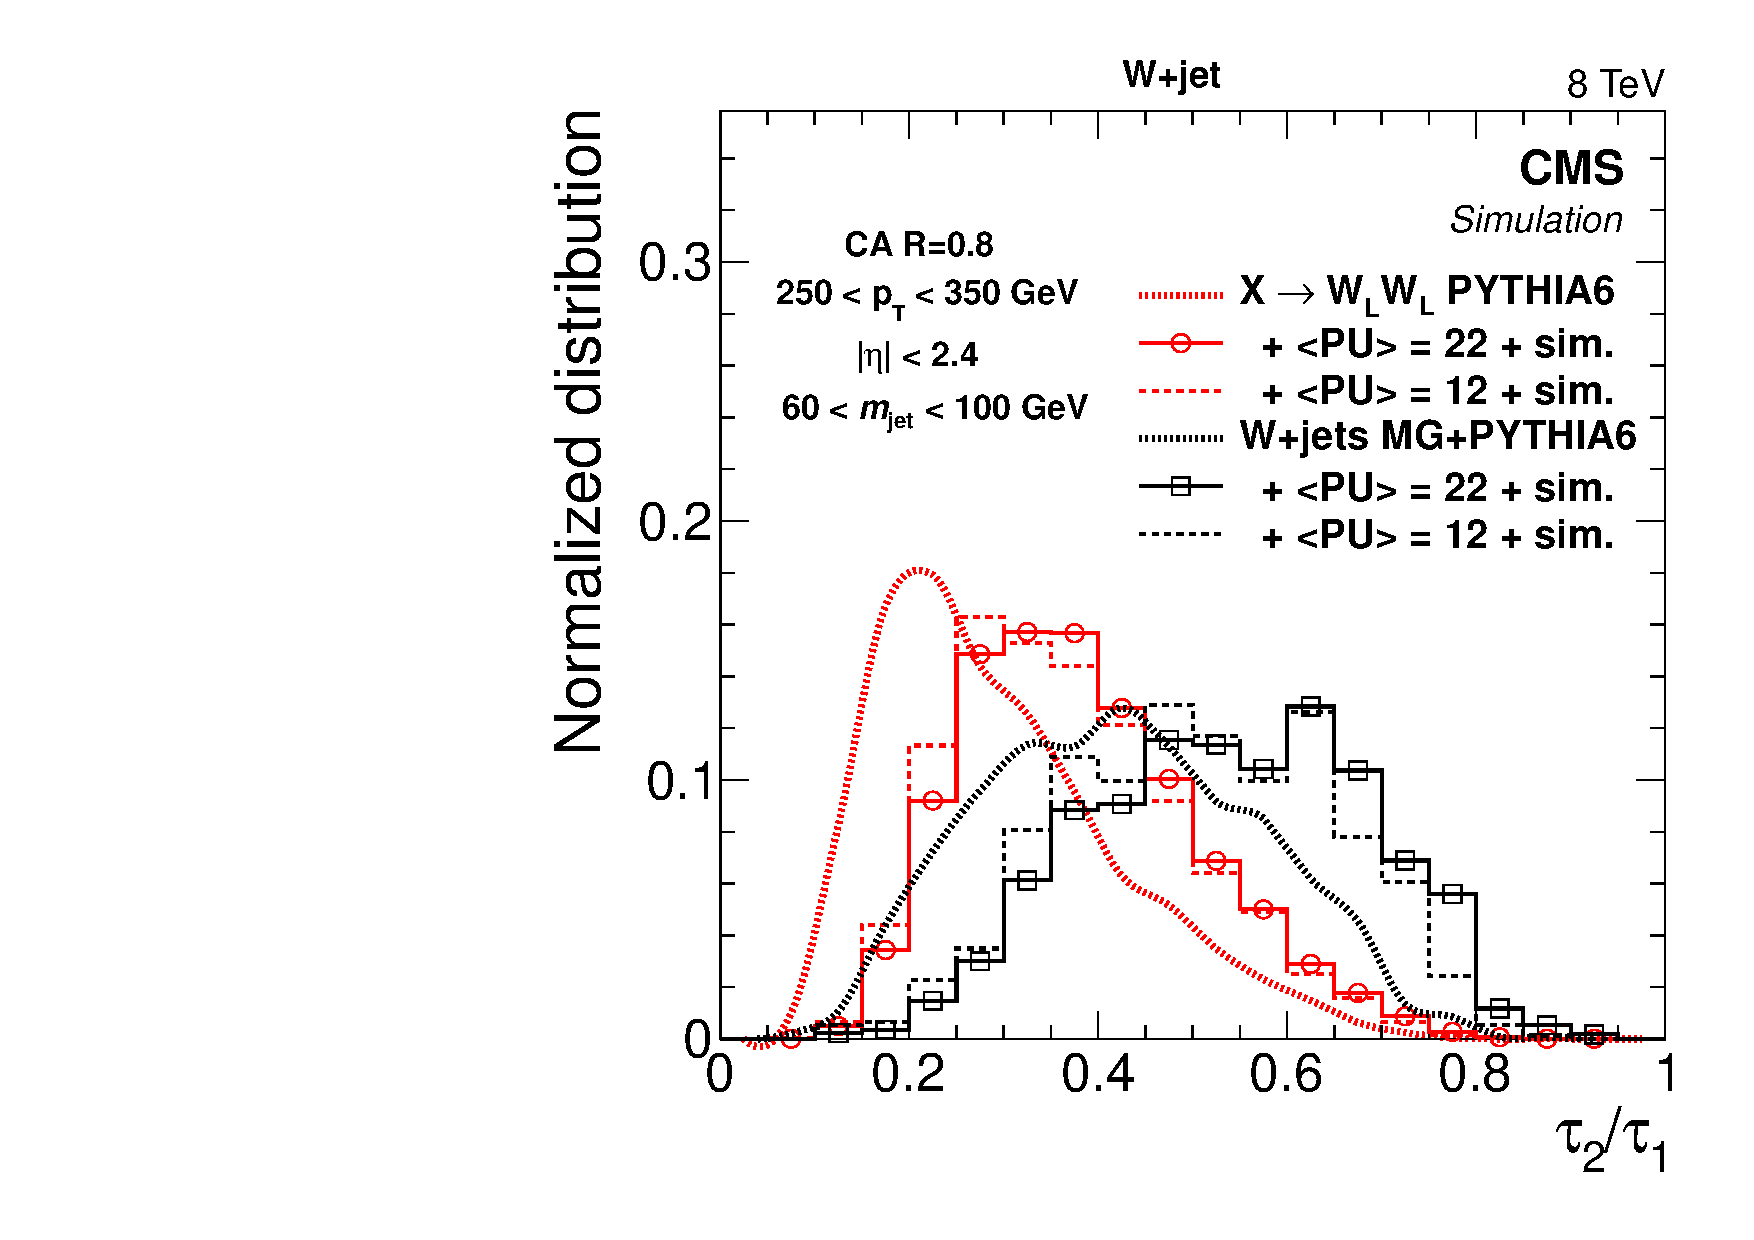
\includegraphics[width=3 in]{Analysis/EventSelection/tau2tau1_afterMass.pdf}
\end{center}
\caption{Distribution of $\tau_{2}/\tau_{1}$ in simulated samples of highly boosted W bosons and inclusive QCD jets after a jet mass selection of $60<m_{jet}<100$ GeV. Thick dashed lines represent the generator predictions without pileup interactions and without CMS detector simulation. The histograms are the expected distributions after full CMS simulation with pileup corresponding to an average number of 12 and 22 interactions~\cite{QCDJetMass}. Here, the W bosons decay to a pair of quarks, but the $\tau_{21}$ distribution is very similar for Higgs bosons decaying to a pair of b quarks.}
\label{fig:QCDtau21}
\end{figure}

Finally, the main method to suppress multijet background is through b tagging and since a Higgs jet is expected to contain two b quarks, the dedicated ``double-b tagger'' algorithm~\cite{DoubleB} is used. Due to the long decay time of a b quark, there are secondary vertices (SV) within a Higgs jet corresponding to each of the b quarks. These secondary vertices are then associated to a subjet axis, which are defined in the N-subjettiness observables, to form a two-SV system. The secondary vertices, reconstructed tracks, and information from the two-SV system are used as input to the multivariate tagging discriminator with an output between $-1$ and $1$, where a higher value indicates a greater probability for the jet to contain a $\mathrm{b\bar{b}}$ pair, as shown in Figure~\ref{fig:DoubleB}. 

\begin{figure}[h!]
\begin{center}
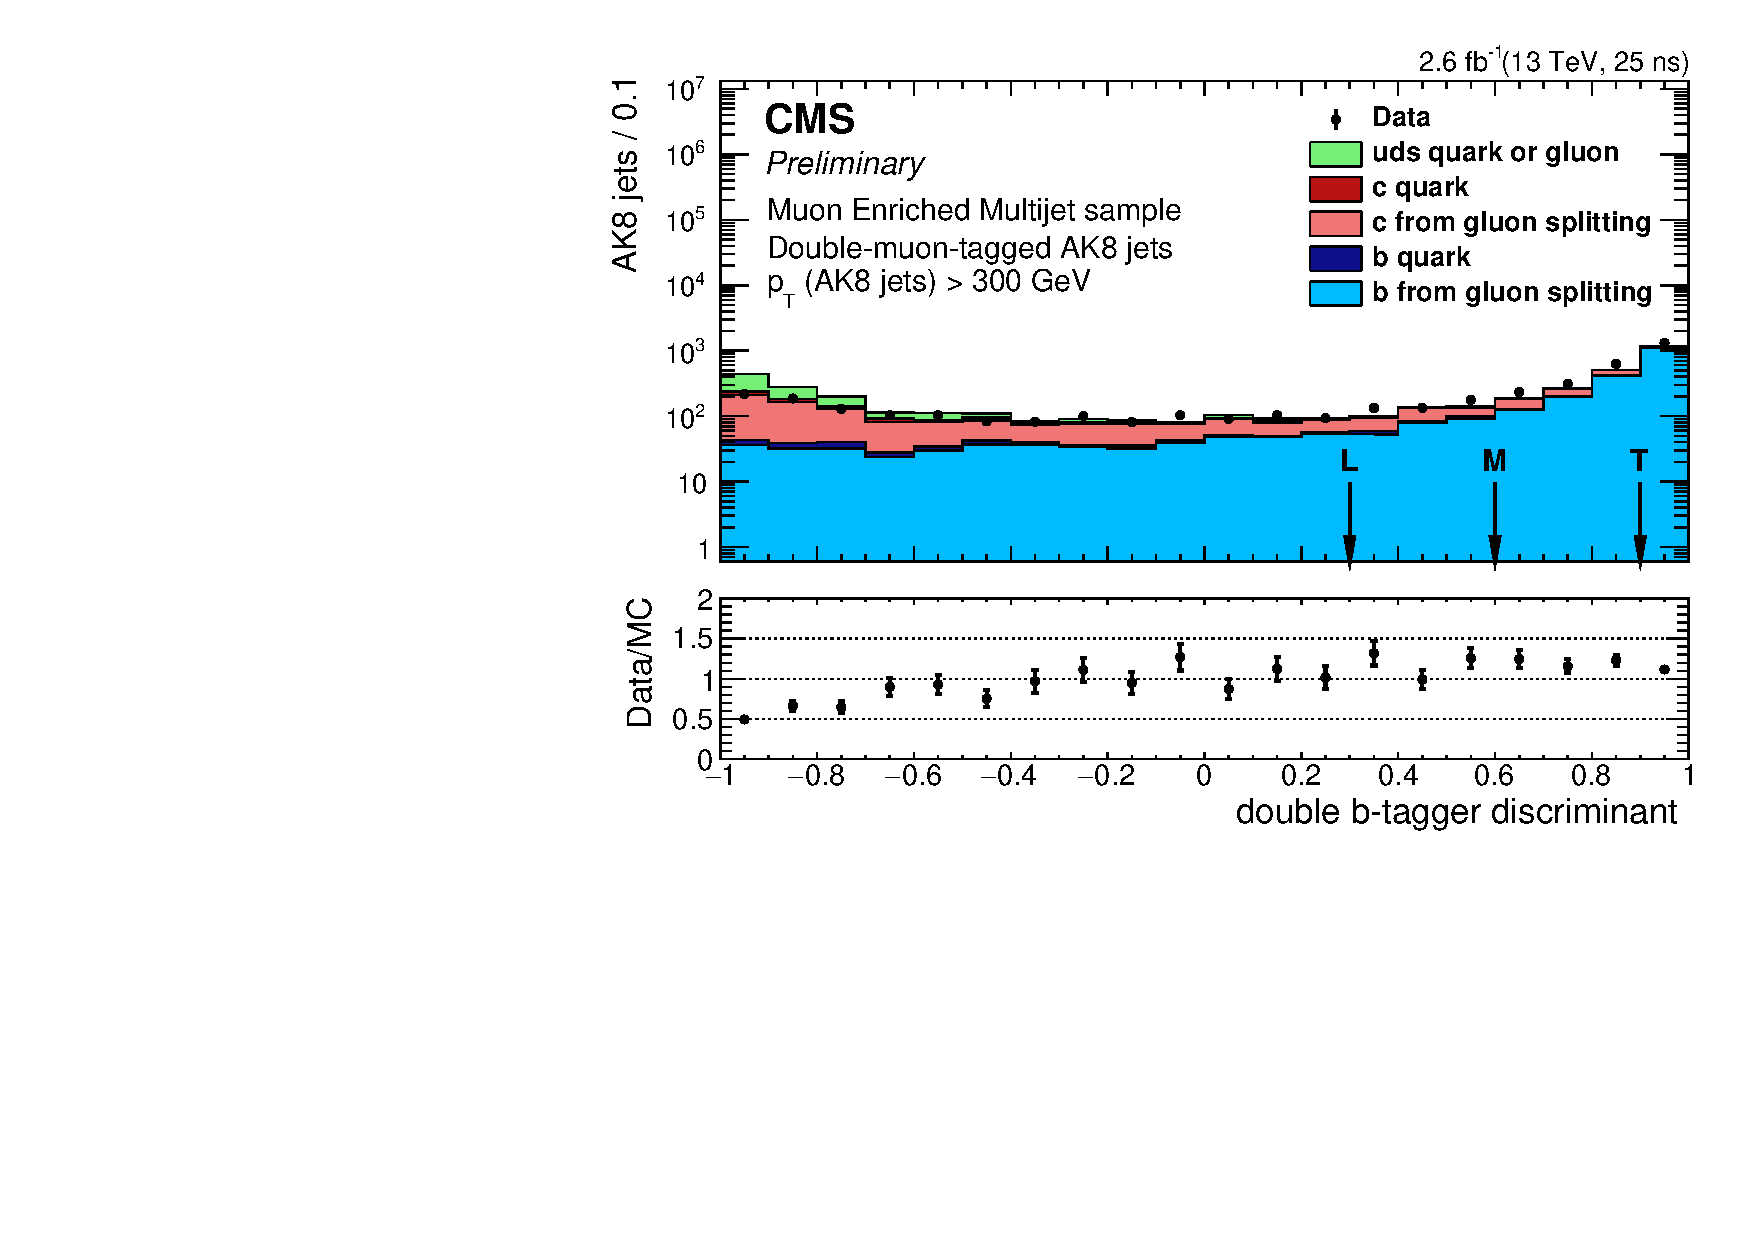
\includegraphics[width=3 in]{Analysis/EventSelection/CMS-PAS-BTV-15-002_Figure_006.pdf}
\end{center}
\caption{Double-b tagger discriminant distribution in data and simulated samples for the double-muon tagged jets selection. Simulated events are normalized to the yield observed in data. The loose, medium and tight operating points are also reported. The bottom panel shows the ratio of the number of events observed in data to that of the MC prediction~\cite{DoubleB}.}
\label{fig:DoubleB}
\end{figure}

The double-b discriminator working points that are supported by the CMS BTagging and Vertex POG are loose (``L'', $>0.3$), medium (``M'', $>0.6$), and tight (``T'', $>0.8$) corresponding to signal efficiencies of $80\%$, $65\%$, and $30\%$, respectively. The working points used in this analysis were optimized separately for low and high $p_{T}$ jets by applying the full event selection and running the analysis framework on data to calculate the $95\%$ confidence level expected upper limits on the production cross section $\sigma(\mathrm{pp}\rightarrow \mathrm{X})B(\mathrm{X}\rightarrow\mathrm{HH}\rightarrow\mathrm{b\bar{b}b\bar{b}})$ as a function of bulk graviton mass. The following combinations of double-b tagger working points were investigated:

\begin{itemize}
\item TT: both jets pass the tight selection;
\item TM: one jet passes the tight selection and one passes the medium selection;
\item TL: one jet pass the tight selection and one passes the loose selection;
\item MM: both jets pass the medium selection;
\item ML: one jet passes the medium selection and one passes the loose selection;
\item LL: both jets pass the loose selection.
\end{itemize}

\noindent
Figure~\ref{fig:DoubleBoptimization} compares the expected limits for these combinations across a wide range of bulk graviton masses. The optimal choice results in the tight working point for low and medium $p_{T}$ jets while the loose working point is optimal for high $p_{T}$ jets. Therefore, our events were classified into two orthogonal categories, TT and LL. These categories are kept orthogonal by requiring at least one jet in the LL category to fail the tight working point. The backgrounds are estimated separately for each category, and the combination of the likelihoods for the TT and LL categories gives the optimal signal sensitivity over a wide range of resonance masses, according to studies performed using simulated signal and multijet samples. The TT category has a good background rejection for $m_{X} < 2000$ GeV while at higher resonance masses, where the background is small, the LL category provides better signal sensitivity.

%\begin{itemize}
%\item TT: both jets pass the tight working point
%\item LL: both jets pass the loose working point and at least one jet failing the tight working point
%\end{itemize}



%The working points used in this analysis were optimized separately for low and high $p_{T}$ jets based on expected sensitivity. The optimal choice results in the tight working point for low and medium $p_{T}$ jets while the loose working point is optimal for high $p_{T}$ jets. This optimization was done using a full event selection and expected limits based on data. 

\begin{figure}[h!]
\begin{center}
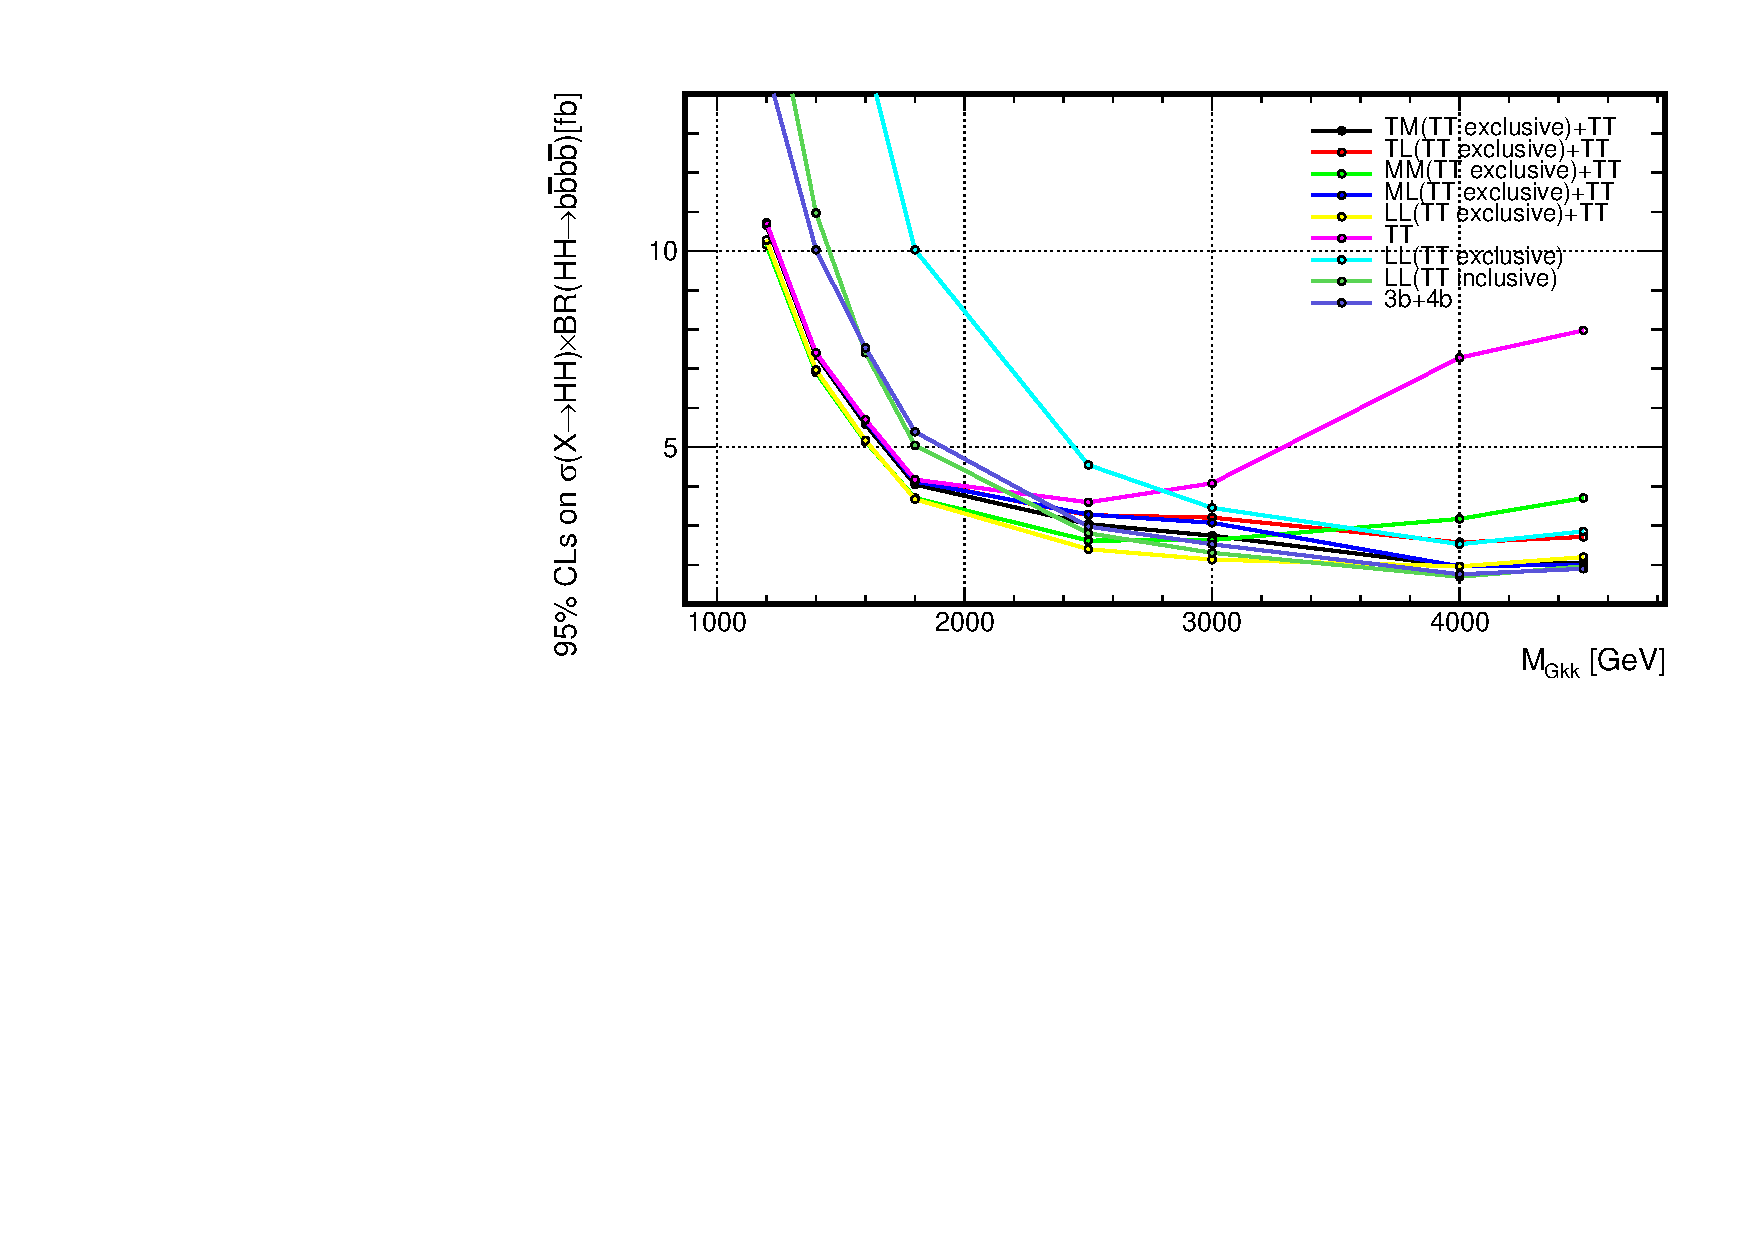
\includegraphics[width=4.5 in, height=3 in]{Analysis/EventSelection/BDTLimitcombine.pdf}
\end{center}
\caption{The $95\%$ confidence level expected upper limits as a function of bulk graviton resonance mass for different b-tagging categories. Note, when combining the TT category with other categories, the TT events are excluded. The limits using a subjet single b tagging selection (3b $+$ 4b) are also shown for comparison. }
\label{fig:DoubleBoptimization}
\end{figure}

\subsubsection{Jet $\eta$ Separation}

For multijet background events, the two candidate Higgs jets have a large separation in $\eta$. In contrast, the signal events are characterized by a small separation of the two leading $p_{T}$ jets in $\eta$. To determine the optimal value for the $|\Delta\eta(\mathrm{j}_{1}, \mathrm{j}_{2})|$ selection, the value of $\frac{\epsilon_{\rm signal}}{1 + \sqrt{N_{\rm bkg}}}$ was used as a figure of merit (FOM), where $\epsilon_{\rm signal}$ is the signal efficiency, and $N_{\rm bkg}$ is the number of background events passing the $|\Delta\eta(\mathrm{j}_{1}, \mathrm{j}_{2})|$ selection criteria. The results are shown in Figure~\ref{fig:app_DetaSig_BG} and~\ref{fig:app_DetaSig_Radion} for different bulk graviton and radion masses, respectively. Below a resonance mass of 2 TeV, the FOM favors $|\Delta\eta(\mathrm{j}_{1}, \mathrm{j}_{2})| < 1.1-1.3$, while for higher masses, a looser $|\Delta\eta(\mathrm{j}_{1}, \mathrm{j}_{2})|$ selection is optimal, given that the background levels fall steeply. The $\eta$ separation between the Higgs bosons in the resonance decay varies depending on the spin of the resonance, where the decay products from a graviton have a smaller separation than the decay products from a radion of the same mass. However, the $|\Delta\eta(\mathrm{j}_{1}, \mathrm{j}_{2})|$ selection changes the trigger turn-on, and hence the background shapes would differ for low and high mass searches, or radion and graviton searches, if different trigger turn-ons are used. Therefore, a single selection of $|\Delta\eta(\mathrm{j}_{1}, \mathrm{j}_{2})| < 1.3$ for all masses for both the bulk graviton and the radion is used.

\begin{figure}[h!]
  \centering
    \includegraphics[width=0.45\textwidth]{Analysis/EventSelection//BulkGrav/dEtaLL.pdf}
    \includegraphics[width=0.45\textwidth]{Analysis/EventSelection//BulkGrav/dEtaTT.pdf}
  \caption{The significance, $\frac{\epsilon_{\rm signal}}{1 + \sqrt{N_{\rm bkg}}}$, of the $|\Delta\eta(\mathrm{j}_{1}, \mathrm{j}_{2})|$ selection for various selection values as a function of the bulk graviton signal mass for the LL category (left) and the TT category (right).} \label{fig:app_DetaSig_BG}
\end{figure}

\begin{figure}[h!]
  \centering
    \includegraphics[width=0.45\textwidth]{Analysis/EventSelection//Radion/dEtaLL.pdf}
    \includegraphics[width=0.45\textwidth]{Analysis/EventSelection//Radion/dEtaTT.pdf}
  \caption{The significance, $\frac{\epsilon_{\rm signal}}{1 + \sqrt{N_{\rm bkg}}}$, of the $|\Delta\eta(\mathrm{j}_{1}, \mathrm{j}_{2})|$ selection for various selection values as a function of the radion signal mass for the LL category (left) and the TT category (right).} \label{fig:app_DetaSig_Radion}
\end{figure}


\subsubsection{Di-jet Mass}
\label{sec:DijetMass}

The di-jet mass of the leading two Higgs jets in the event correspond to the invariant mass of the resonance searched for. However, it is well known that techniques such as a kinematic fit that constrains the mass of each Higgs candidate to the mass of the Higgs, $m_{H}$, improves the resonance resolution and ultimately the sensitivity~\cite{CMS-PAS-B2G-16-008}. For this analysis, the groomed and ungroomed Higgs candidate masses constrained by $m_{H}$ were considered to improve the resolution of $m_{jj}$. It was found that the ``reduced di-jet invariant mass,''

\begin{equation}
m_{jj}^{red} \equiv m_{jj} - (m_{j_{1}}-m_{H}) - (m_{j_{2}}-m_{H}),
\label{eq:Mjjs}
\end{equation}

\noindent
provides the best resolution improvement and the mean position of $m_{jj}^{red}$ remained at $\approx m_{X}$. Here, $m_{j_{1}}$ and $m_{j_{2}}$ are the soft-drop masses of the two candidate Higgs. A comparison between $m_{jj}$ and $m_{jj}^{red}$ is shown in Figure~\ref{fig:subtImp} for different resonance masses. The kinematic transformation of $m_{jj}$ corrects for fluctuations in $m_{j_{1}}$ and $m_{j_{2}}$ due to the jet mass resolution which leads to an $8-10\%$ improvement in the di-jet mass resolution. A requirement of $m_{jj}^{red}>750$ GeV is applied to events because this is the high resonance mass range that this search looked for.

\begin{figure}[h!]
\begin{center}
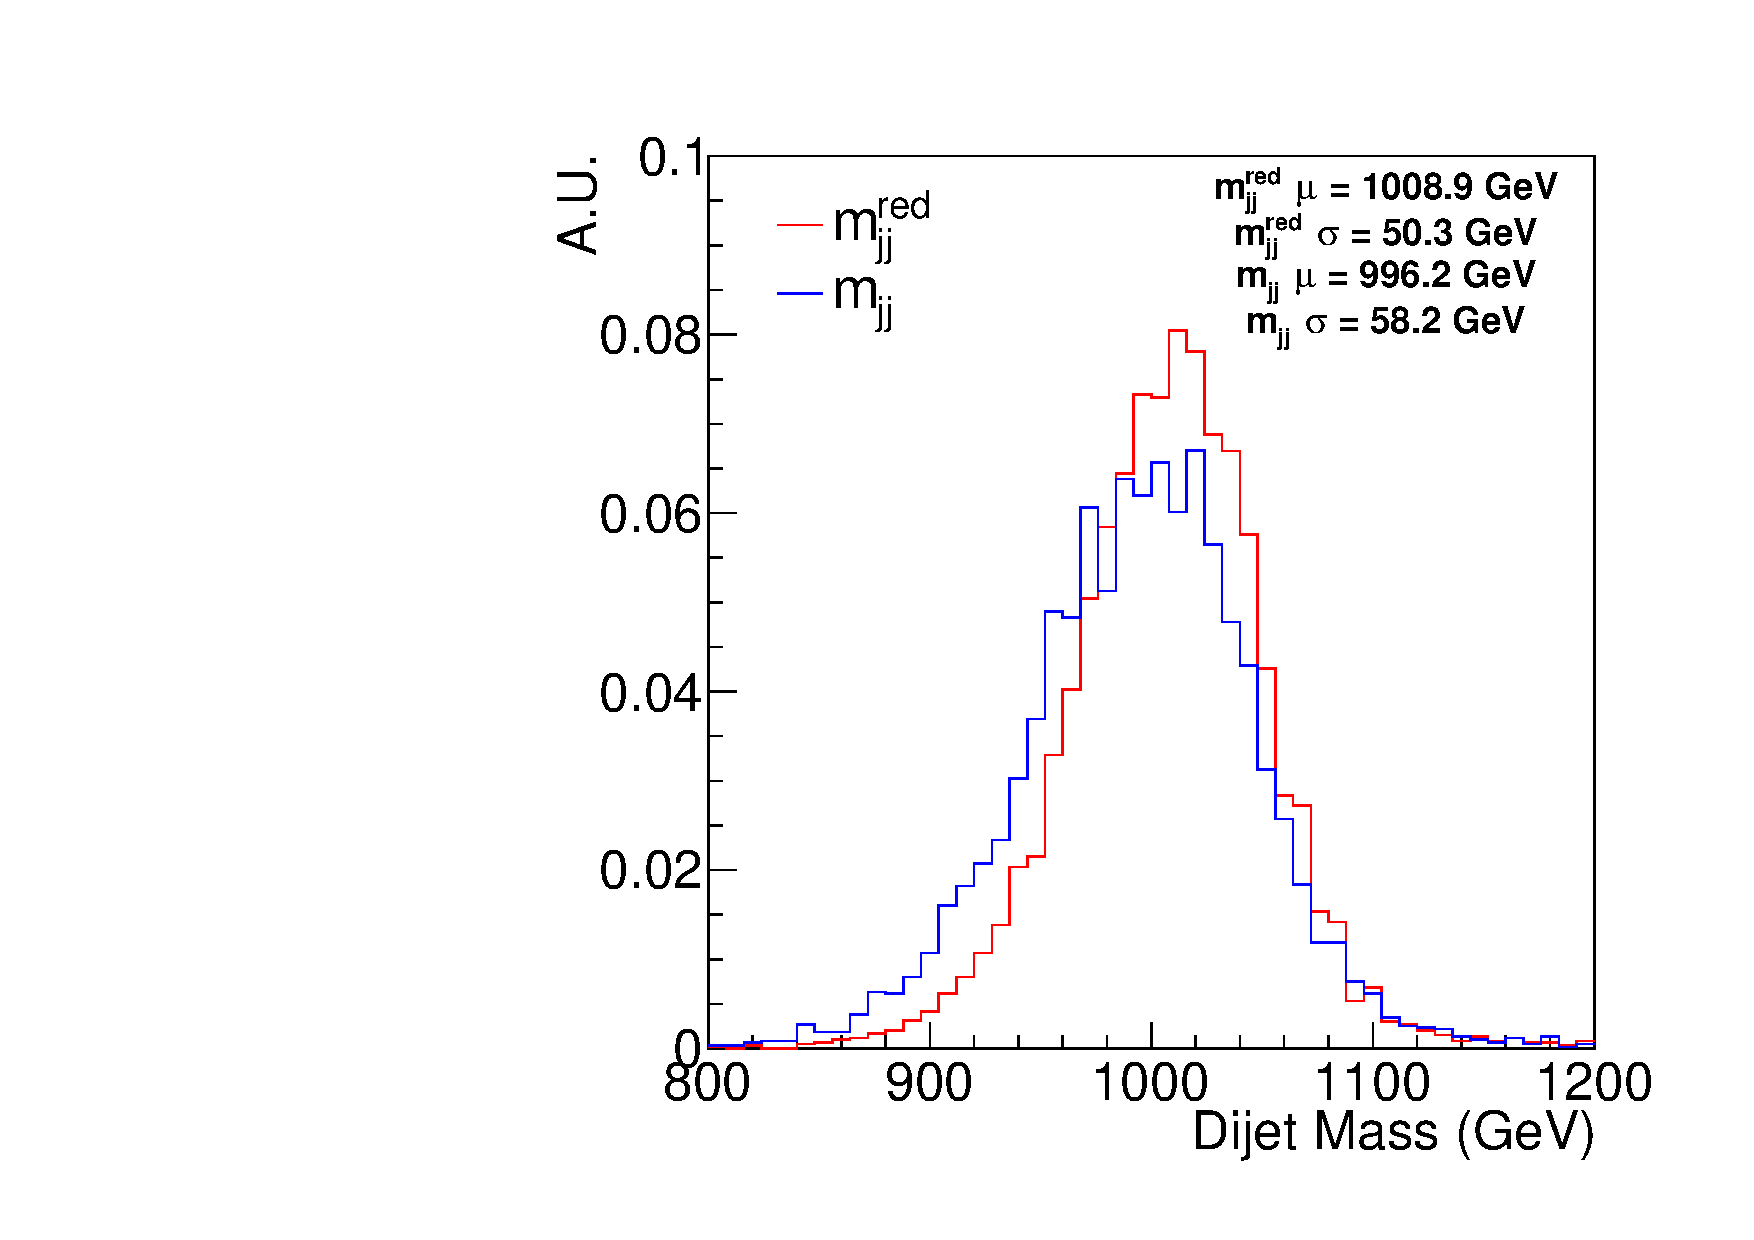
\includegraphics[scale=0.34]{Analysis/EventSelection/BulkGrav_M-1000_DijetMassCorrection.pdf}
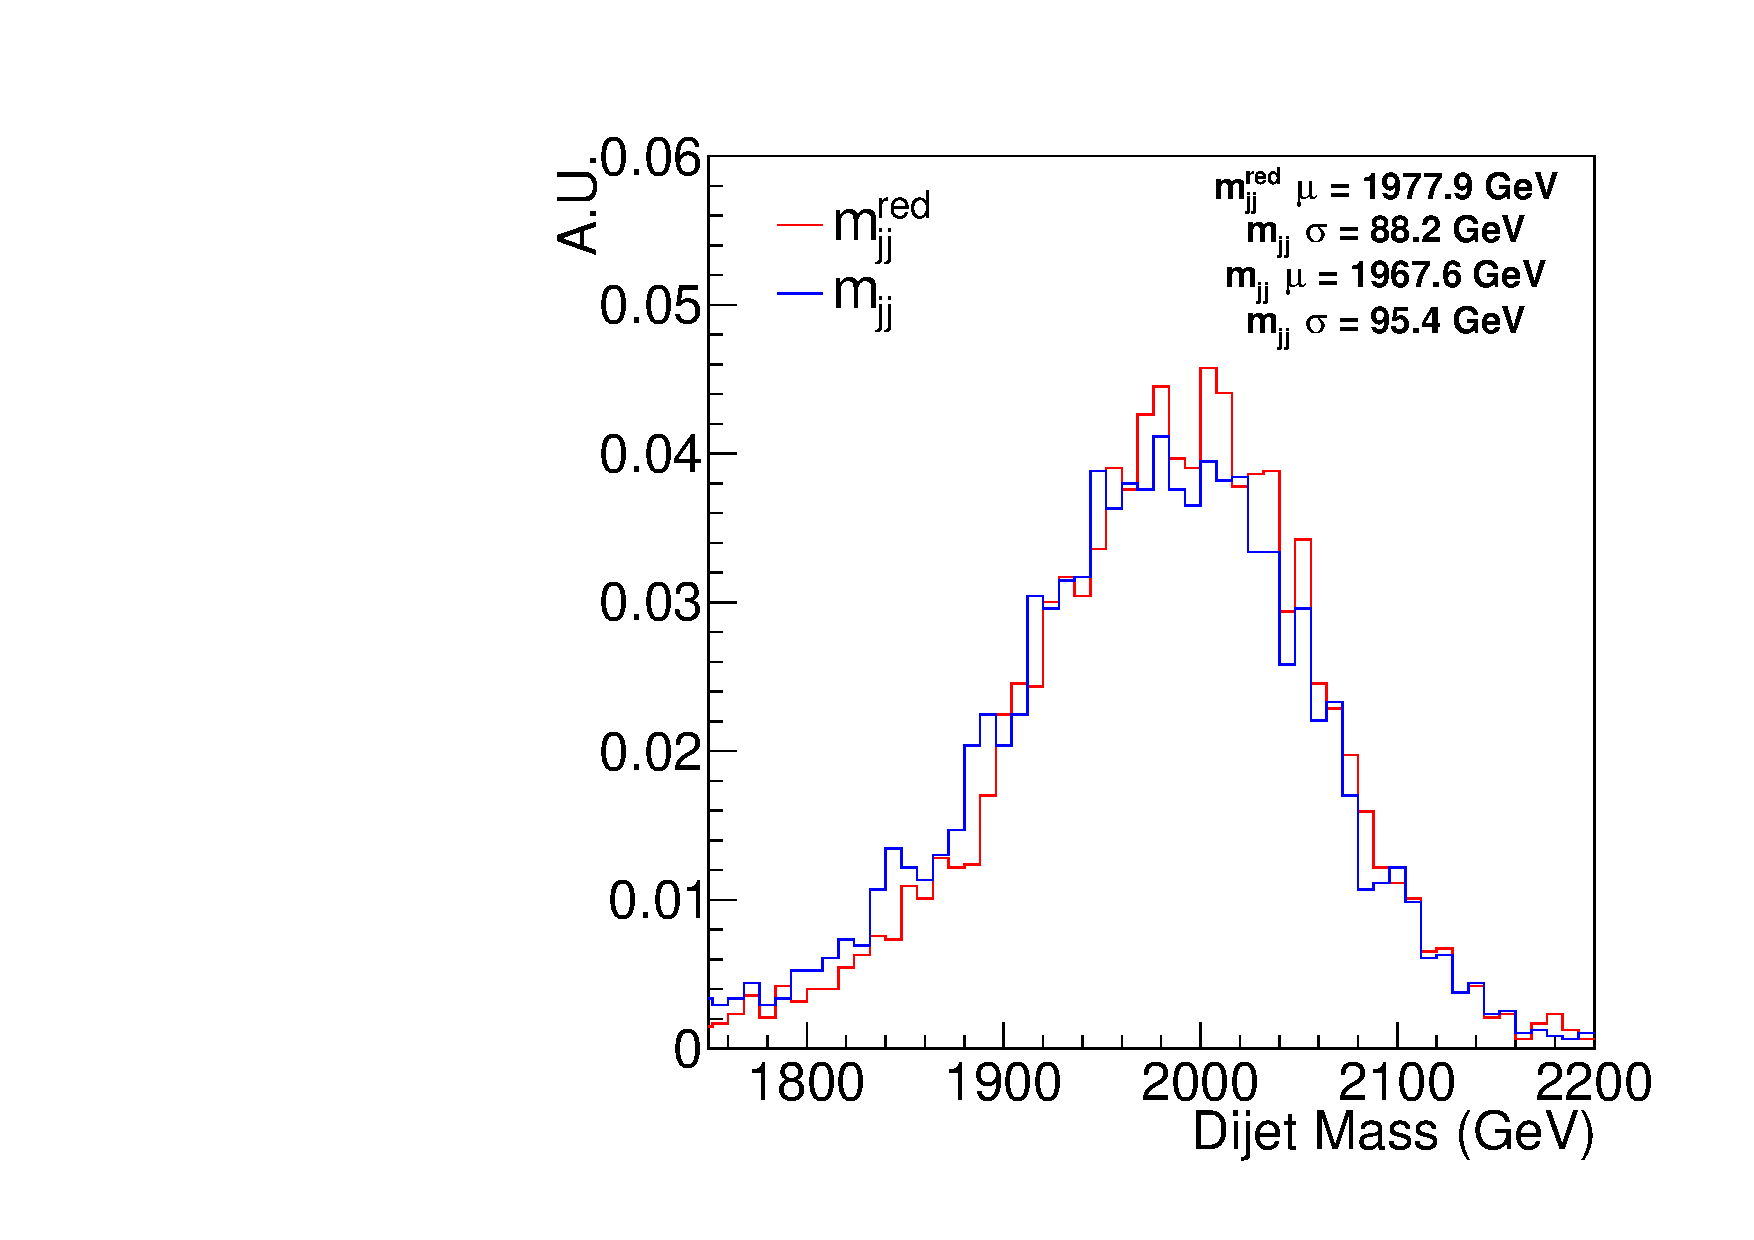
\includegraphics[scale=0.34]{Analysis/EventSelection/BulkGrav_M-2000_DijetMassCorrection.pdf}
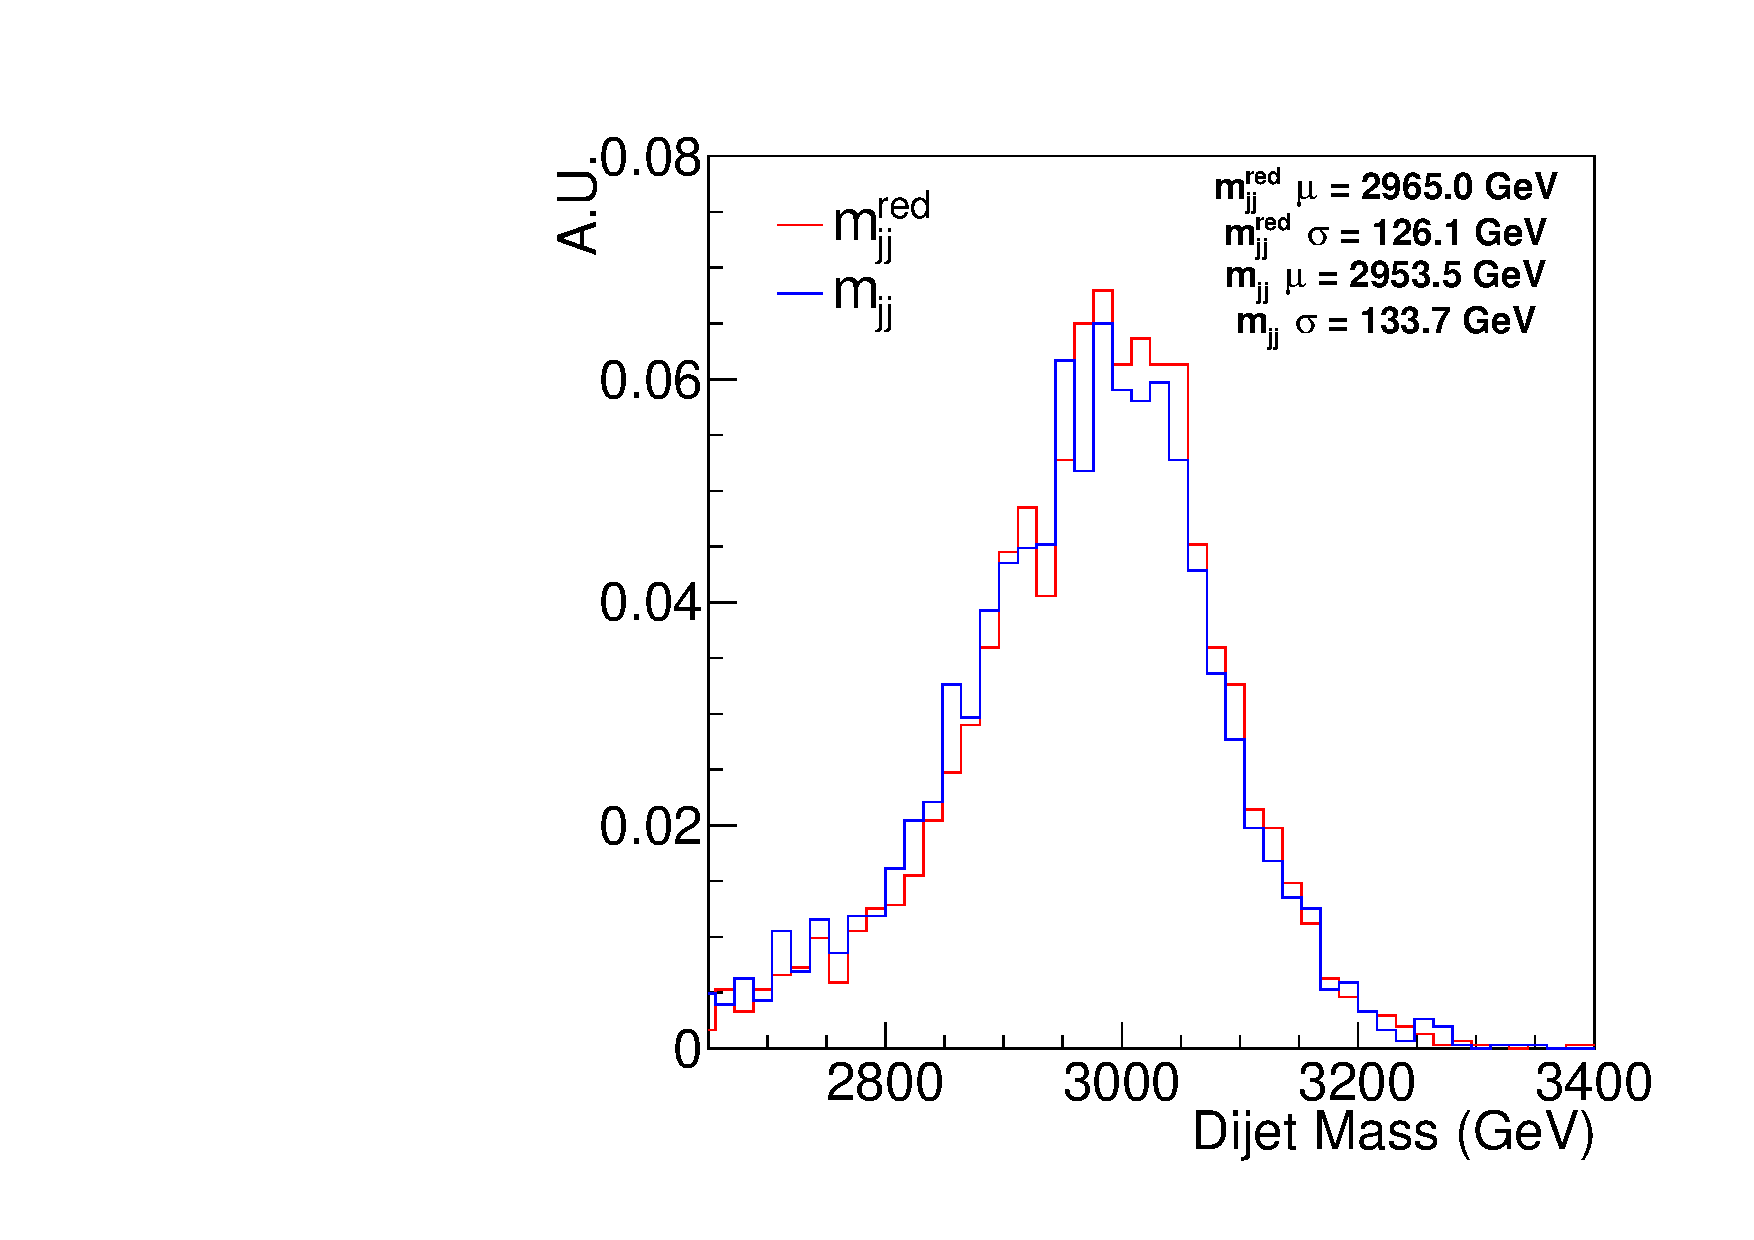
\includegraphics[scale=0.34]{Analysis/EventSelection/BulkGrav_M-3000_DijetMassCorrection.pdf}
\end{center}
\caption{The reduced di-jet mass distribution computed as described in Eqn.~\ref{eq:Mjjs} compared to the standard di-jet invariant mass for simulated signal events. The $m_{jj}^{red}$ distributions have a narrower di-jet mass distribution than the $m_{jj}$ distribtuions for each mass point. The simulated bulk graviton mass points are 1000 (top left), 2000 (top right), and 3000 (bottom) GeV.}
\label{fig:subtImp}
\end{figure}



\subsection{Full Selection}

The entire event selection is summarized in Table~\ref{tab:datamcselection}. To determine the background composition, the full event selection is applied to QCD, $\mathrm{t\bar{t}}$, and diboson simulated events. The non-QCD events comprise ${\sim}1\%$ of the total background and this can be seen in the invariant di-jet mass distribution in simulation that is shown in Figure~\ref{fig:MCcomposition}. Therefore, the background is estimated using a single technique rather than a different method for each separate process.

The cut-flow efficiency for the bulk graviton and radion samples is shown in Tables~\ref{tab:BulkGravCutFlowEff} and~\ref{tab:RadionCutFlowEff}, respectively. The full event selection efficiencies for both double-b tagger categories are also shown in Figure~\ref{fig:DoubleBEff}. The radion has a smaller efficiency than the bulk graviton because its $|\Delta\eta(\mathrm{j}_{1}, \mathrm{j}_{2})|$ distribution is considerably wider than that of a bulk graviton of the same mass, as shown in Figure~\ref{fig:eventToplogy_prebtag}. Figures~\ref{fig:eventToplogy_prebtag}$-$\ref{fig:doublesv_prebtag} compare the distributions of simulated QCD events to bulk graviton and radion signals with a mass of 1.4 and 2.5 TeV for the kinematic, jet substructure, and double-b tagger variables of the candidate Higgs jets after the full selection except for b-tagging is applied. In addition, when comparing a variable X, such as $\tau_{21}$, the selection criteria on that variable is removed. For the comparison, a signal cross section of 20 pb is assumed for each signal mass point. The simulated QCD events are subdivided into different categories based on the matched hadron flavor: jets having two B hadrons (bb) or one (b), jets having a charm hadron (c), and all other jets (light). 



%We compare the simulated distributions from QCD background and from signal after applying the pre-selection criteria in Table~\ref{tab:datamcselection}; note the b-tagging is not applied. In addition, when comparing a variable X, such as $\tau_{21}^\mathrm{PUPPI}$, the pre-selection criterion on this variable is removed. The cross sections of the QCD HT-binned MC in Section~\ref{sec:Samples} are known to be imprecise, therefore, we normalize the number of events in simulation according to the integrated luminosity of $35.9~\mathrm{fb}^{-1}$ with an additional correction factor of 0.7, which is based on the data/MC scaling observed for QCD MC in 2015 analysis, to match the event yields in MC to that in the data. Figures~\ref{fig:eventToplogy_prebtag}--\ref{fig:doublesv_prebtag} present the comparison of the distributions of the simulated QCD events for the kinematic, jet substructure, and b-tagger variables of the Higgs-jets, with those from bulk graviton with a resonance mass of 1.4, 1.8, and 2.5 TeV. For this comparison, a signal cross section of 20~pb is assumed for each signal mass point. The simulated QCD events are further subdivided into different categories based the matched hadron flavor as listed in Table~\ref{tab:qcdflavor}.


\begin{table}[h!]
\begin{center}
    \begin{tabular}{c}
    \hline
    \hline
    Selection \\
    \hline
    \texttt{PFHT650\_WideJetMJJ900DEtaJJ1p5} OR \texttt{AK8PFHT650\_TrimR0p1PT0p03Mass50} OR \\
    \texttt{AK8PFHT700\_TrimR0p1PT0p03Mass50} OR \texttt{PFHT800} OR \texttt{PFHT900} OR \\
    \texttt{AK8PFJet360\_TrimMass30} OR \texttt{AK8DiPFJet280\_200\_TrimMass30\_BTagCSV\_p20}\\
    Veto events with one medium lepton or two opposite sign loose leptons\\
    Number of good vertices $\geq 1$ \\
    Candidate Higgs jet ID passes the tight working point \\
    Candidate Higgs jet $p_{T}>300$ GeV \\
    Candidate Higgs jet $\left|\eta\right|<2.4$ \\
    $|\Delta\eta(\mathrm{j}_{1}, \mathrm{j}_{2})|<1.3$ \\
    $m_{jj}^{red}>750$ GeV \\
    Candidate Higgs jet soft-drop mass $105 < m_j <135$ GeV \\
    Candidate Higgs jet $\tau_{21}<0.55$ \\
    Candidate Higgs jet double b discriminator $> 0.3$ \\
    \hline
    \hline
    \end{tabular}
    \caption{Full selection criteria for the analysis.} \label{tab:datamcselection}
\end{center}
\end{table}

\begin{figure}[h!]
\begin{center}
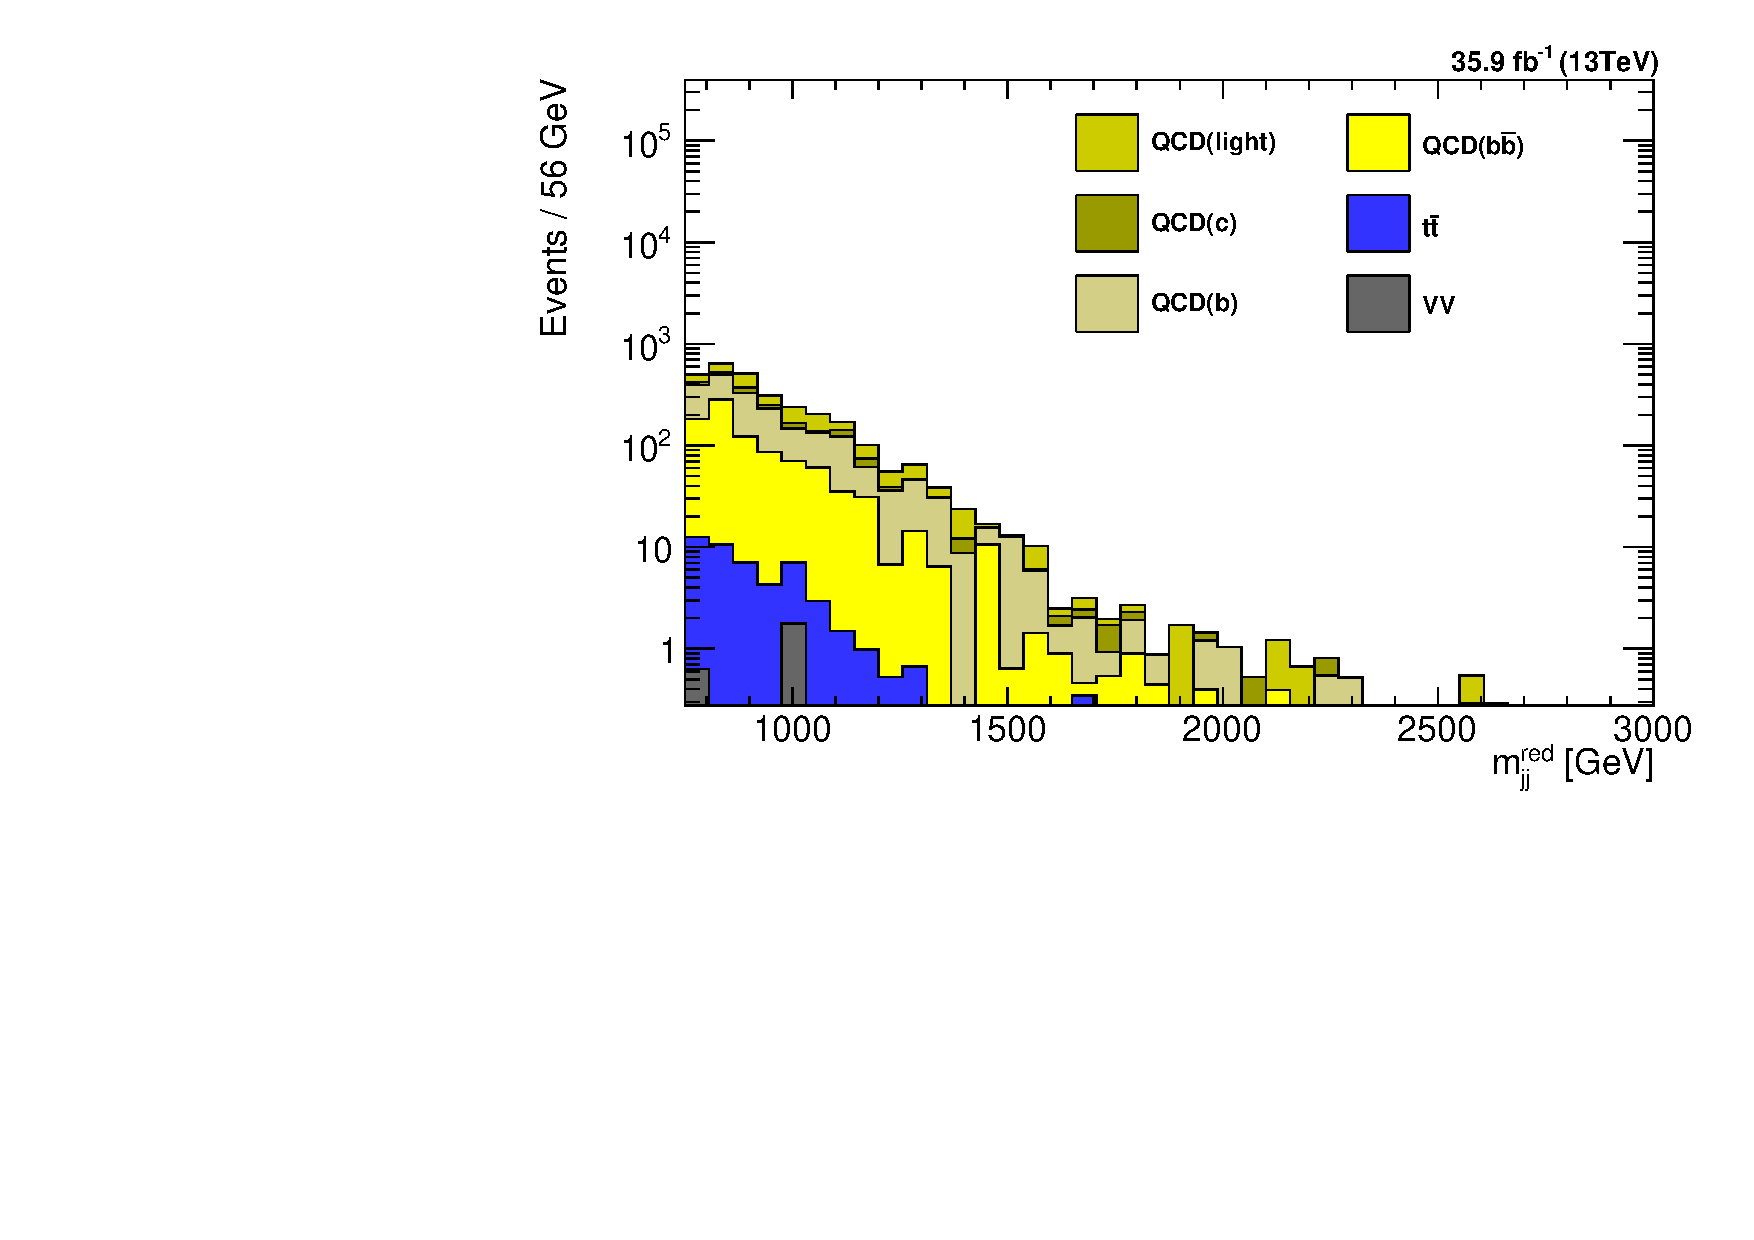
\includegraphics[width=4 in]{Analysis/EventSelection/SR_dijetmass_125_LogTrue.pdf}
\end{center}
\caption{The reduced invariant di-jet mass distribution in simulated QCD, $\mathrm{t\bar{t}}$, and diboson events after the full event selection applied. The multijet background components for the different jet flavors are shown: events containing at least one jet with two B hadrons ($\mathrm{b\bar{b}}$) or a single one (b), events containing a jet having a charm hadron (c), and all other events (light).}
\label{fig:MCcomposition}
\end{figure}

%\begin{table}[htb]
%\begin{center}
%    \begin{tabular}{c c c}
%    \hline
%    \hline
%    Label in Figures &  hadron flavor ID of AK8 jets & hadron flavor ID of sub-jets  \\
%    \hline
%    bb & 5 & 5 (both) \\
%    b & 5 & 5 (only one) \\
%    cc / c & 4 & 4 (at least one) \\
%    udsg & all remaining & all remaining \\
%    \hline
%    \hline
%    \end{tabular}
%    \caption[The categorization of simulated QCD events.]{The categorization of simulated QCD events. \label{tab:qcdflavor}}
%\end{center}
%\end{table}

\begin{table}[h!]
\center
%\begin{center}
\resizebox{\linewidth}{!}{
%\scalebox{0.6}{
\begin{tabular}{|l|c|c|c|c|c|c|c|c|c|c|}
\hline
\hline
Mass (GeV) & $\ge 2$ AK8 jets + triggers & jet $p_{T}$, $\eta$ & Tight jet ID & $\Delta\eta_{jj}$ & Lepton Veto & $\tau_{21}$ & $m_{j}$ & $m_{jj}^{red}$ & double-b tag $>0.3$ & double-b tag $>0.8$ \\ \hline
750 & 0.610 & 0.368 & 0.368 & 0.331 & 0.330 & 0.149 & 0.049 & 0.039 & 0.027 & 0.015 \\
800 & 0.758 & 0.541 & 0.541 & 0.503 & 0.502 & 0.237 & 0.080 & 0.079 & 0.057 & 0.032 \\
900 & 0.903 & 0.772 & 0.771 & 0.716 & 0.715 & 0.371 & 0.125 & 0.124 & 0.092 & 0.051 \\
1000 & 0.958 & 0.885 & 0.885 & 0.801 & 0.799 & 0.434 & 0.151 & 0.151 & 0.111 & 0.062 \\
1200 & 0.988 & 0.962 & 0.961 & 0.843 & 0.842 & 0.499 & 0.178 & 0.178 & 0.129 & 0.068 \\
1400 & 0.996 & 0.984 & 0.983 & 0.854 & 0.853 & 0.524 & 0.182 & 0.182 & 0.129 & 0.064 \\
1600 & 0.998 & 0.993 & 0.993 & 0.858 & 0.857 & 0.532 & 0.186 & 0.186 & 0.128 & 0.061 \\
1800 & 0.999 & 0.996 & 0.996 & 0.864 & 0.863 & 0.543 & 0.193 & 0.193 & 0.130 & 0.059 \\
2000 & 1.000 & 0.998 & 0.998 & 0.861 & 0.860 & 0.541 & 0.190 & 0.190 & 0.123 & 0.054 \\
2500 & 1.000 & 0.999 & 0.999 & 0.862 & 0.862 & 0.538 & 0.188 & 0.188 & 0.113 & 0.044 \\
3000 & 1.000 & 1.000 & 0.999 & 0.865 & 0.865 & 0.530 & 0.186 & 0.186 & 0.102 & 0.034 \\
%4000 & 1.000 & 1.000 & 0.999 & 0.861 & 0.861 & 0.505 & 0.166 & 0.166 & 0.078 & 0.021 \\
%4500 & 1.000 & 1.000 & 0.999 & 0.859 & 0.858 & 0.502 & 0.156 & 0.156 & 0.065 & 0.016 \\
\hline
\hline
\end{tabular}
}
\caption{ Efficiencies of various spin-2 bulk graviton masses after each selection selection requirement.\label{tab:BulkGravCutFlowEff}}.
%\end{center}
\end{table}

\begin{table}[h!]
\centering
%\begin{center}
\resizebox{\linewidth}{!}{
%\scalebox{0.65}{
\begin{tabular}{|l|c|c|c|c|c|c|c|c|c|c|}
\hline
\hline
Mass (GeV) & $\ge 2$ AK8 jets + triggers & jet $p_{T}$, $\eta$ & Tight jet ID & $\Delta\eta_{jj}$ & Lepton Veto & $\tau_{21}$ & $m_{j}$ & $m_{jj}^{red}$ & double-b tag $>0.3$ & double-b tag $>0.8$ \\ \hline
750 & 0.432 & 0.248 & 0.247 & 0.213 & 0.213 & 0.093 & 0.029 & 0.024 & 0.016 & 0.009 \\
800 & 0.547 & 0.367 & 0.367 & 0.327 & 0.326 & 0.152 & 0.051 & 0.050 & 0.036 & 0.021 \\
900 & 0.693 & 0.552 & 0.552 & 0.487 & 0.485 & 0.245 & 0.083 & 0.083 & 0.061 & 0.033 \\
1000 & 0.772 & 0.666 & 0.666 & 0.552 & 0.550 & 0.296 & 0.101 & 0.101 & 0.075 & 0.041 \\
1200 & 0.859 & 0.792 & 0.792 & 0.585 & 0.584 & 0.335 & 0.116 & 0.116 & 0.084 & 0.044 \\
1400 & 0.902 & 0.854 & 0.854 & 0.591 & 0.590 & 0.355 & 0.123 & 0.123 & 0.087 & 0.044 \\
1600 & 0.928 & 0.890 & 0.889 & 0.592 & 0.591 & 0.358 & 0.124 & 0.124 & 0.086 & 0.041 \\
1800 & 0.946 & 0.913 & 0.913 & 0.595 & 0.594 & 0.365 & 0.124 & 0.124 & 0.082 & 0.036 \\
2000 & 0.957 & 0.931 & 0.931 & 0.598 & 0.598 & 0.365 & 0.127 & 0.127 & 0.081 & 0.036 \\
2500 & 0.975 & 0.956 & 0.955 & 0.596 & 0.595 & 0.367 & 0.125 & 0.125 & 0.076 & 0.030 \\
3000 & 0.981 & 0.966 & 0.965 & 0.589 & 0.589 & 0.357 & 0.123 & 0.123 & 0.068 & 0.022 \\
%3500 & 0.987 & 0.973 & 0.972 & 0.582 & 0.582 & 0.349 & 0.116 & 0.116 & 0.059 & 0.018 \\
%4500 & 0.991 & 0.977 & 0.976 & 0.579 & 0.578 & 0.334 & 0.103 & 0.103 & 0.044 & 0.010 \\
\hline
\hline
\end{tabular}
}
\caption{Efficiencies of various spin-0 radion masses after each selection selection requirement.\label{tab:RadionCutFlowEff}}.
%\end{center}
\end{table}

\begin{figure}[h!]
\begin{center}
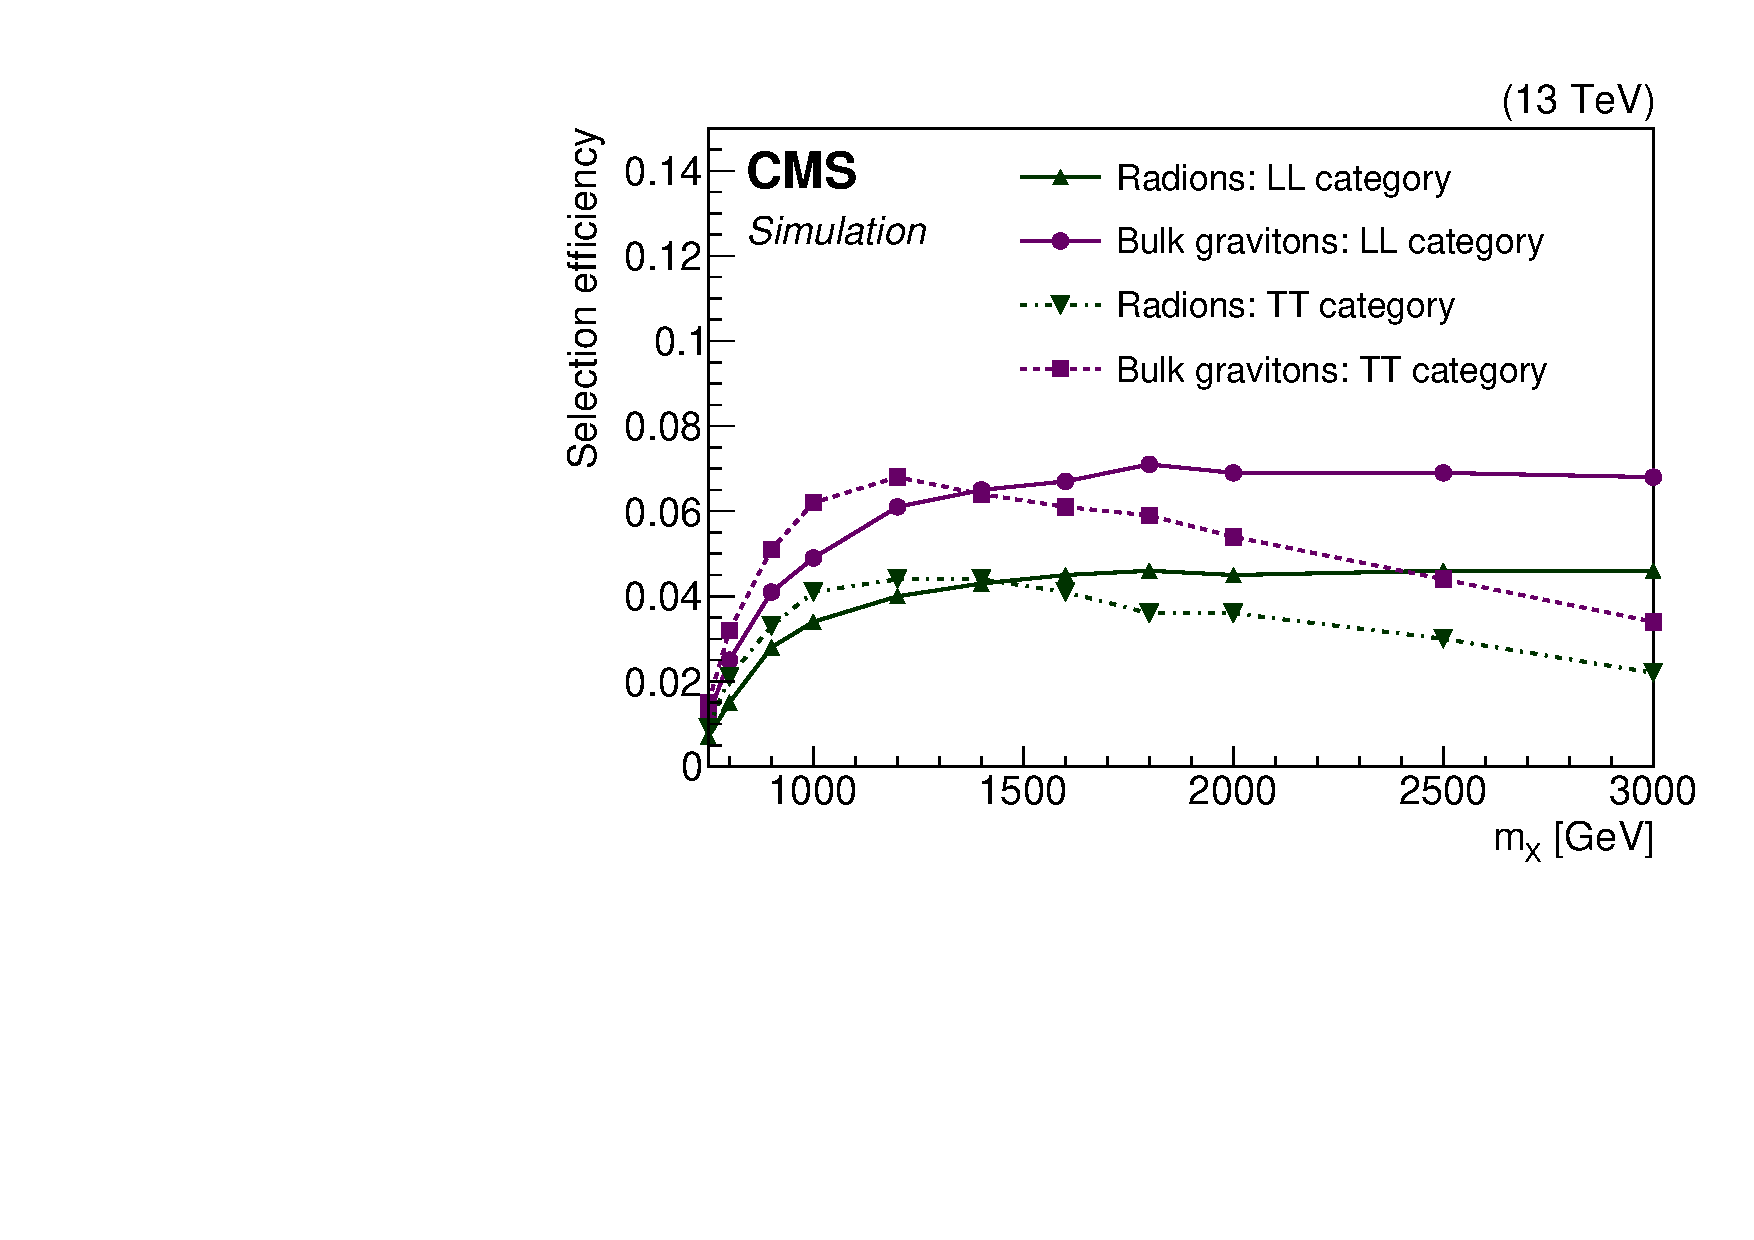
\includegraphics[width=3.5 in]{Analysis/EventSelection/DoubleBSigEff.pdf}
\end{center}
\caption{The signal selection efficiencies for the bulk graviton and radion models for different mass hypotheses of the resonances, shown for the LL and the TT signal event categories. Owing to the large sample size of the simulated events, the statistical uncertainties are negligible.}
\label{fig:DoubleBEff}
\end{figure}

%\begin{figure}[h!]
%\begin{center}
%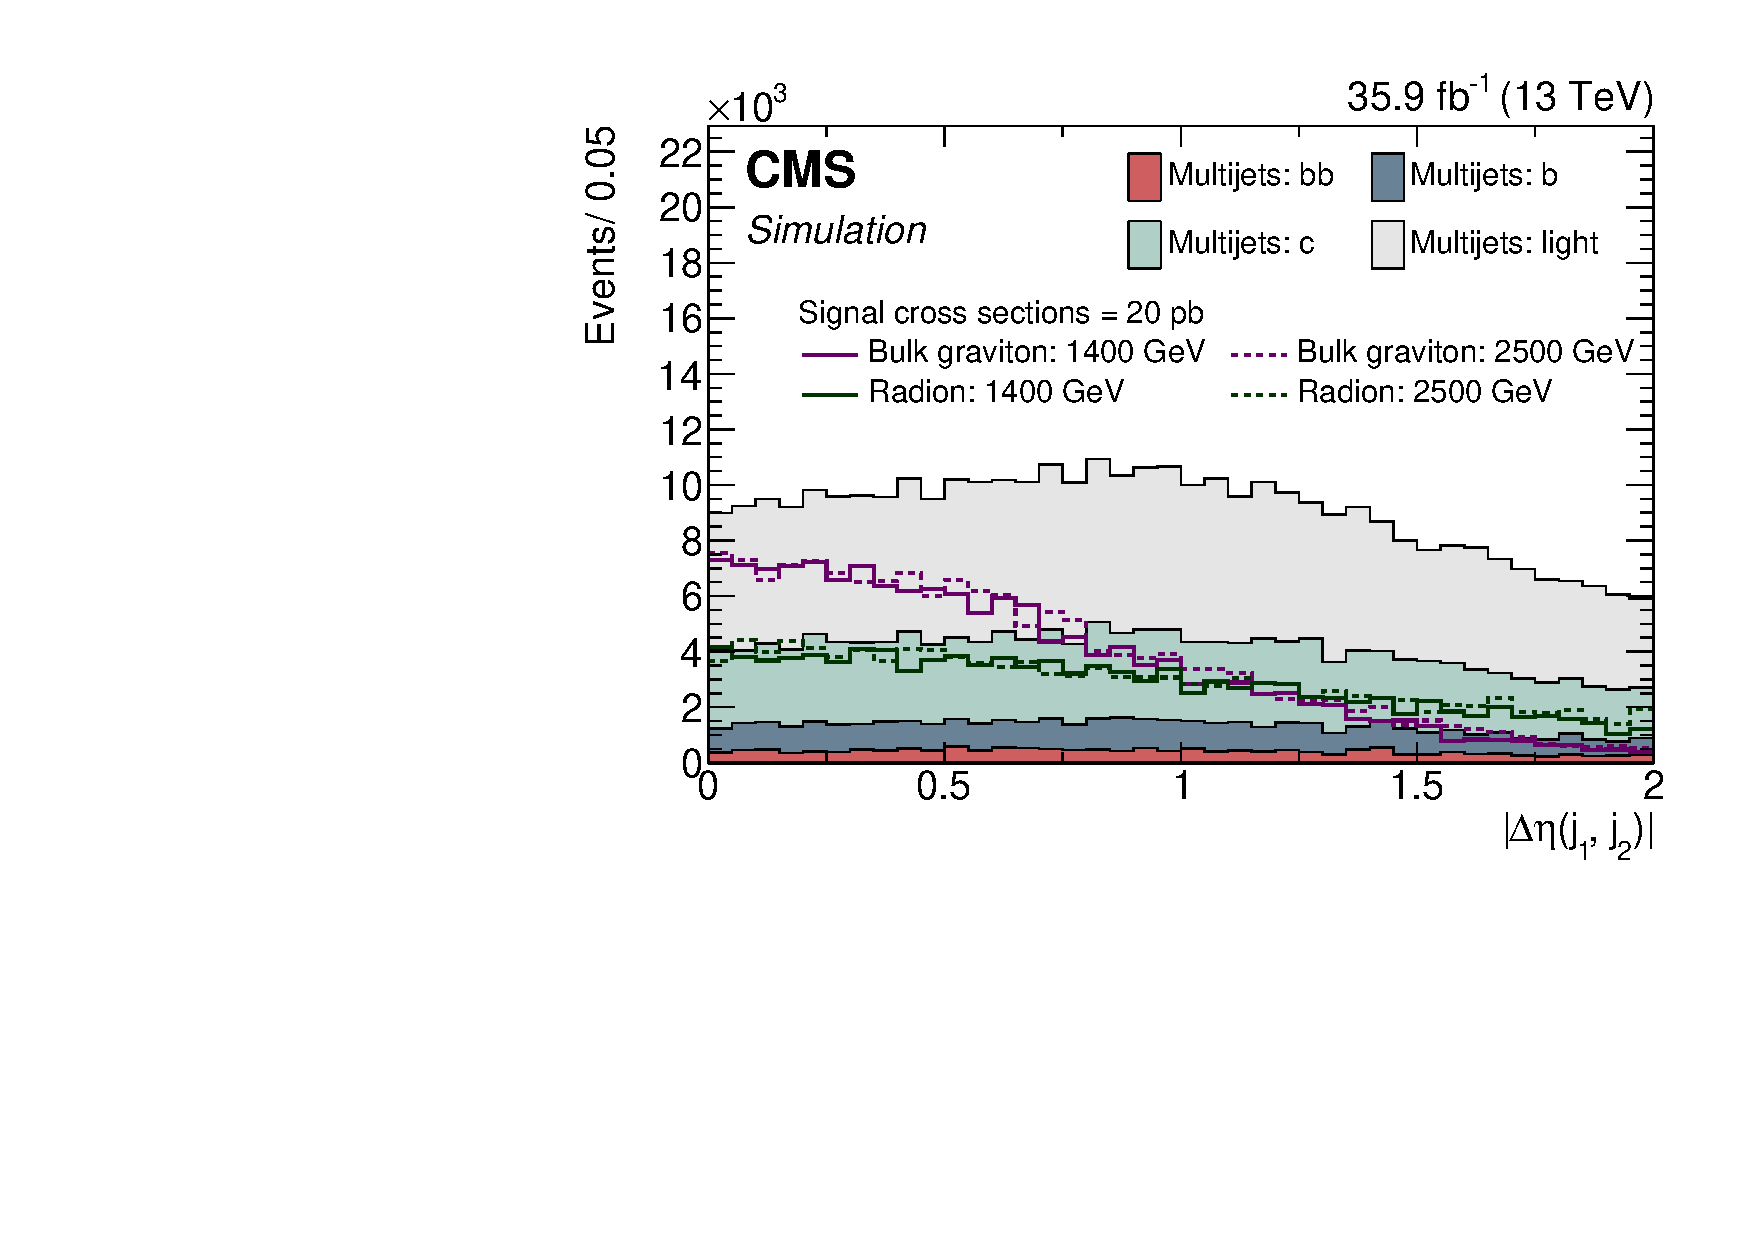
\includegraphics[width=3.5 in]{Analysis/EventSelection/DeltaEta.pdf}
%\end{center}
%\caption{The jet separation, $|\Delta\eta(\mathrm{j}_{1}, \mathrm{j}_{2})|$, distribution for background and signal events. The multijet background components for the differernt jet flavors are shown: events containing at least one jet with two B hadrons (bb) or a single one (b), events containing a jet having a charm hadron (c), and all other events (light). Also plotted are the distributions for the simulated bulk graviton and radion signals of masses 1400 and 2500 GeV assuming a signal cross section of $20$ pb. The numbers of signal and background events correspond to an integrated luminosity of 35.9 $\mathrm{fb}^{-1}$. The full event selection other than $|\Delta\eta(\mathrm{j}_{1}, \mathrm{j}_{2})| < 1.3$ is applied.}
%\label{fig:DeltaEta}
%\end{figure}

\begin{figure}[h!]
\centering
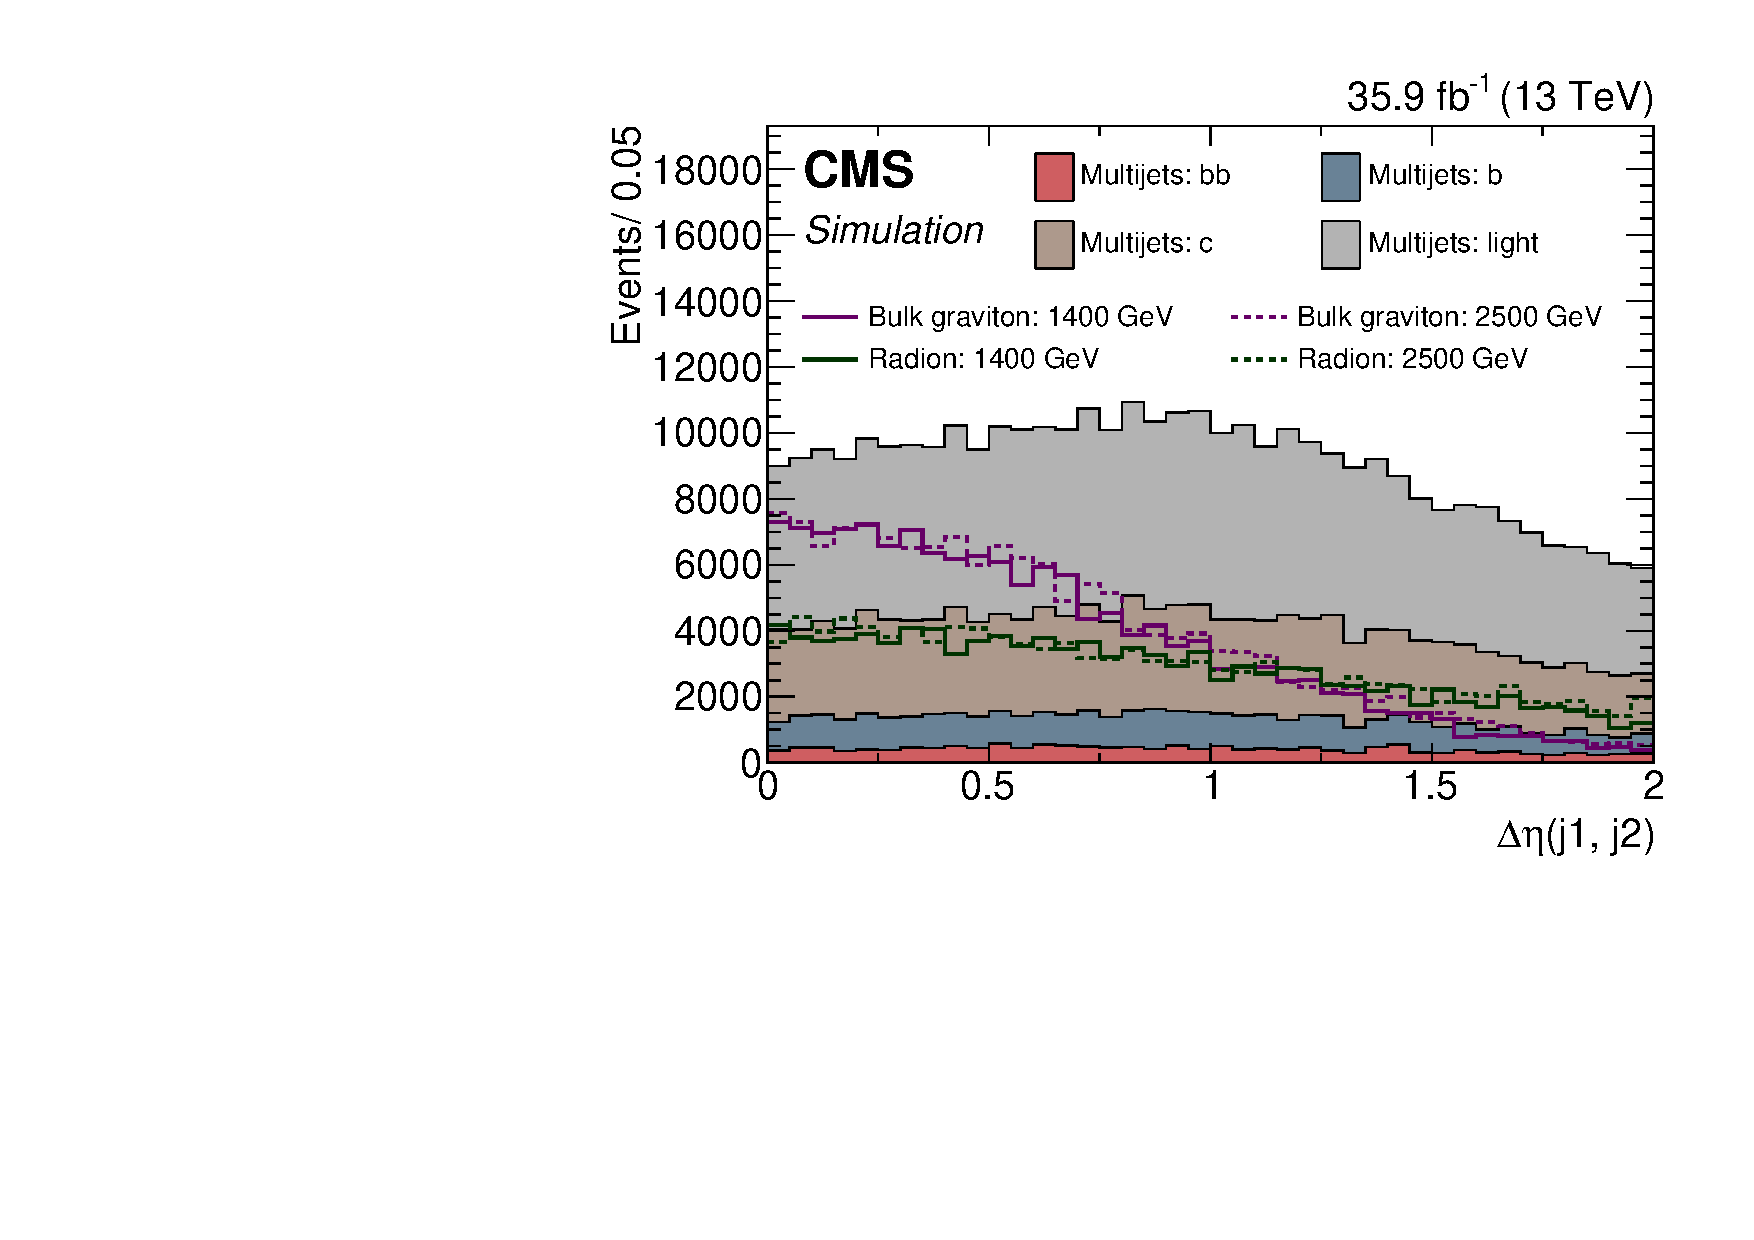
\includegraphics[width=0.45\textwidth]{Analysis/EventSelection/cmc_deltaEta.pdf} \\
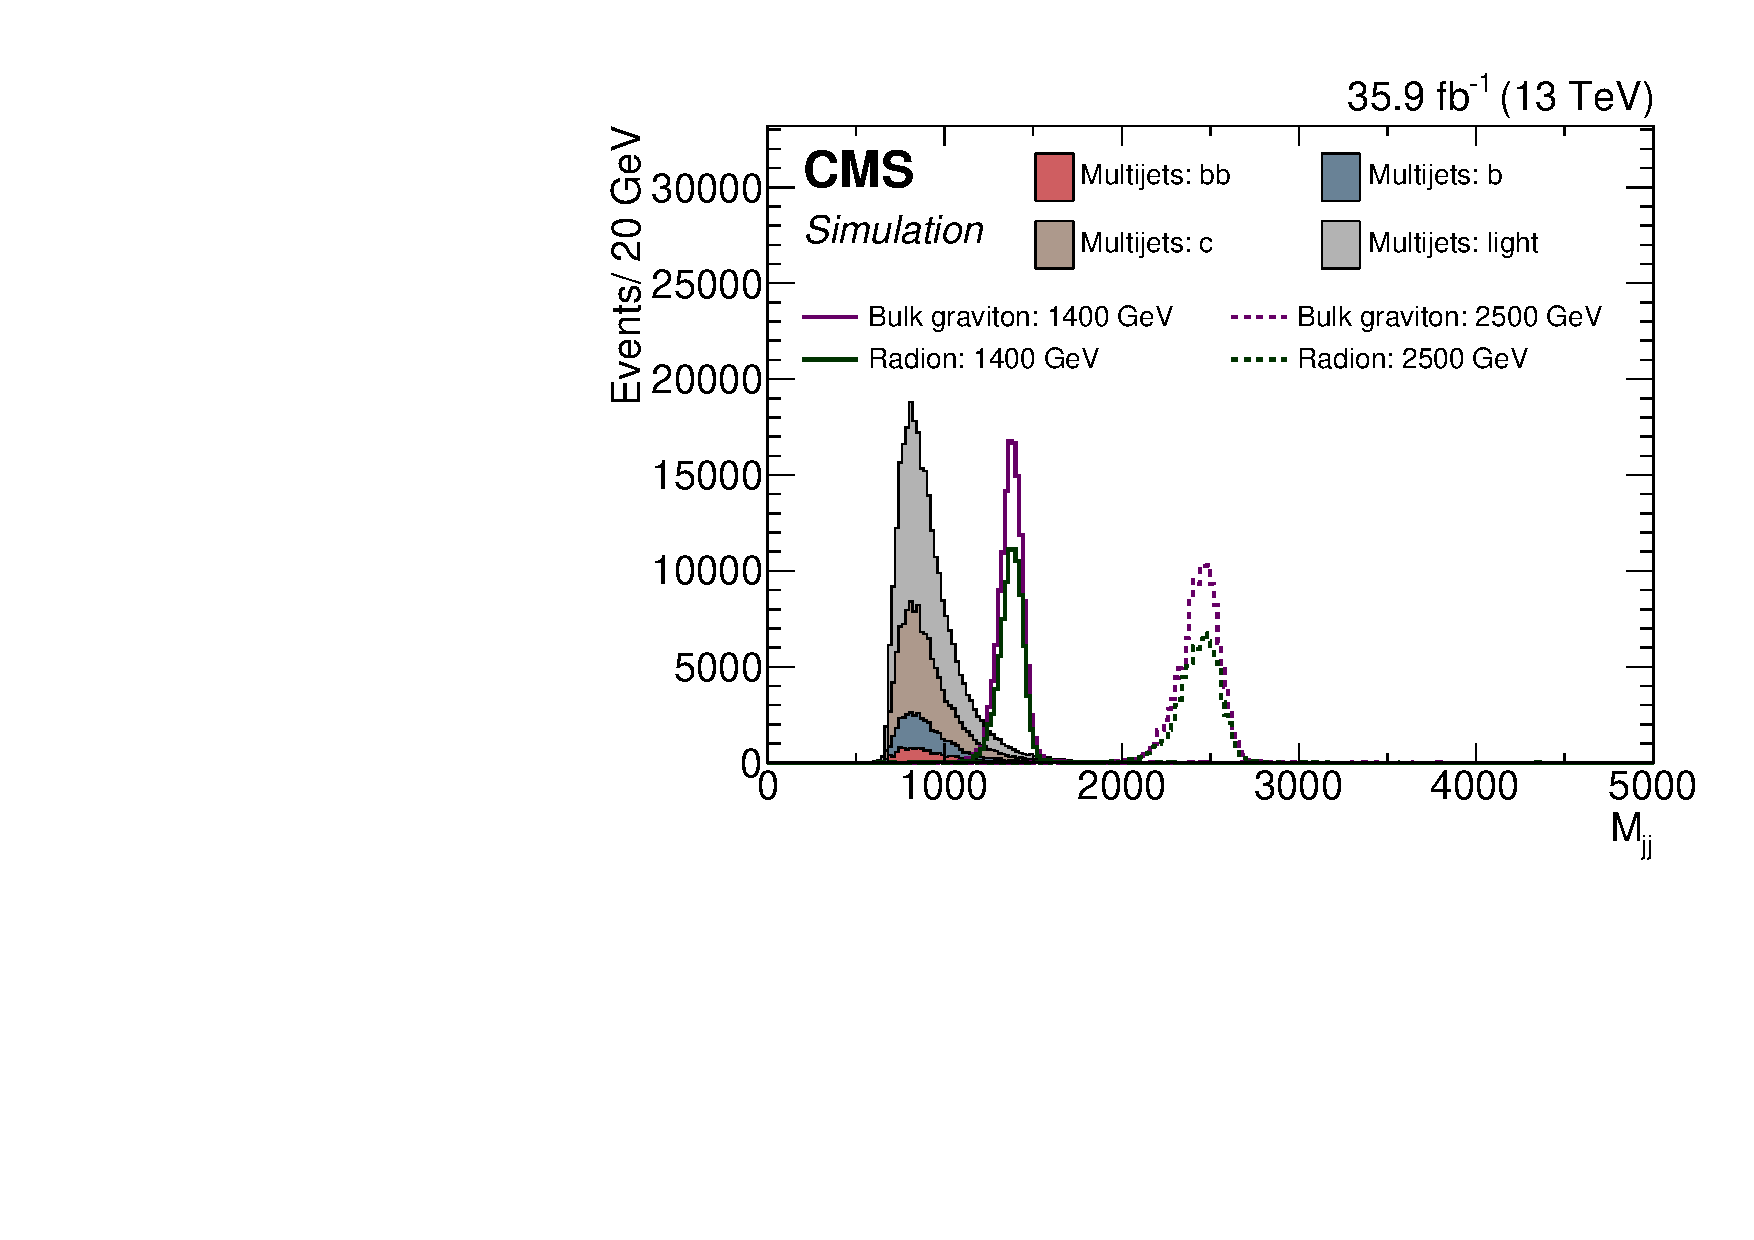
\includegraphics[width=0.45\textwidth]{Analysis/EventSelection/cmc_totalMass.pdf}
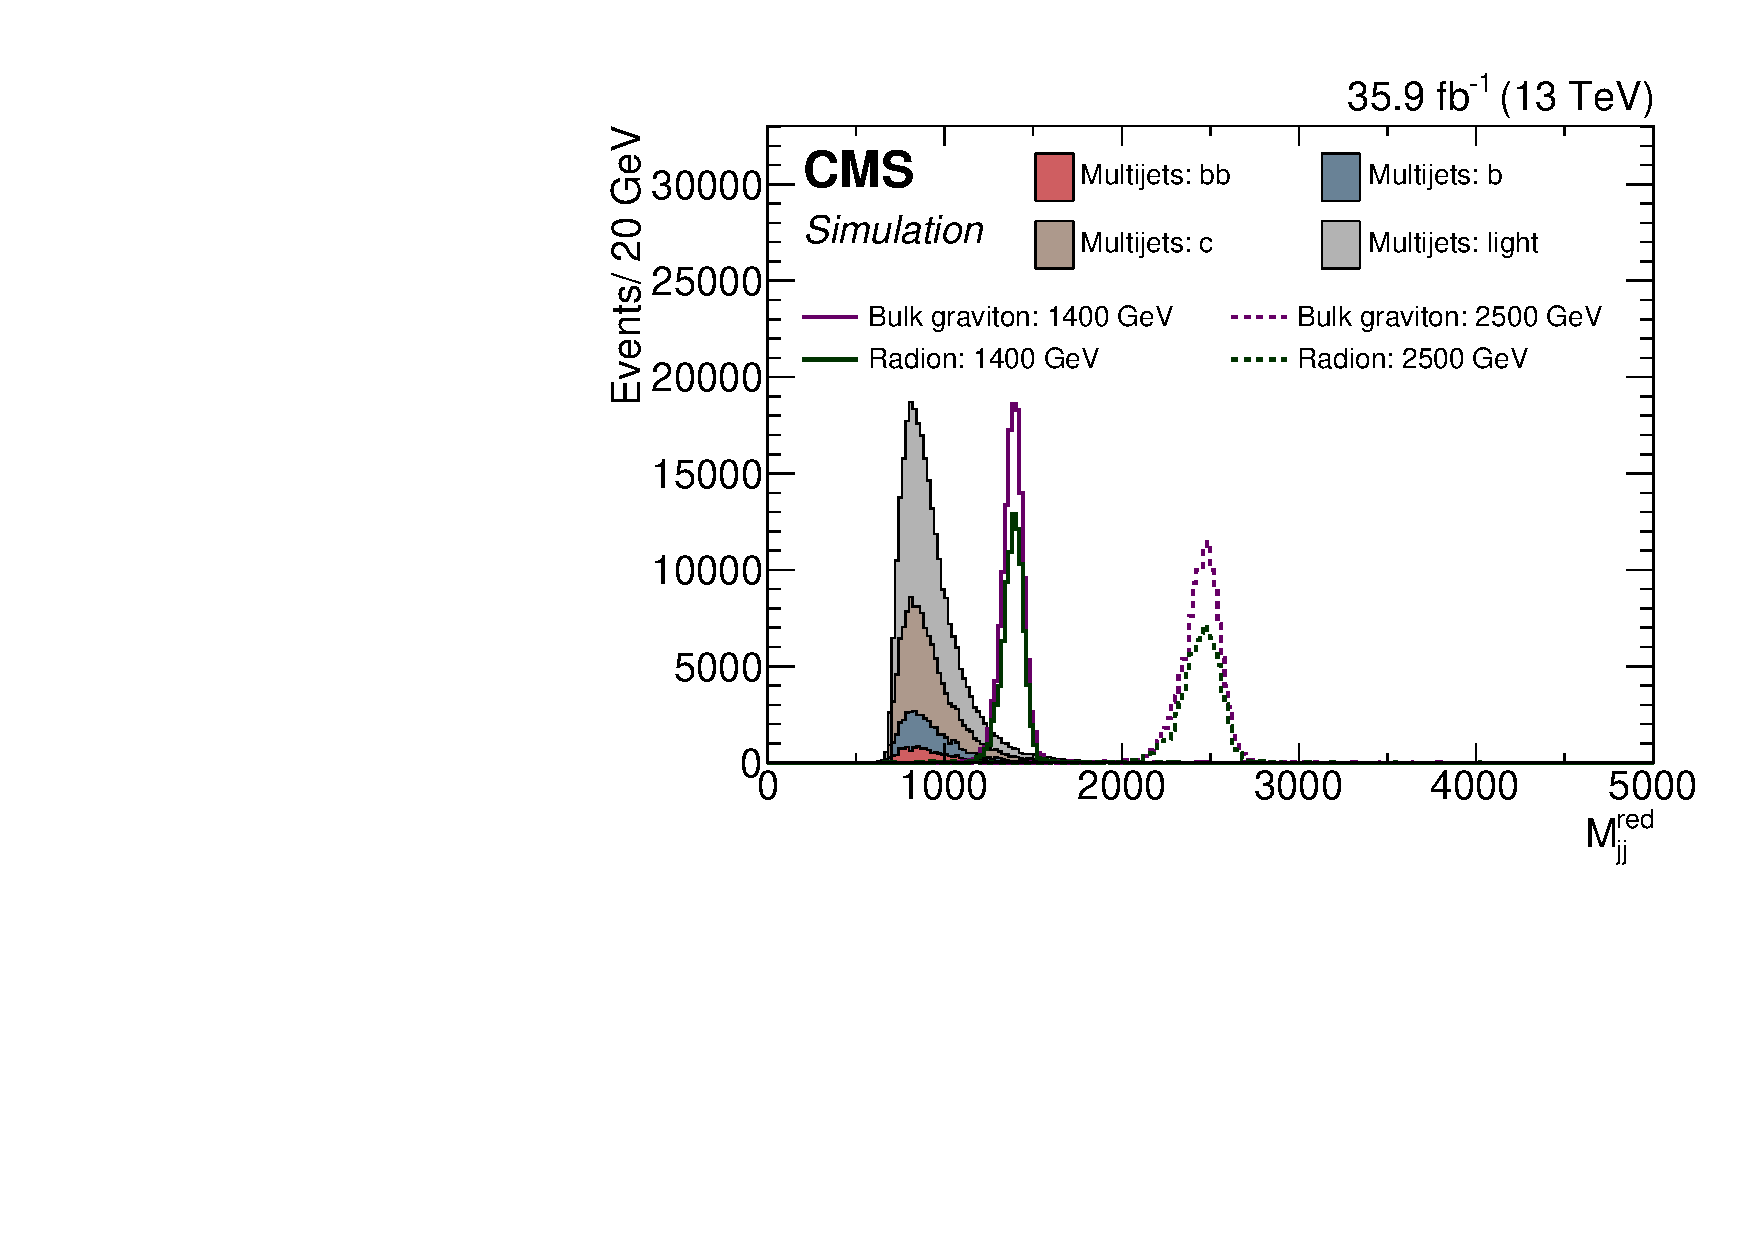
\includegraphics[width=0.45\textwidth]{Analysis/EventSelection/cmc_totalMassRed.pdf}
\caption{ Comparison of simulated events after the full selection excluding b-tagging, $|\Delta\eta(\mathrm{j}_{1}, \mathrm{j}_{2})|$ (upper), $m_{jj}$ (lower left), and $m_{jj}^{red}$ (lower right). A signal cross section of 20~pb is assumed for each signal mass point.
\label{fig:eventToplogy_prebtag}
}
\end{figure}

\begin{figure}[h!]
\centering
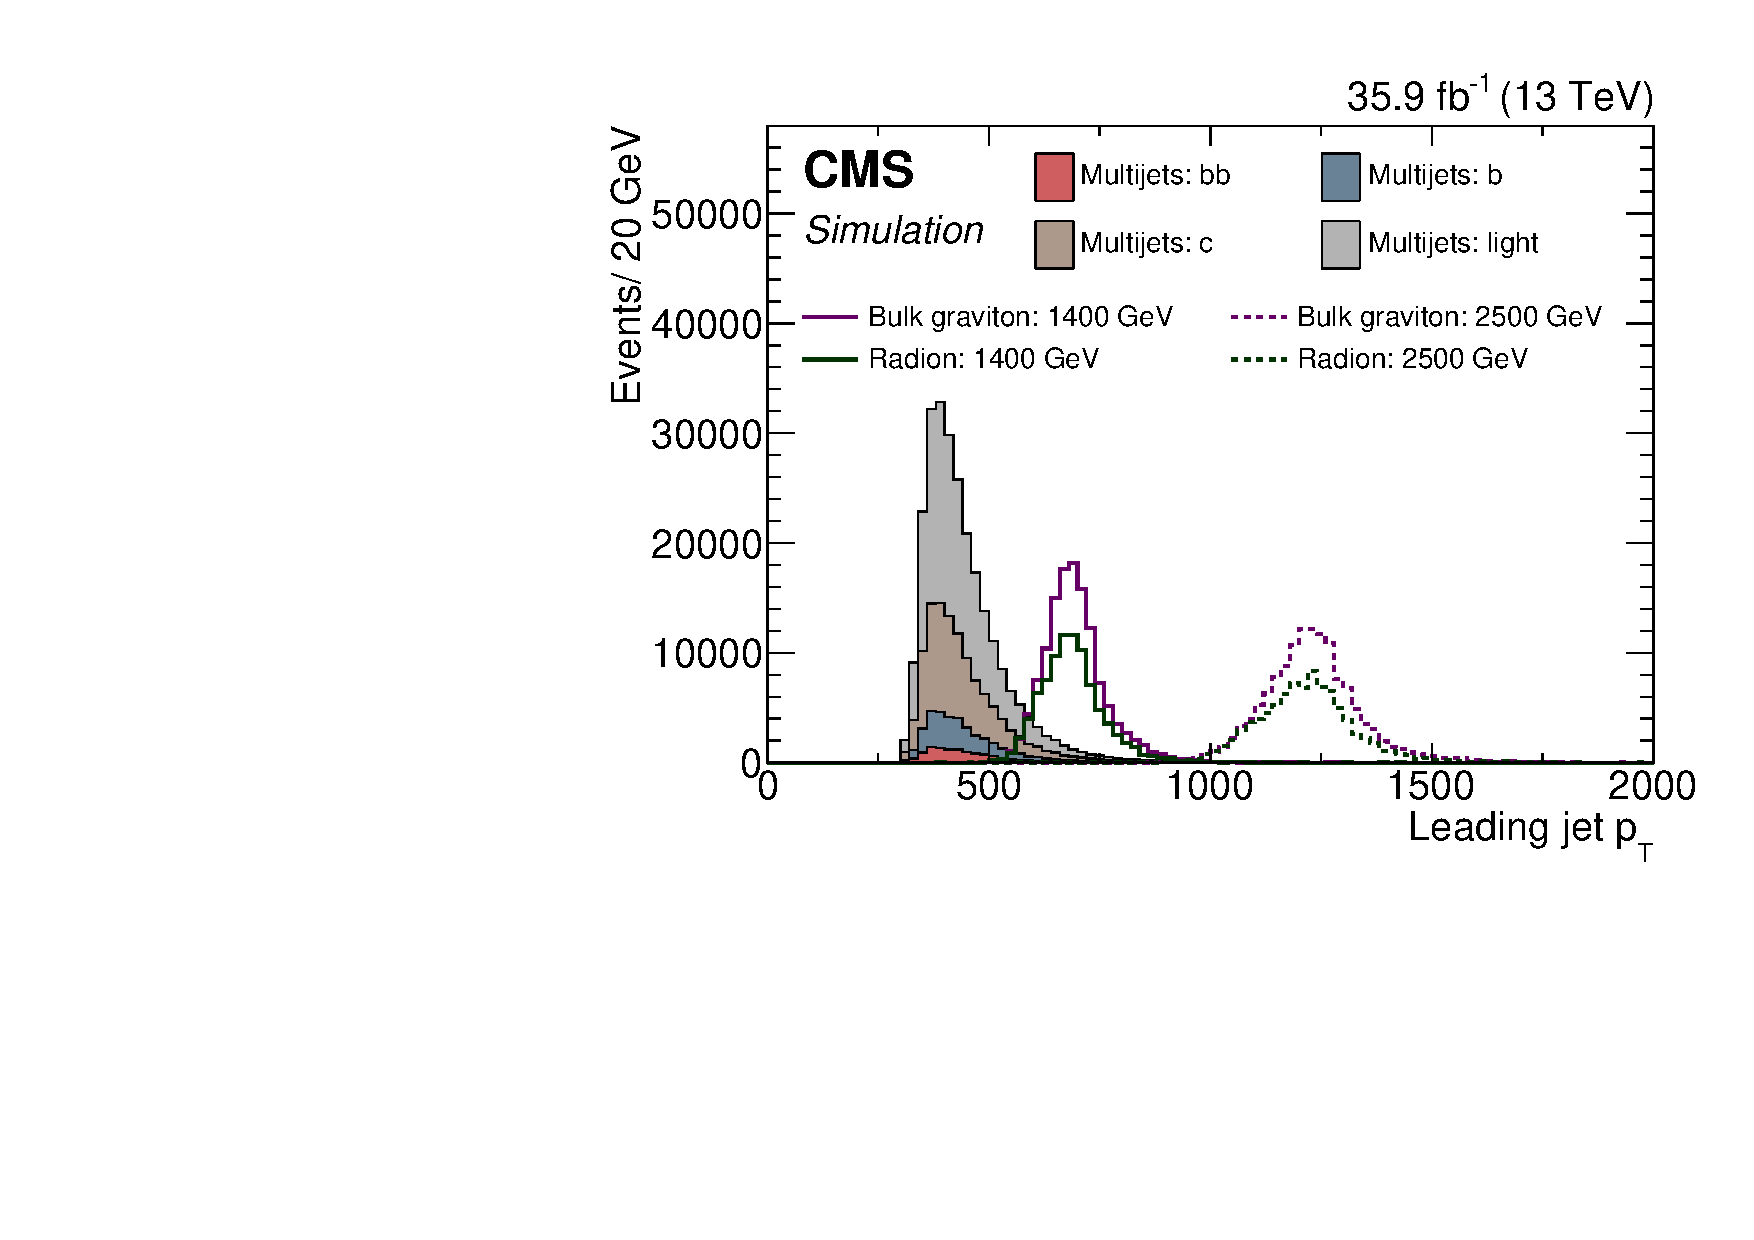
\includegraphics[width=0.45\textwidth]{Analysis/EventSelection/cmc_pt_j0.pdf}
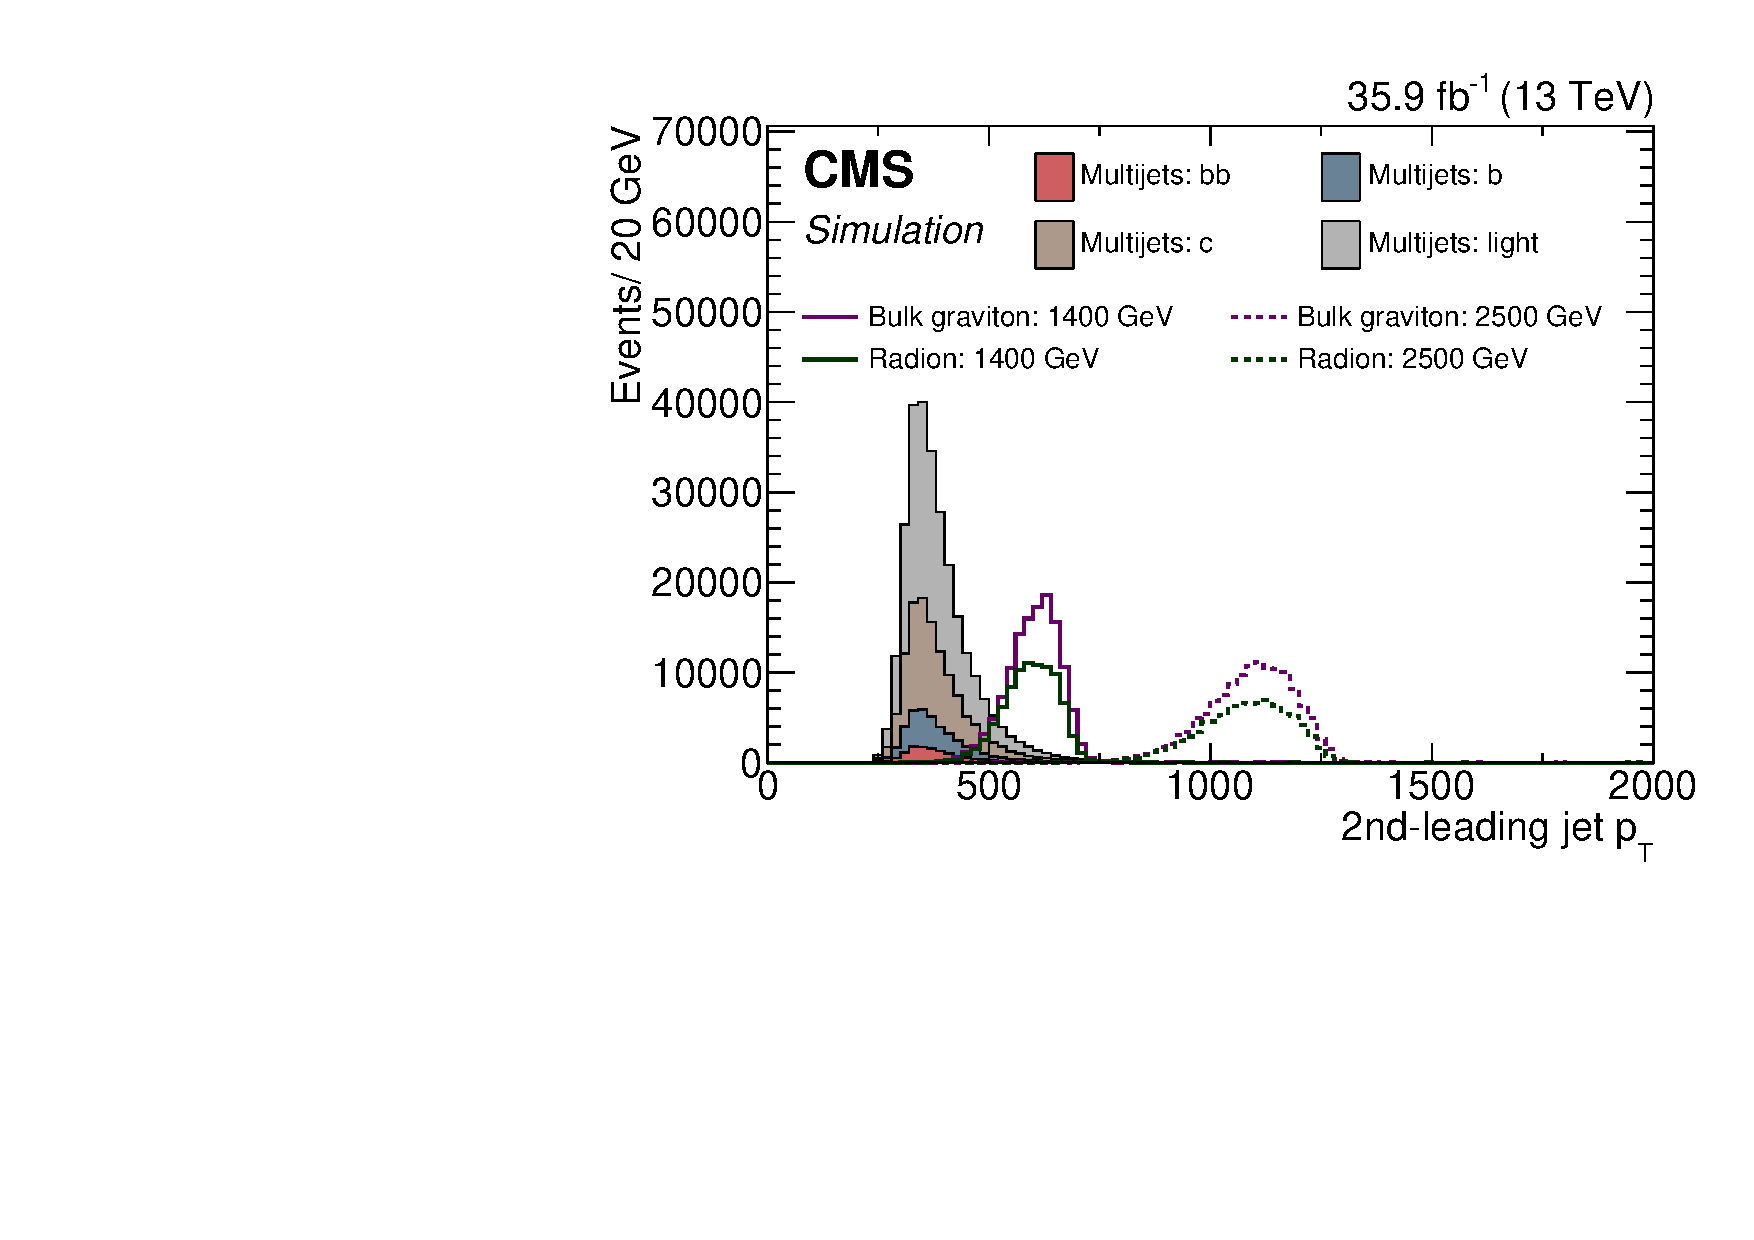
\includegraphics[width=0.45\textwidth]{Analysis/EventSelection/cmc_pt_j1.pdf} \\
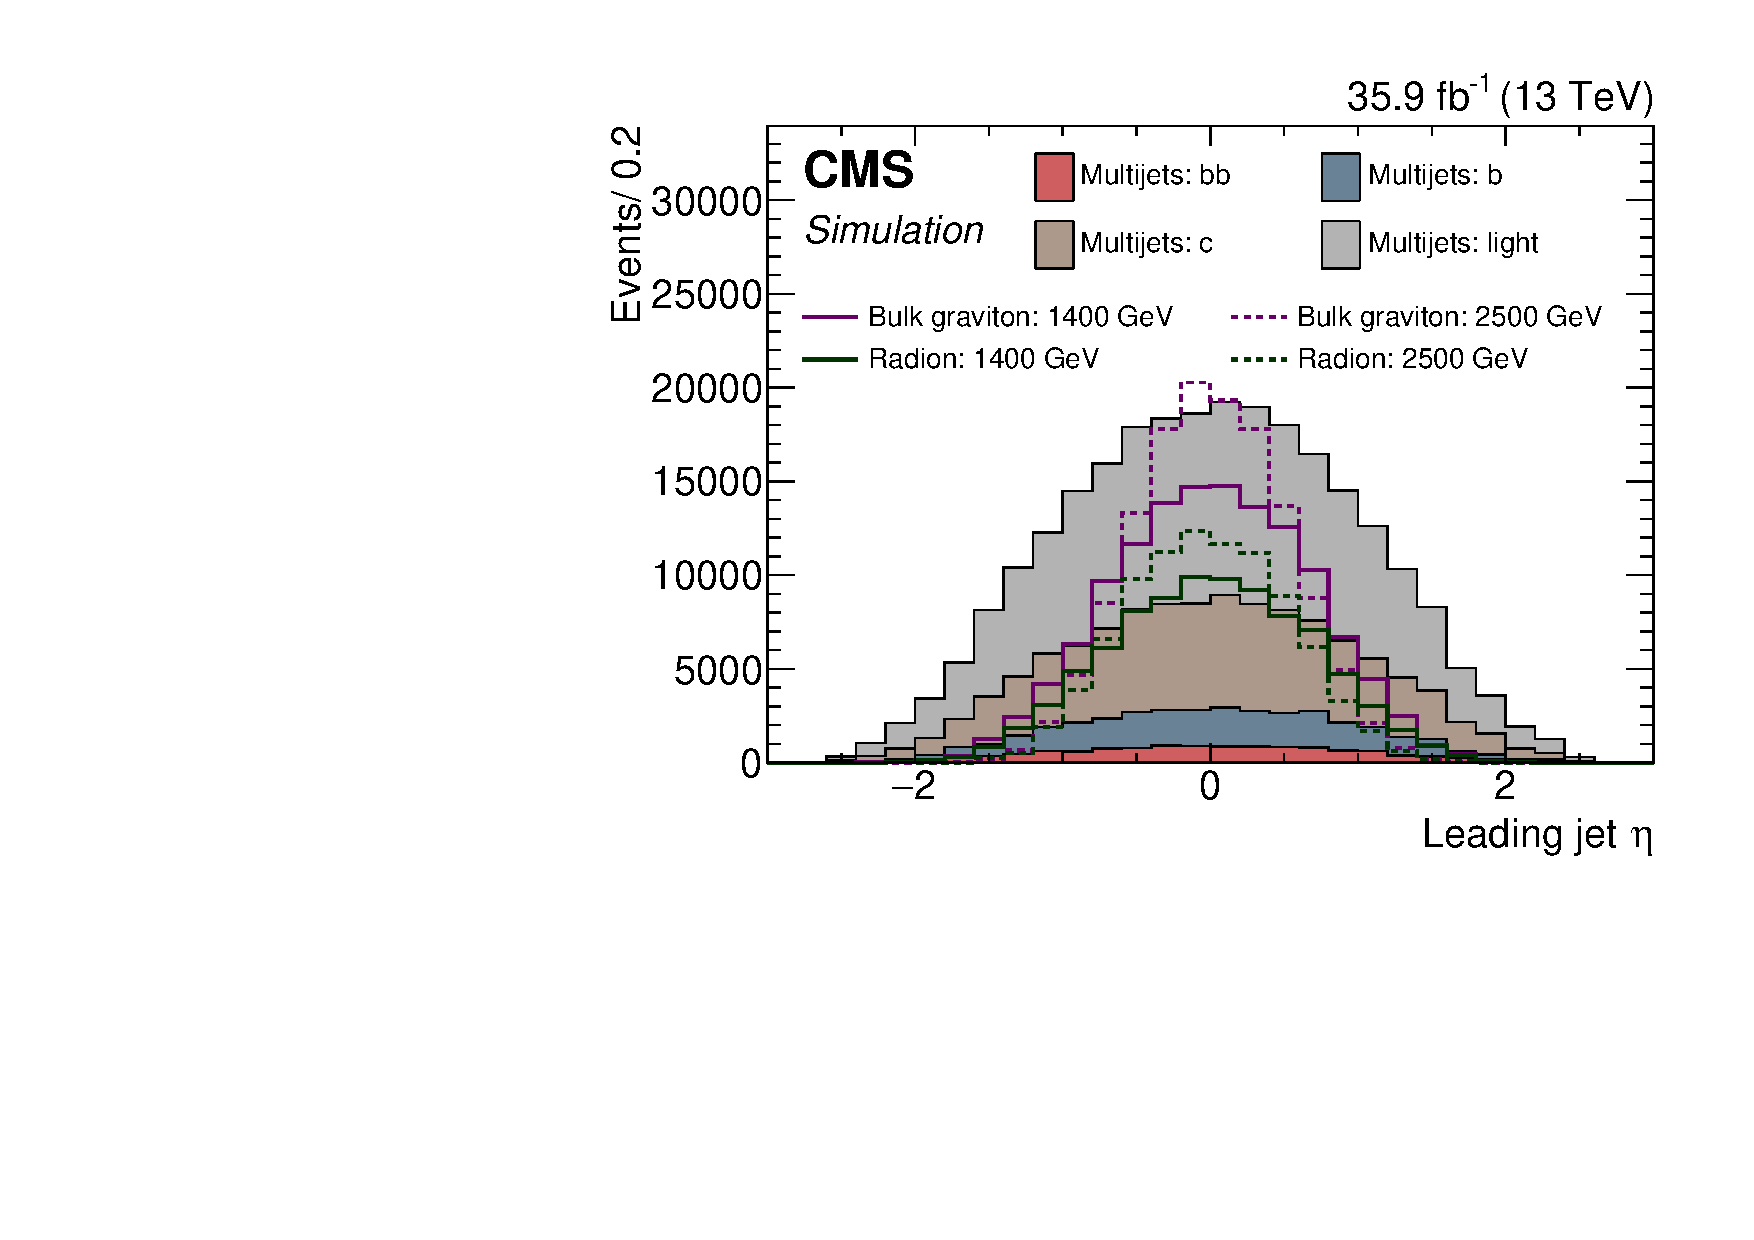
\includegraphics[width=0.45\textwidth]{Analysis/EventSelection/cmc_eta_j0.pdf}
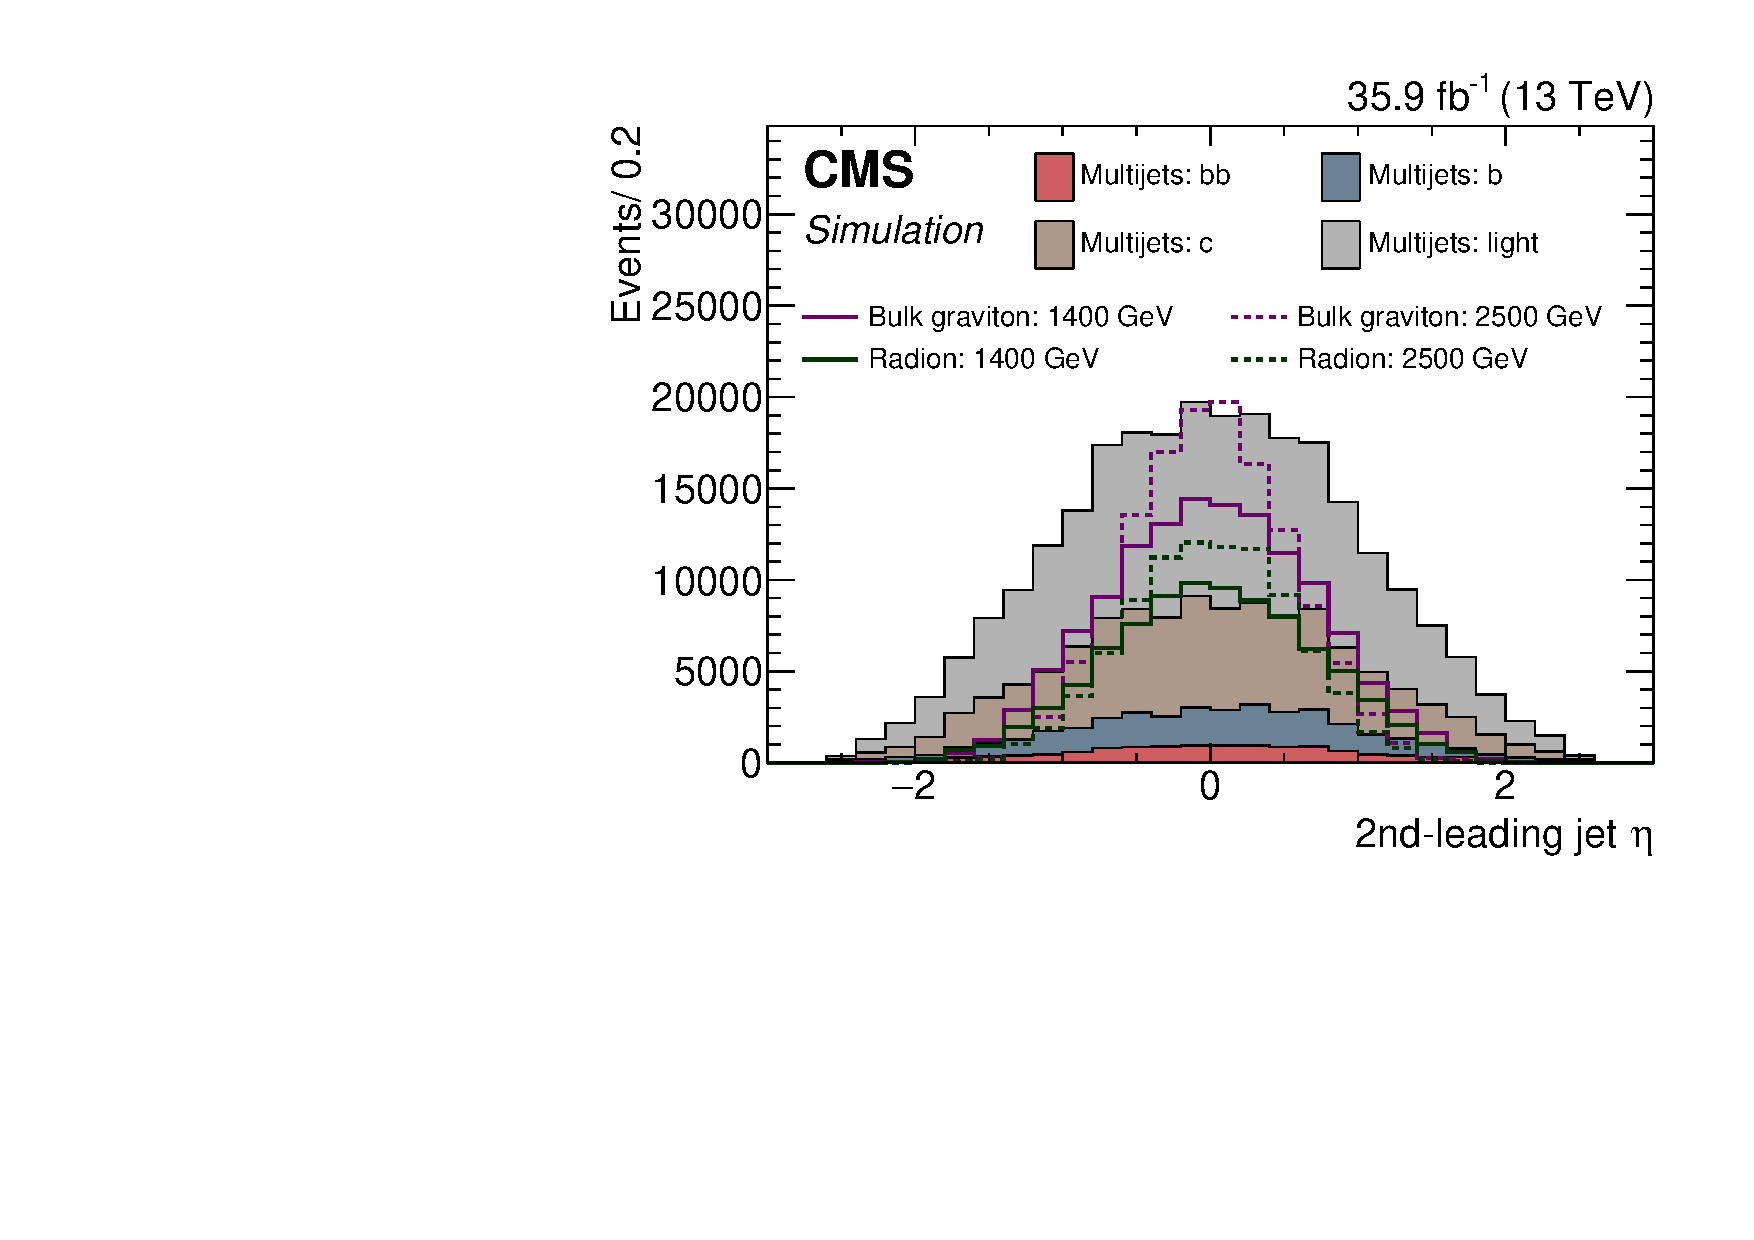
\includegraphics[width=0.45\textwidth]{Analysis/EventSelection/cmc_eta_j1.pdf}
\caption{ Comparison of simulated events after the full selection excluding b-tagging, for the $p_{T}$ (upper) and $\eta$ (lower) of  leading (left) and sub-leading (right) Higgs jets. A signal cross section of 20~pb is assumed for each signal mass point. \label{fig:higgsjet_prebtag}
}

\end{figure}
\begin{figure}[h!]
\centering
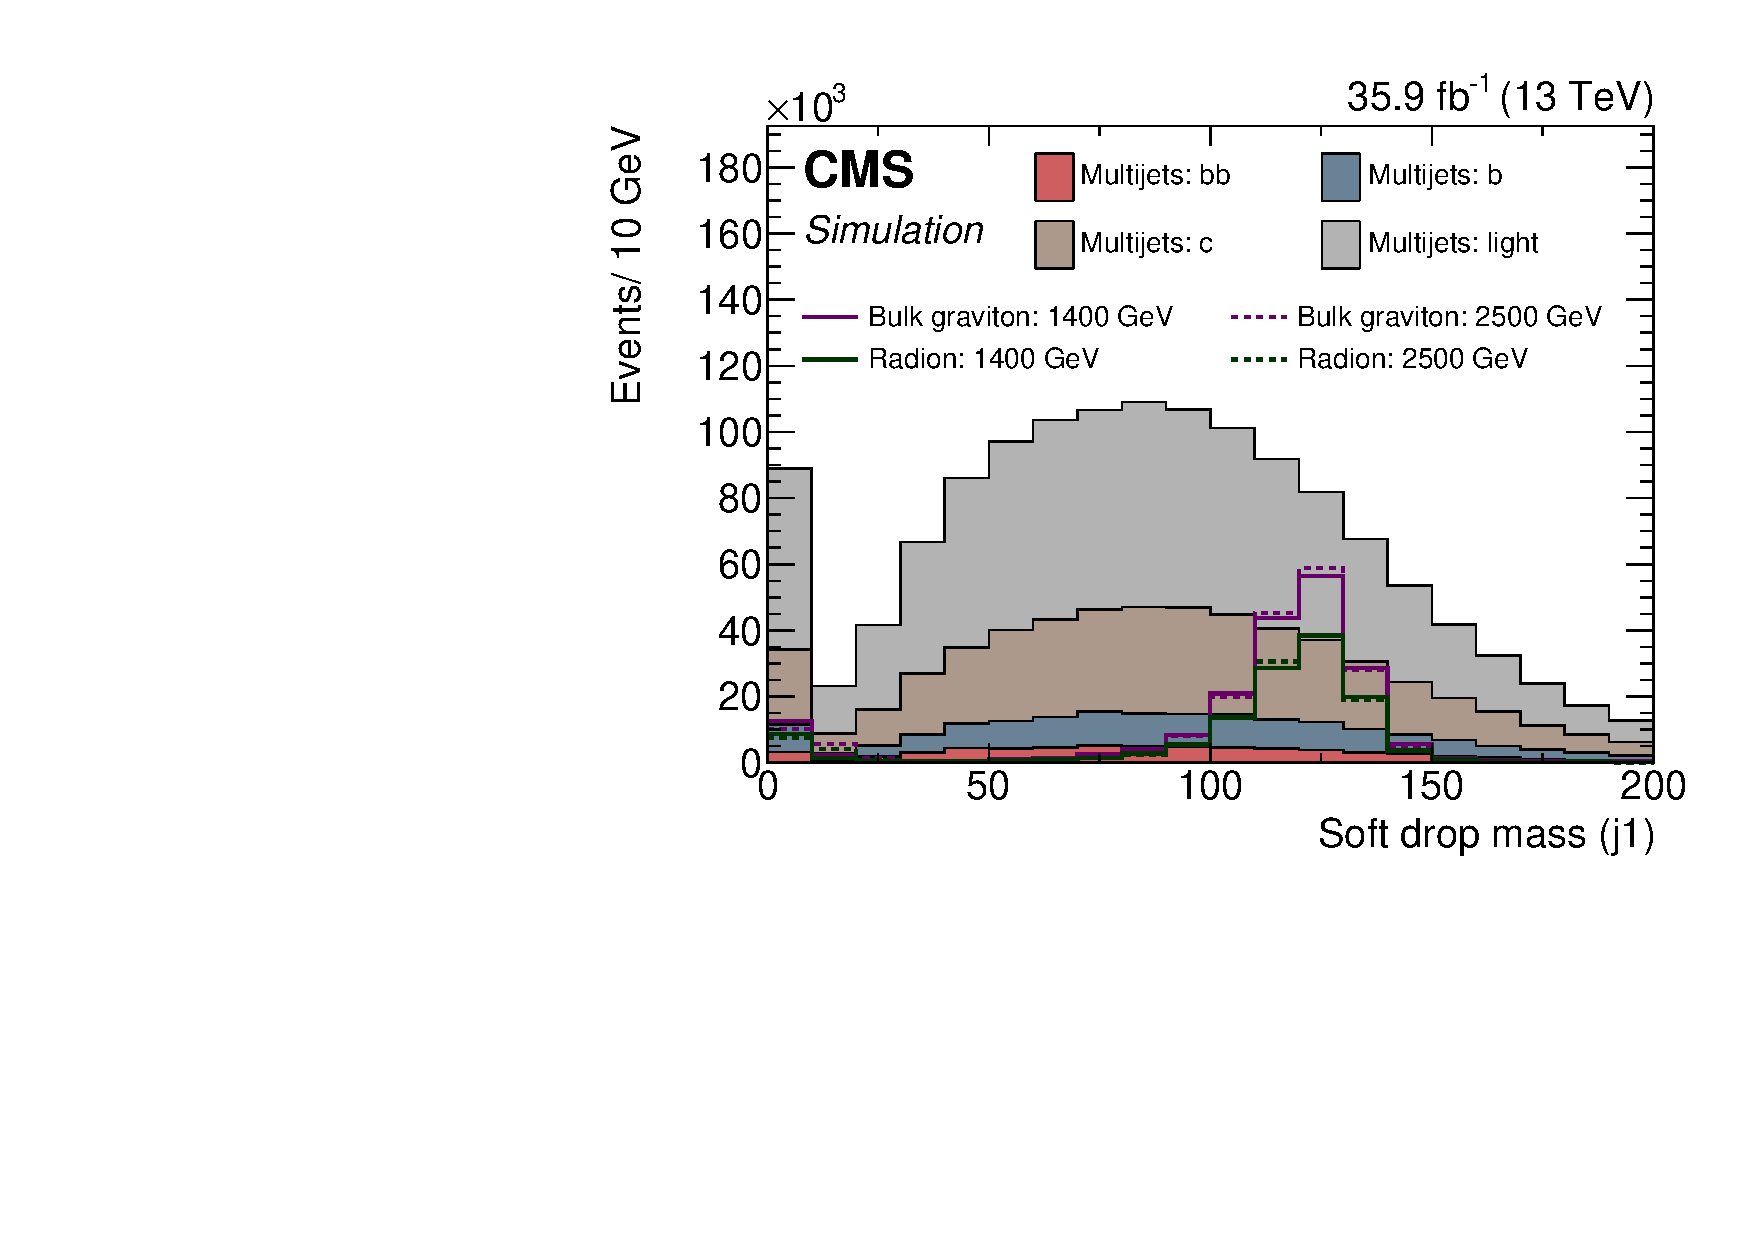
\includegraphics[width=0.45\textwidth]{Analysis/EventSelection/cmc_puppiSDMassThea_j0.pdf}
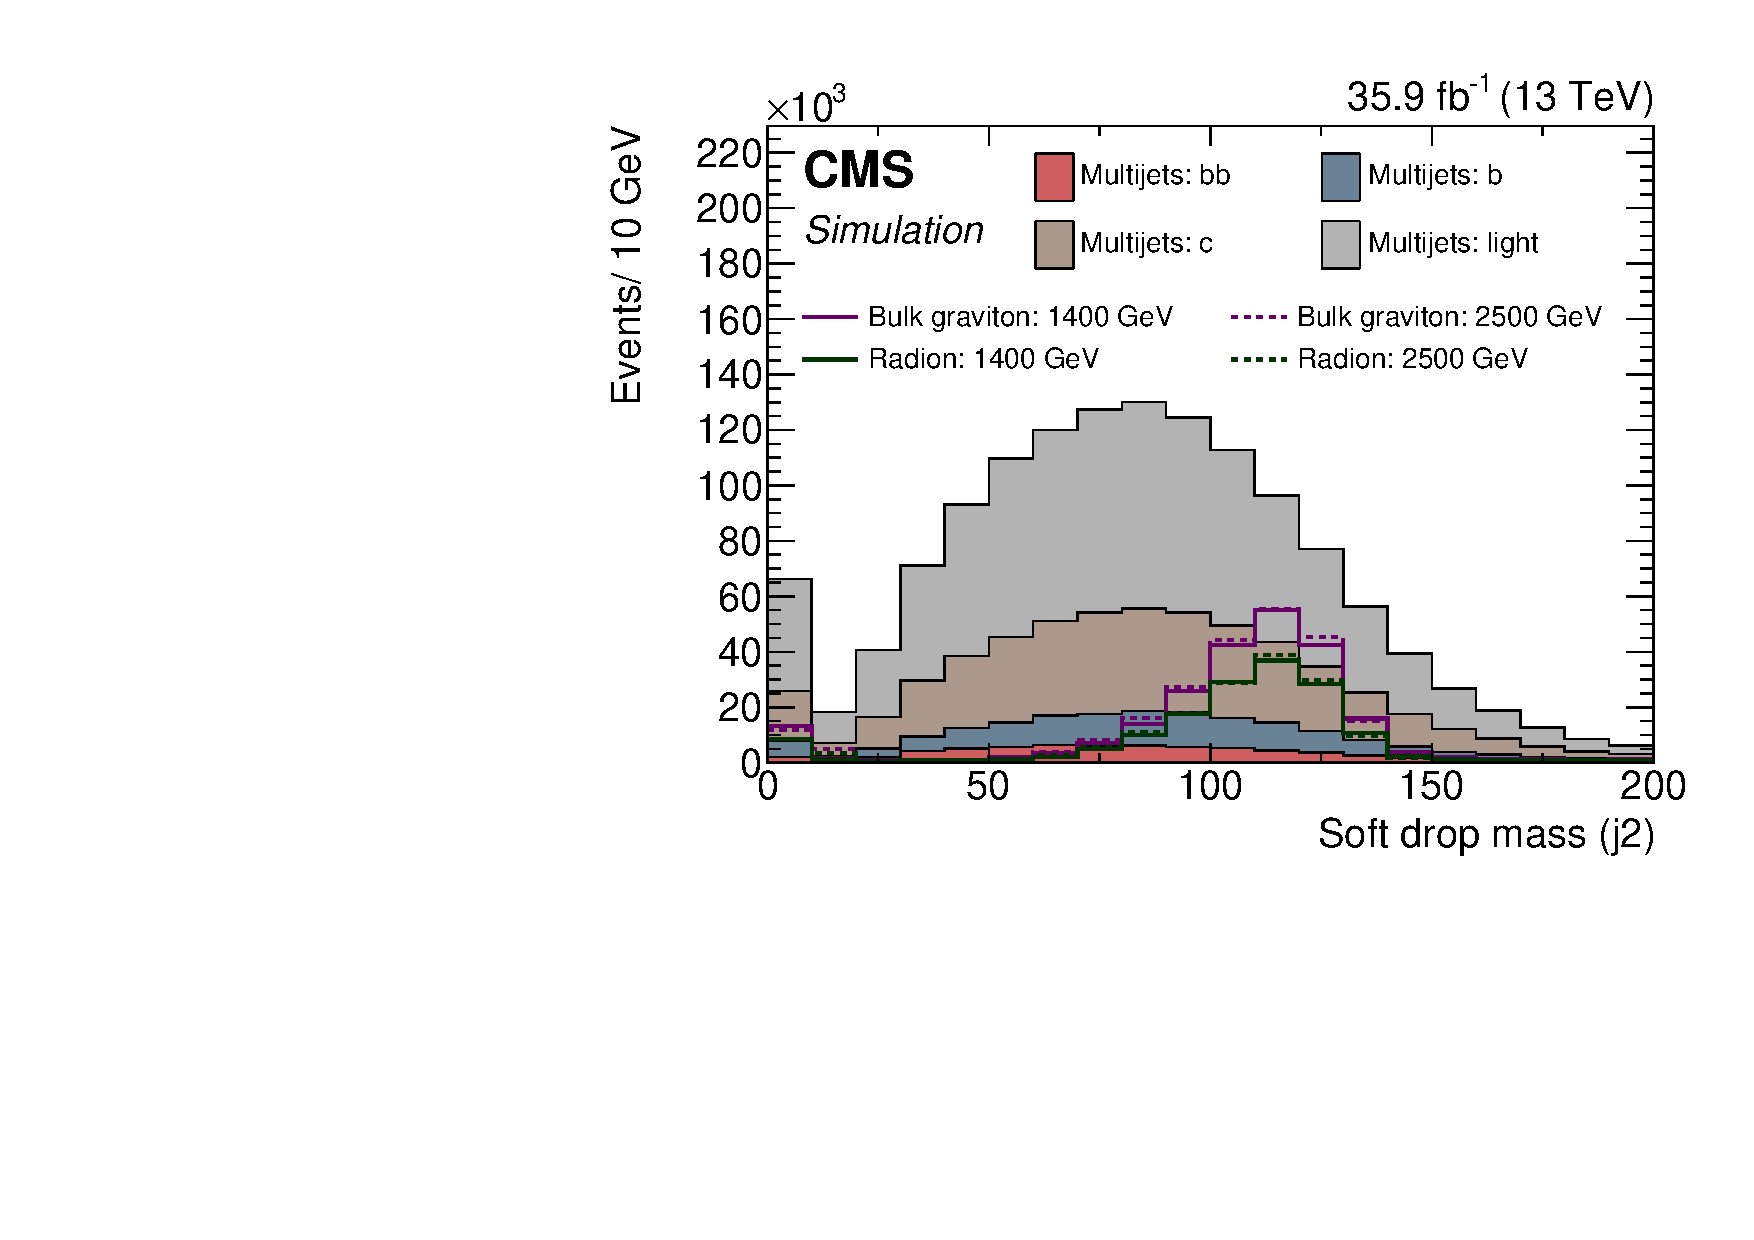
\includegraphics[width=0.45\textwidth]{Analysis/EventSelection/cmc_puppiSDMassThea_j1.pdf} \\
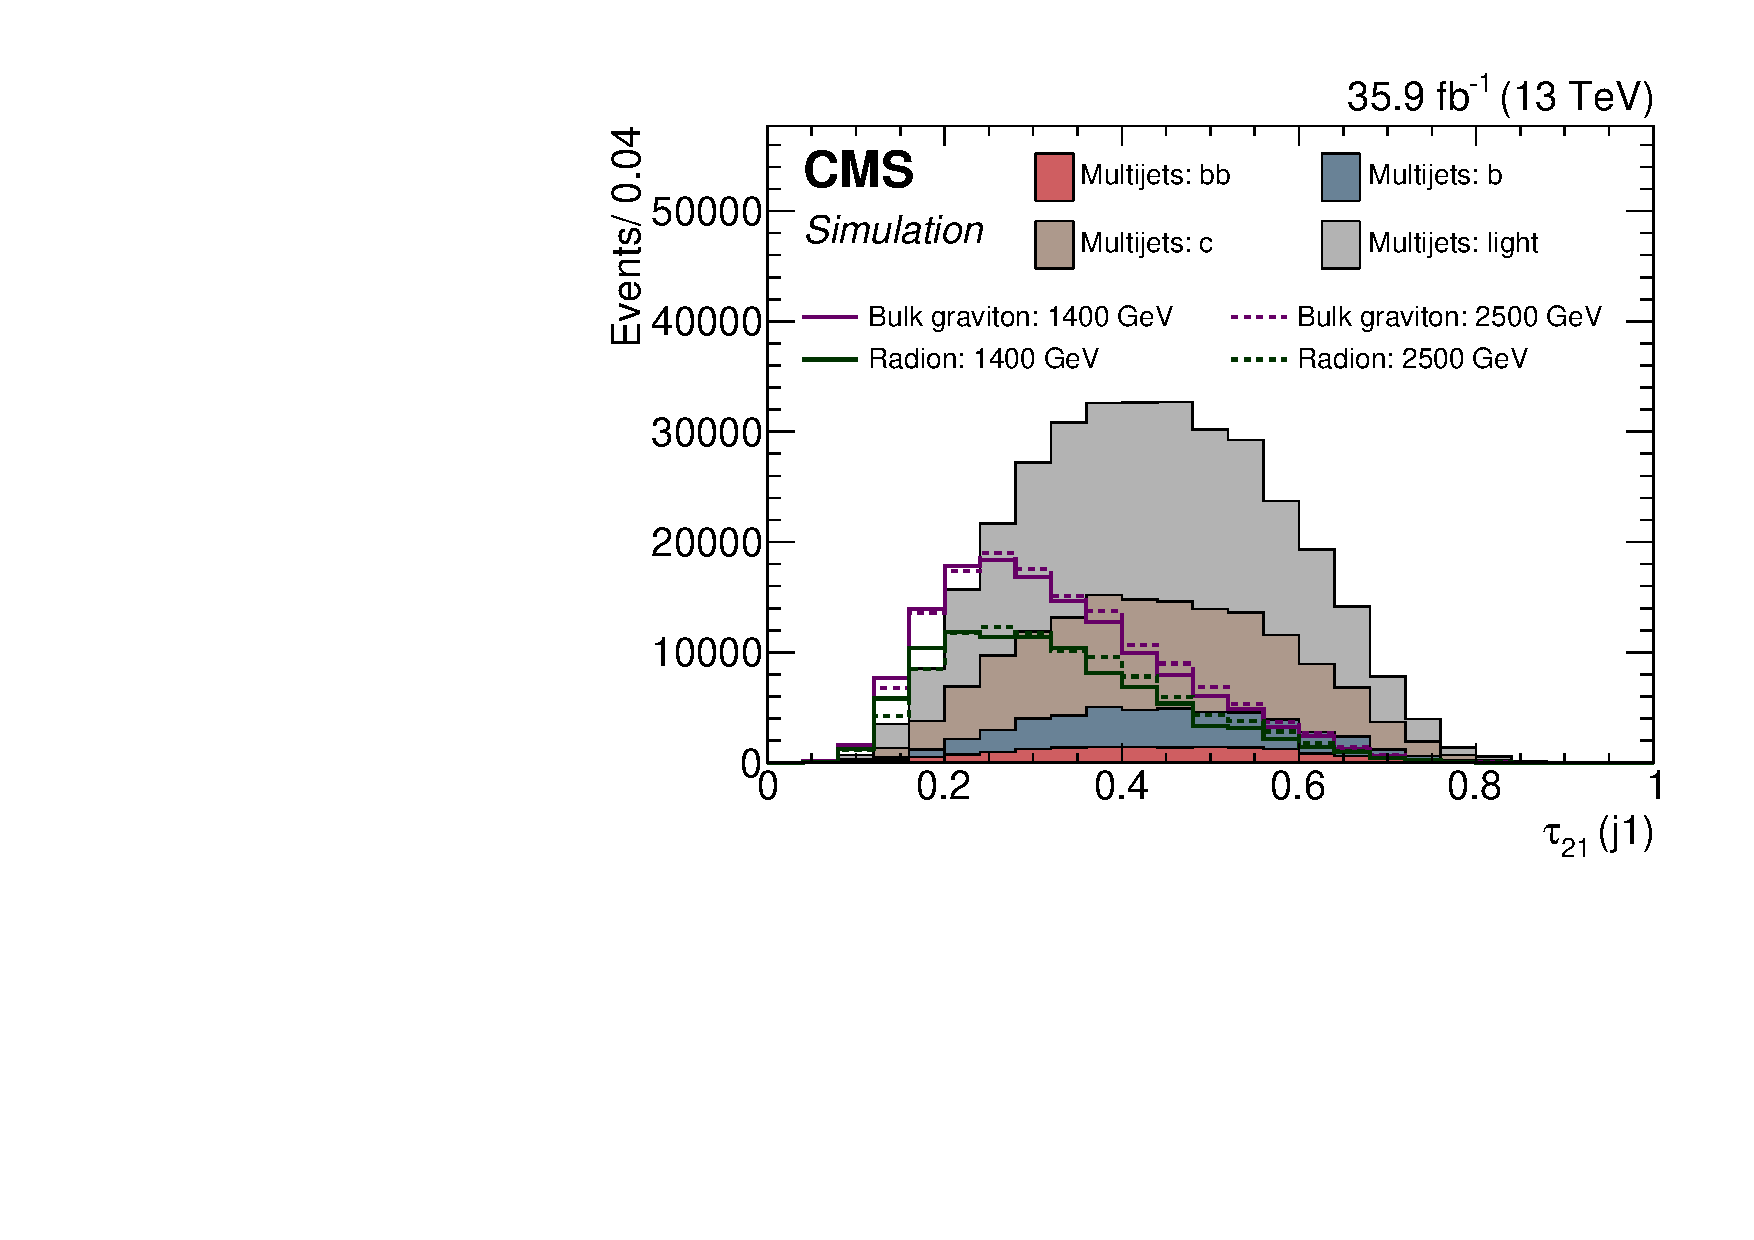
\includegraphics[width=0.45\textwidth]{Analysis/EventSelection/cmc_puppiTau21_j0.pdf}
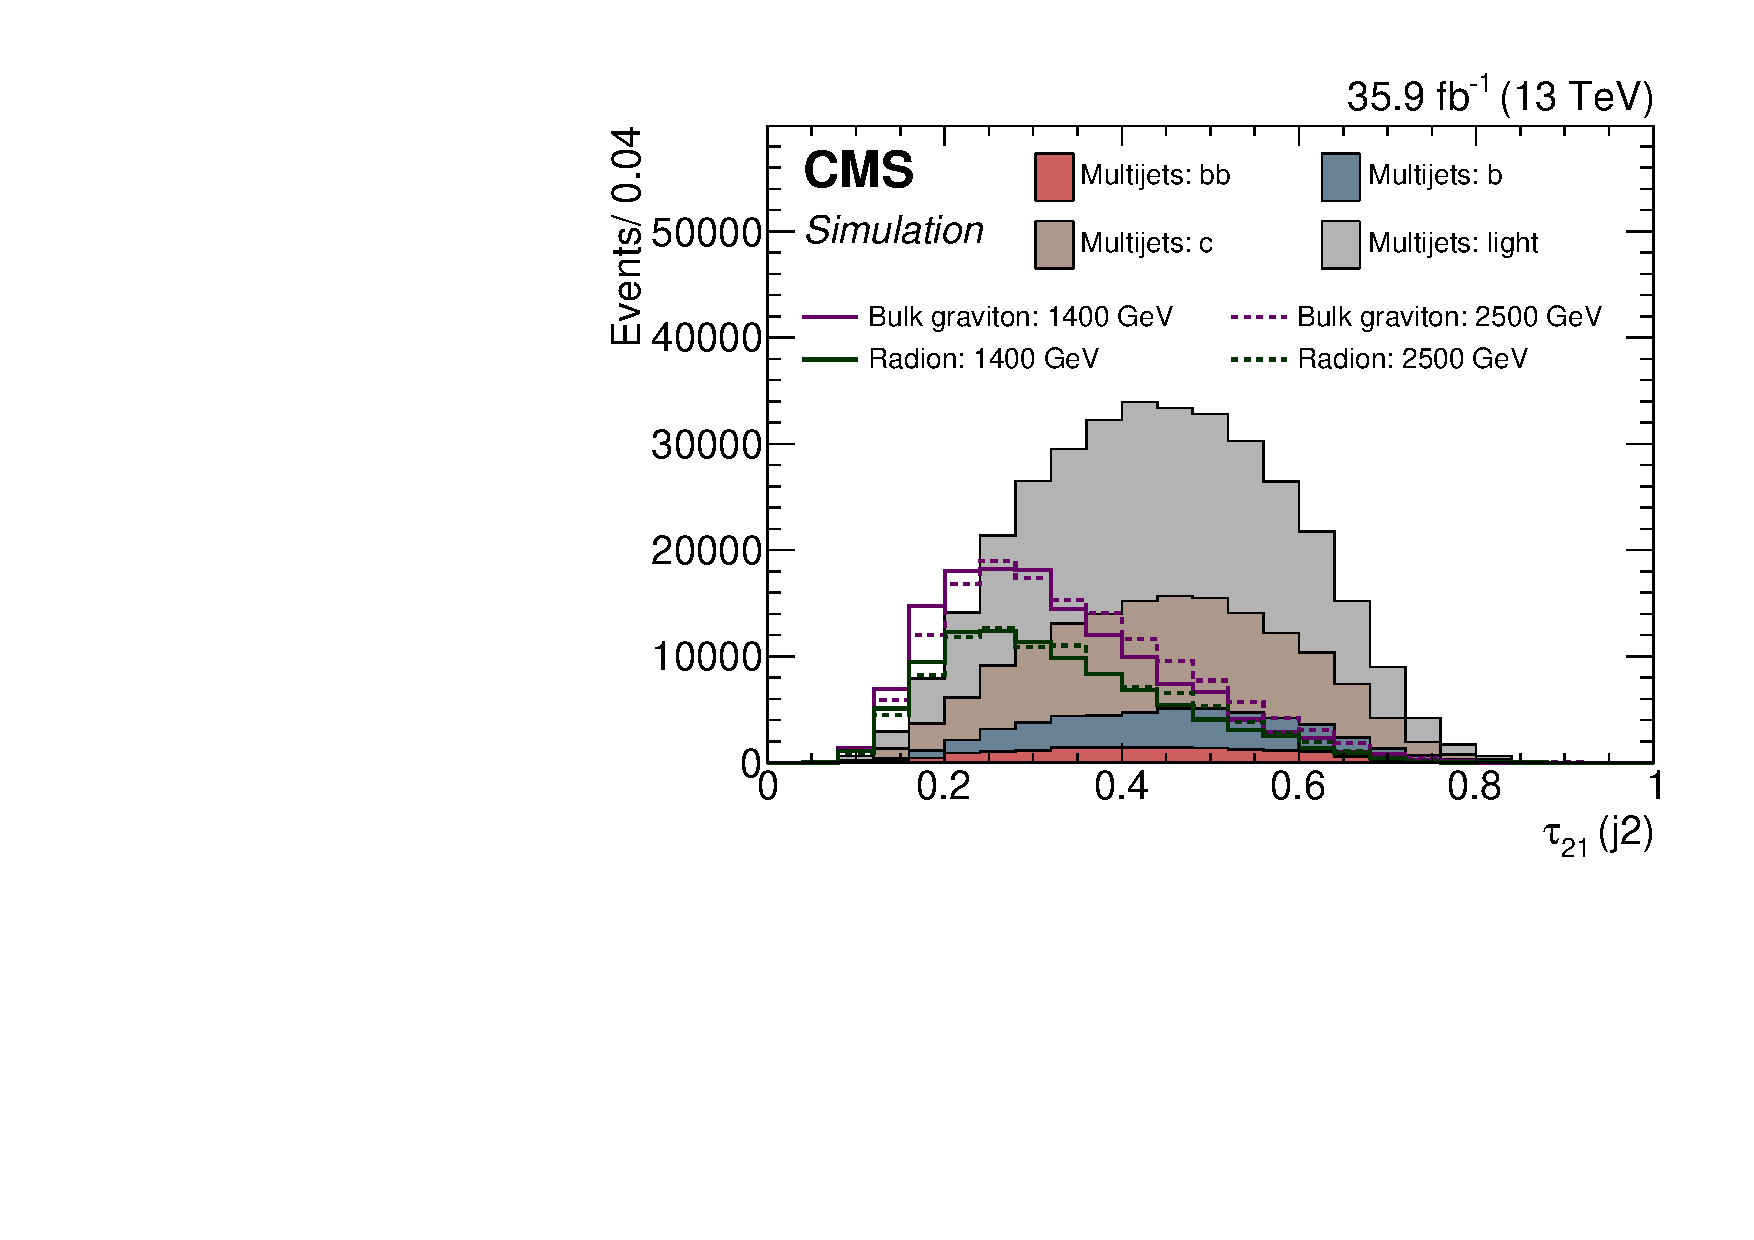
\includegraphics[width=0.45\textwidth]{Analysis/EventSelection/cmc_puppiTau21_j1.pdf}
\caption{ Comparison of simulated events after the full selection excluding b-tagging, for the soft-drop mass (upper)  and the $\tau_{21}$ (lower) of the leading (left) and sub-leading (right) Higgs jets.  A signal cross section of 20~pb is assumed for each signal mass point. \label{fig:uncorrsd_prebtag}
}
\end{figure}

\begin{figure}[h!]
\centering
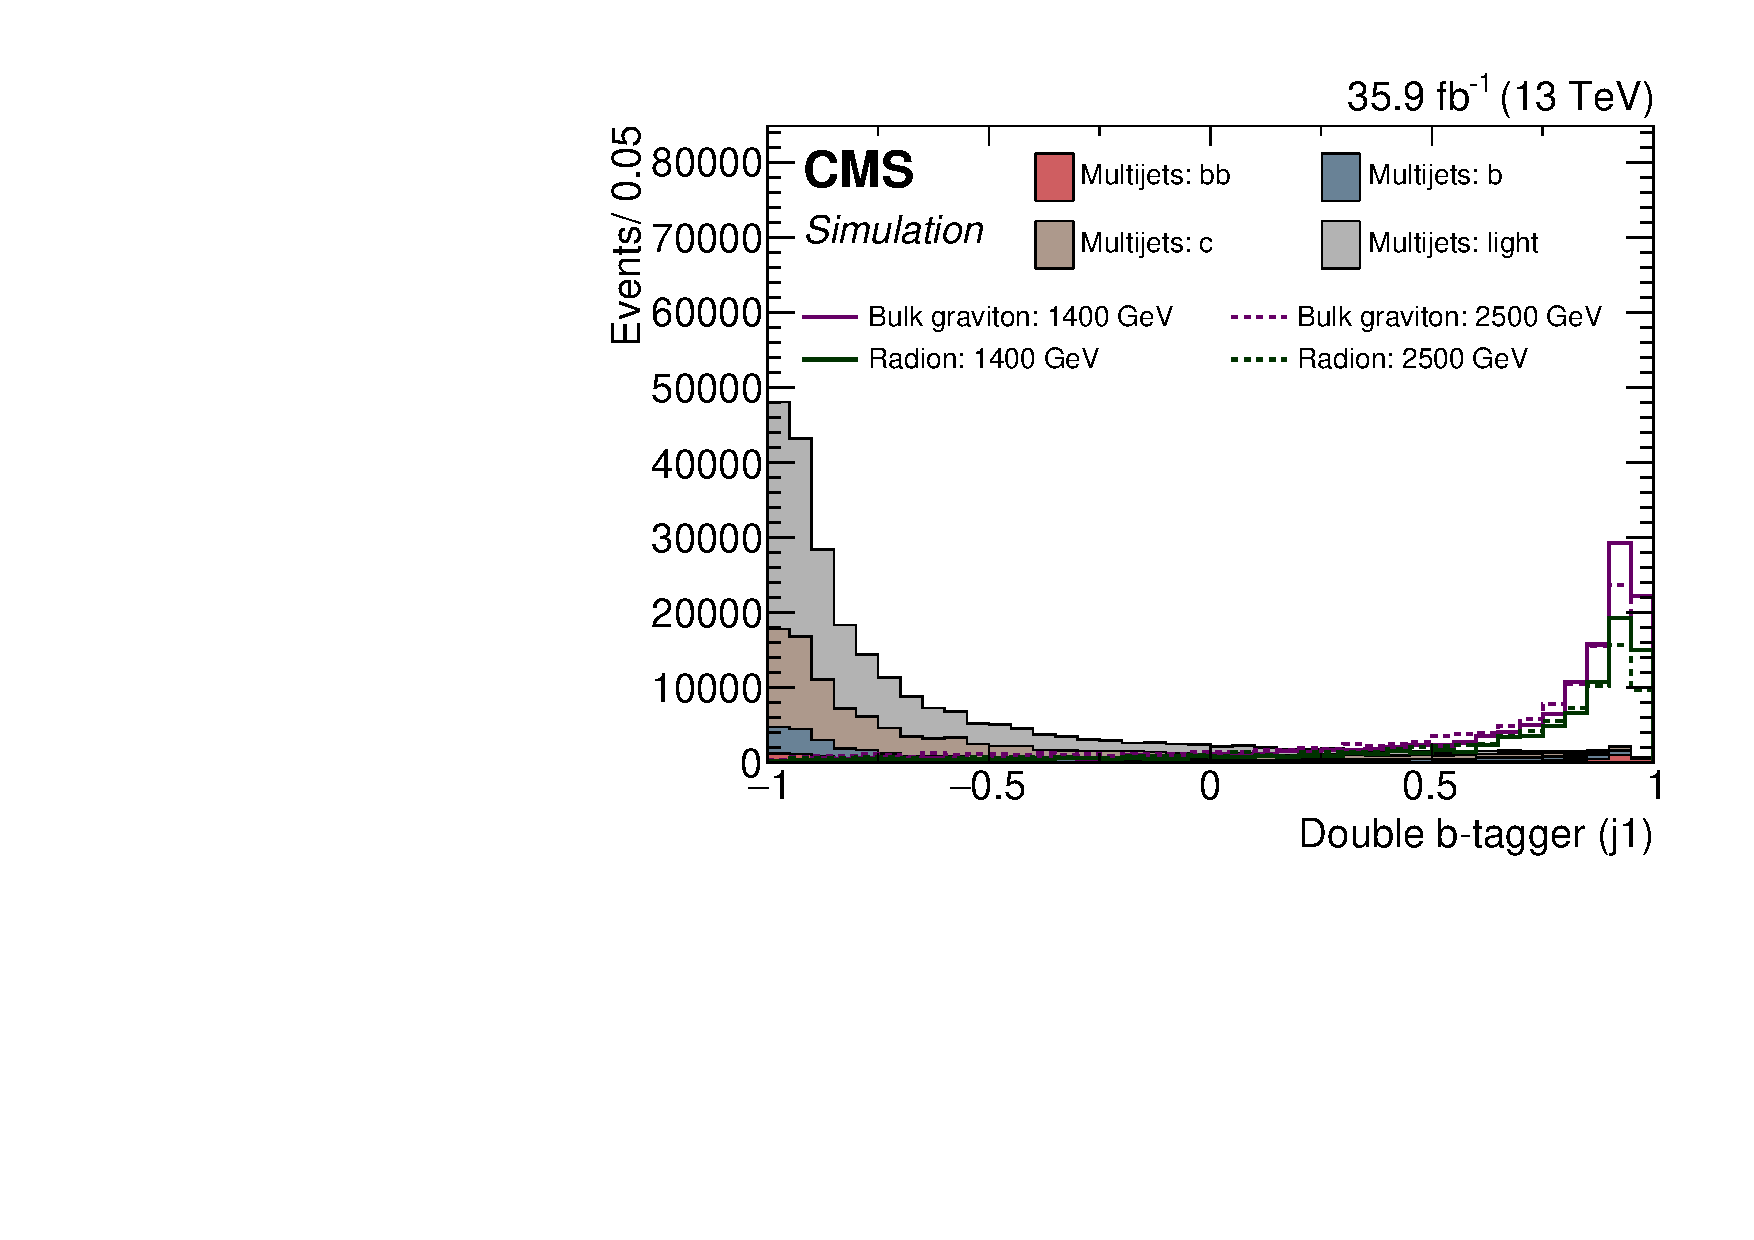
\includegraphics[width=0.45\textwidth]{Analysis/EventSelection/cmc_doubleSV_j0.pdf}
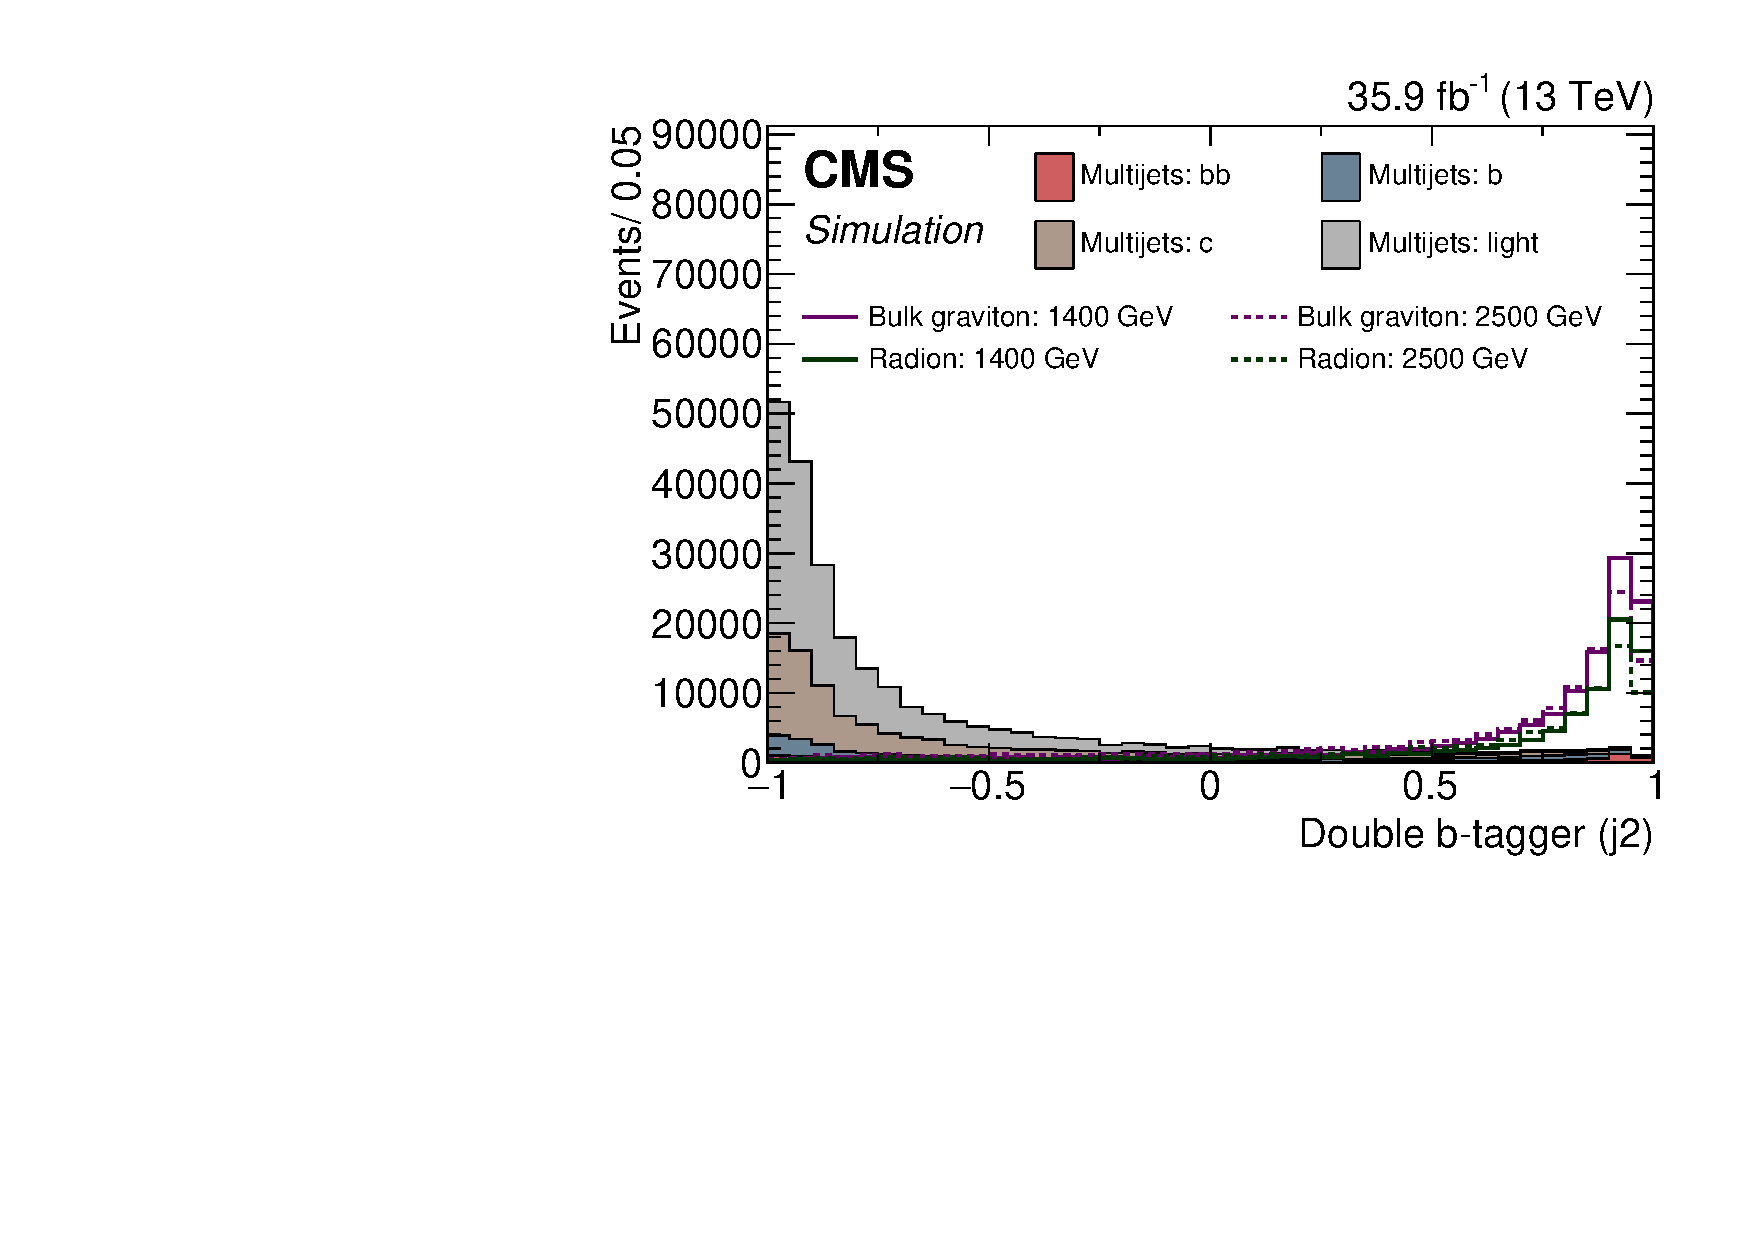
\includegraphics[width=0.45\textwidth]{Analysis/EventSelection/cmc_doubleSV_j1.pdf}
\caption{ Comparison of simulated events after the full selection excluding b-tagging, for the double b-tagger discriminant   of the leading (left) and sub-leading (right) Higgs jets. A signal cross section of 20~pb is assumed for each signal mass point. \label{fig:doublesv_prebtag}
}
\end{figure}

%The cut flow for the full event selection outlined in the previous section is given in Table~\ref{tab:BulkGravCutFlowEff} for bulk gravitons and in Table~\ref{tab:RadionCutFlowEff} for radions. The main difference in the efficiencies of the spin-2 and the spin-0 models stems from the different $\Delta\eta_{jj}$ distributions, that for the bulk graviton being more central. Therefore, the bulk gravitions have a higher efficiency than the radions.

%\subsubsection{Background Composition}

%In order to study the background composition of the events passing our selection criteria without unblinding, two different control regions have been defined. These regions are built by inverting either the $\tau_{21}$ or the double-b tag cuts for exactly one of the two selected jets.

%\noindent
%\textbf{N-subjettiness inverted control region}:
%The $\tau_{21}$ inverted control region has been selected by applying all of the event selection criteria except the $\tau_{21}$ requirement on the leading jet. Instead this jet is required to fail $tau_{21}$ requirement.
%In this comparison no SF is applied and simulation yield is scaled to match the one in data (data/MC is $\approx 1.26$) in Figures \ref{fig:jet1_tau_inverted} and \ref{fig:jet2_tau_inverted}.
%The major background from QCD multijet production is simulated and compared with the data. The multijet background has been split by flavor content.

%\begin{figure}[h!]
%\centering
%\includegraphics[width=0.45\textwidth]{Analysis/EventSelection/anti_tau21_rereco_doublebtagv4/puppiSDMassThea_j0.pdf}
%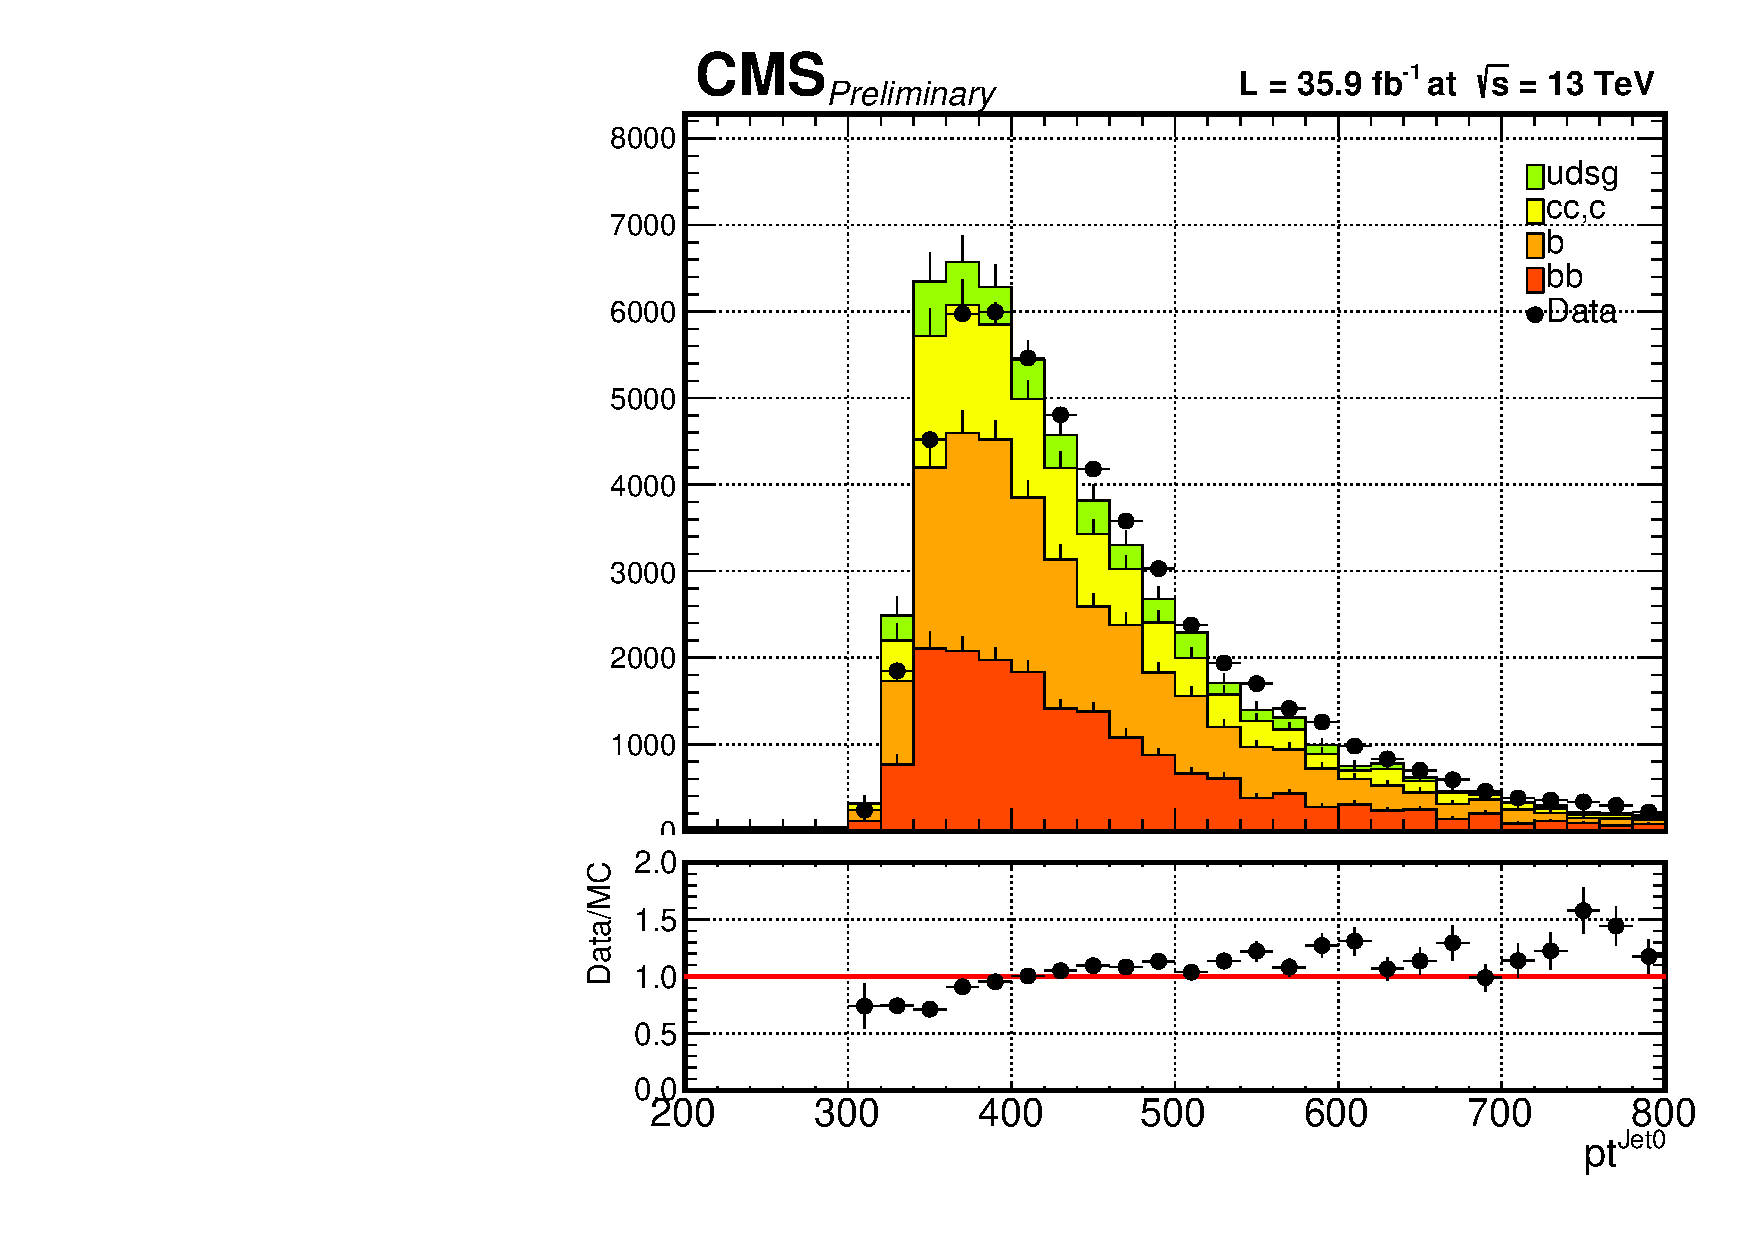
\includegraphics[width=0.45\textwidth]{Analysis/EventSelection/anti_tau21_rereco_doublebtagv4/pt_j0.pdf}
%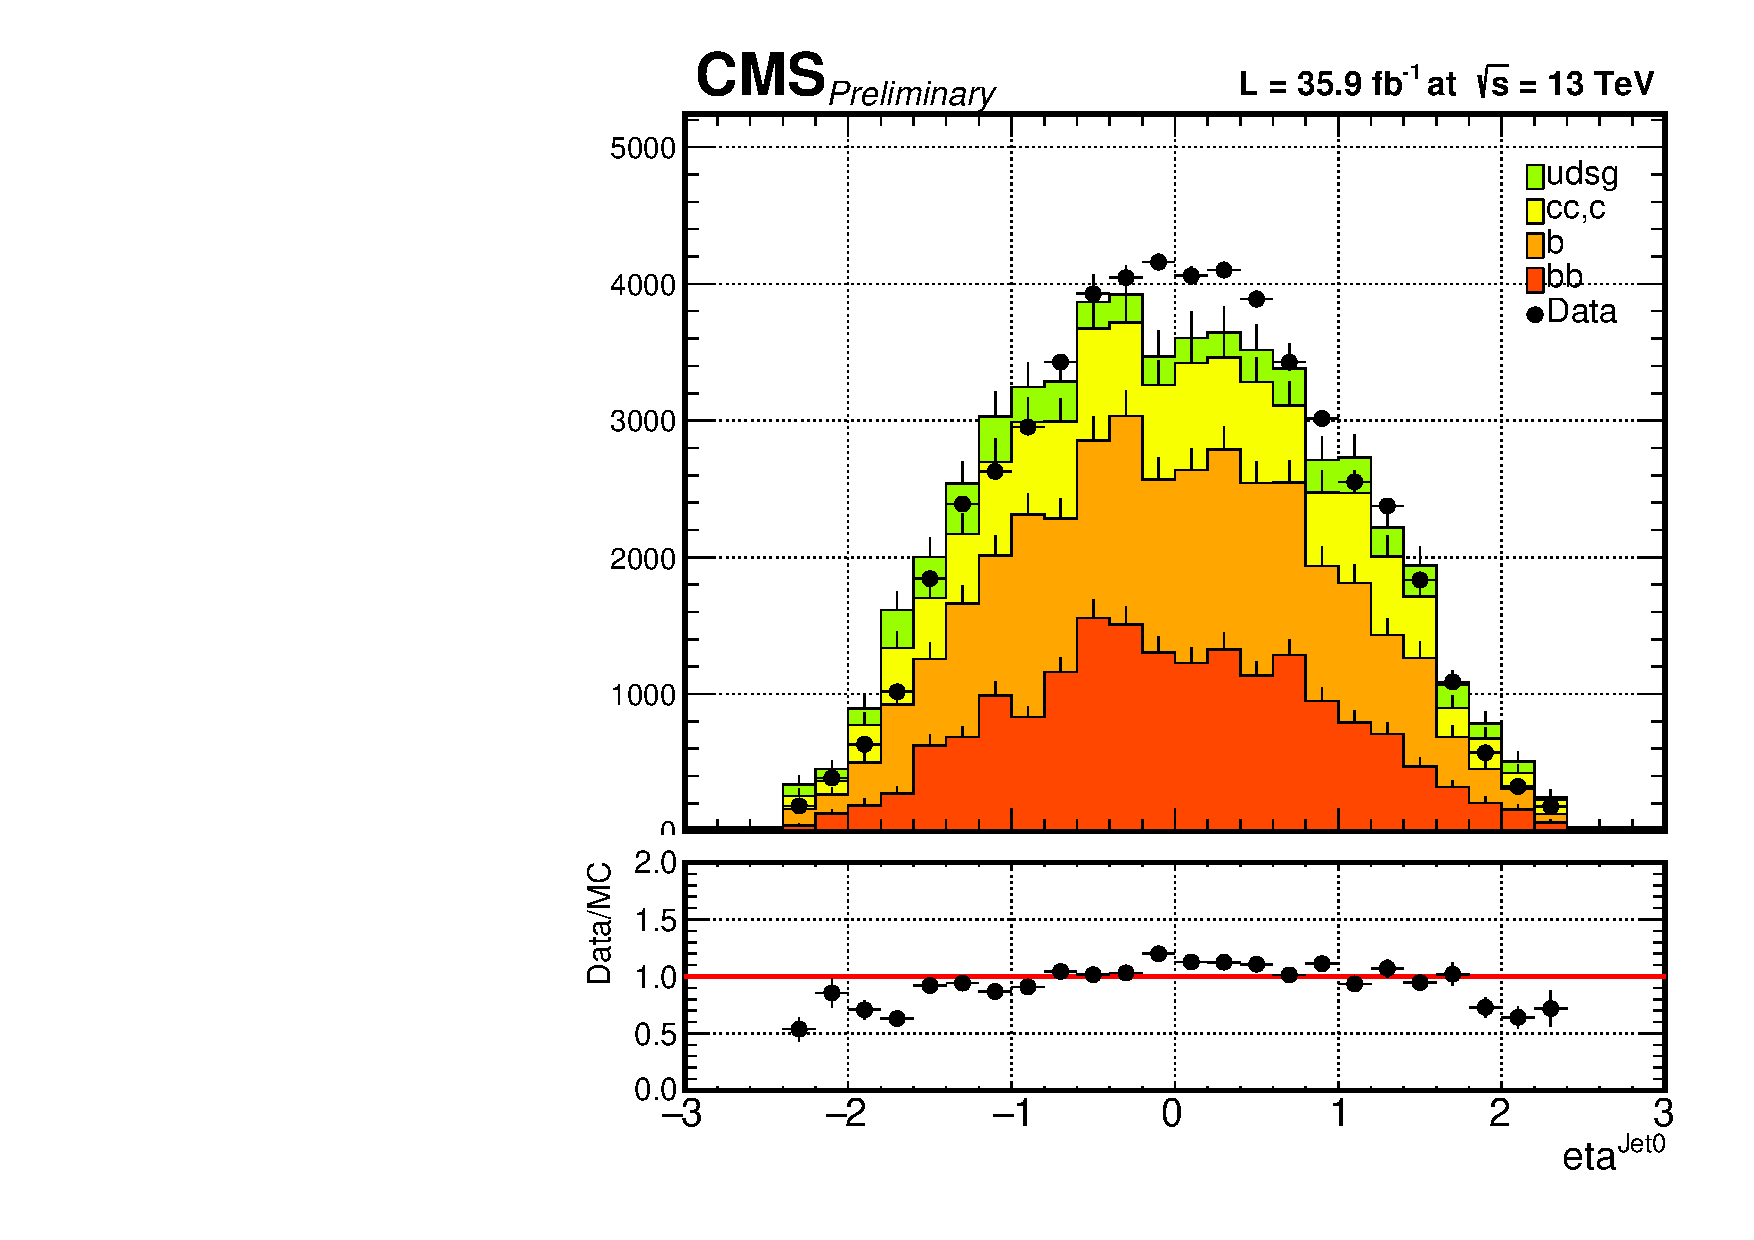
\includegraphics[width=0.45\textwidth]{Analysis/EventSelection/anti_tau21_rereco_doublebtagv4/eta_j0.pdf}
%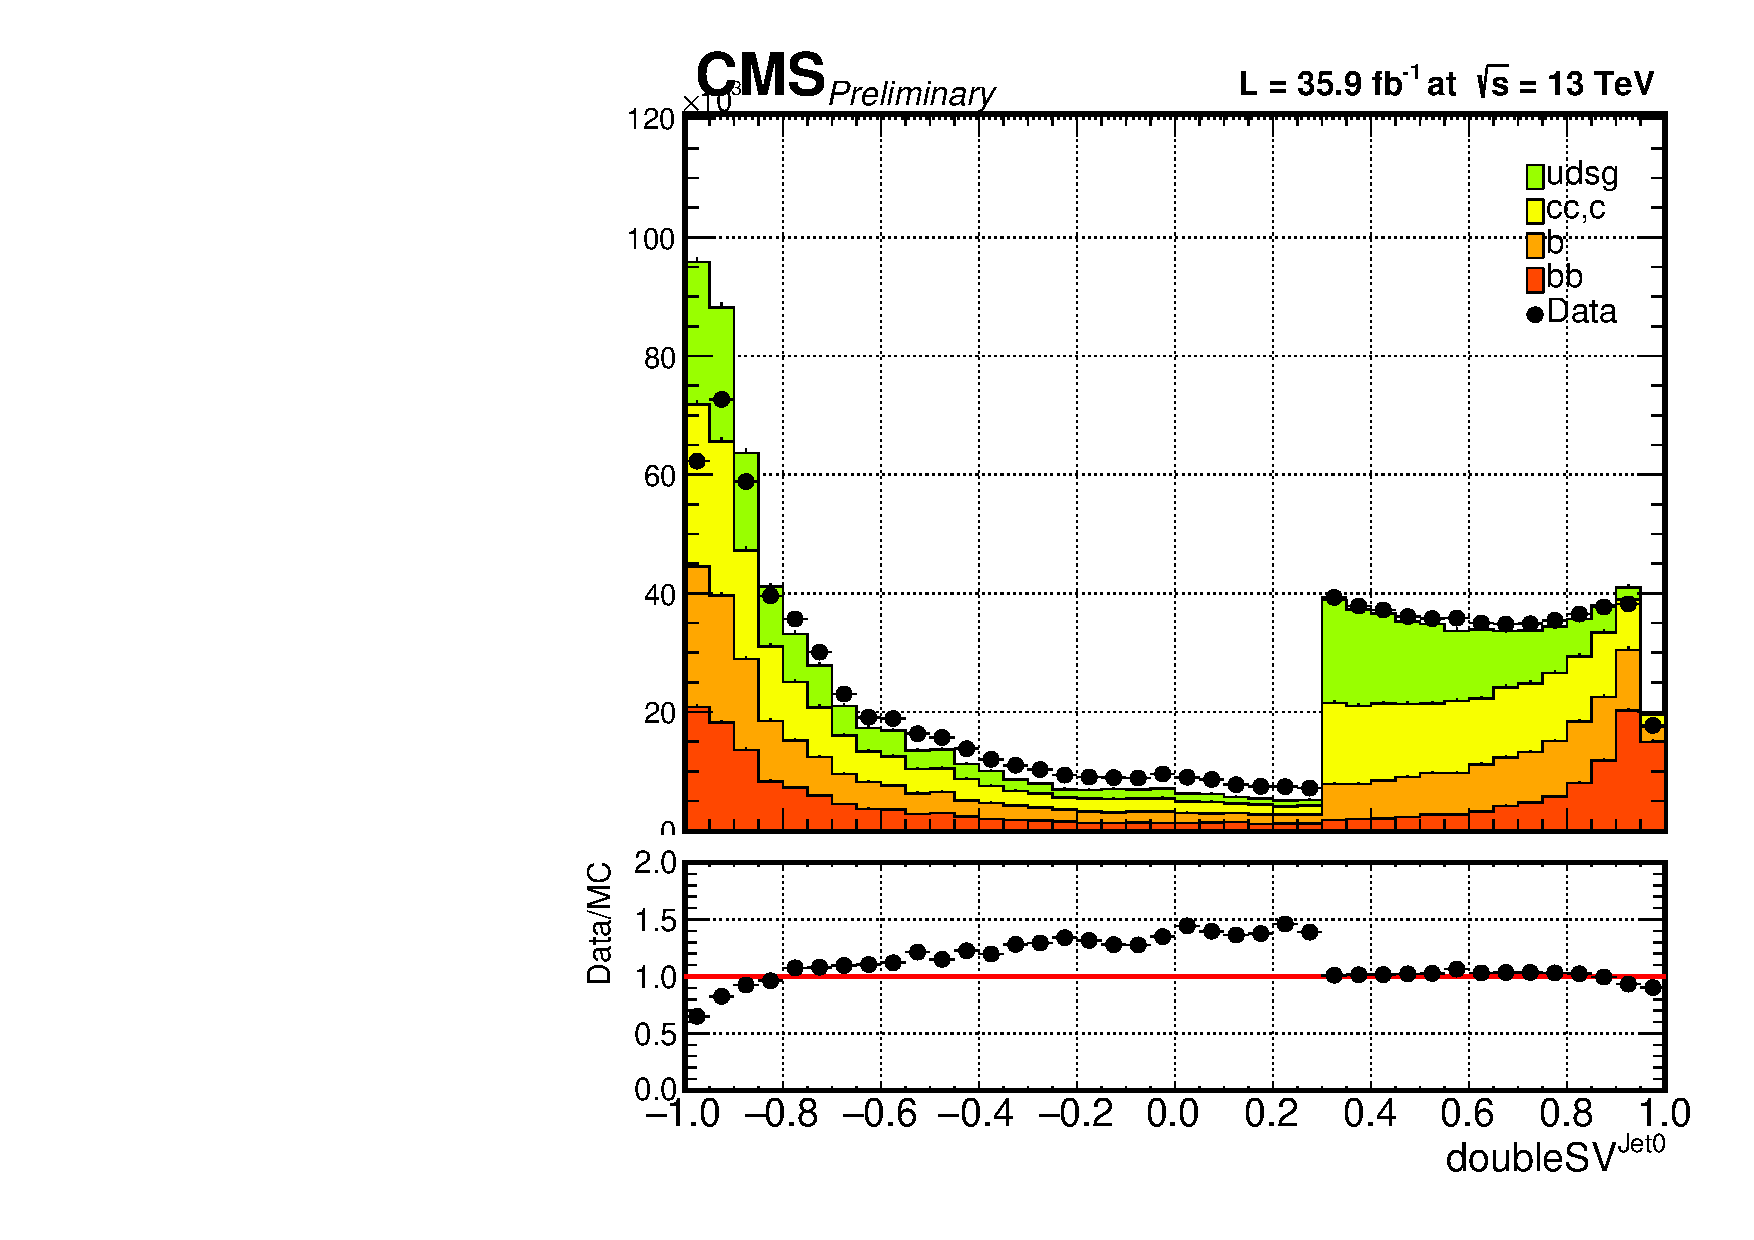
\includegraphics[width=0.45\textwidth]{Analysis/EventSelection/anti_tau21_rereco_doublebtagv4/doubleSV_j0.pdf}
%\caption{ Comparison plots of data/simulation for kinematic observables and double-b tag value for the leading jet in the $\tau_{21}$ inverted control %sample. From left to right: Thea-corrected softdrop mass, $p_{T}$, $\eta$ and double-b tag discriminator.}
%\label{fig:jet1_tau_inverted}
%\end{figure}

%\begin{figure}[h!]
%\centering
%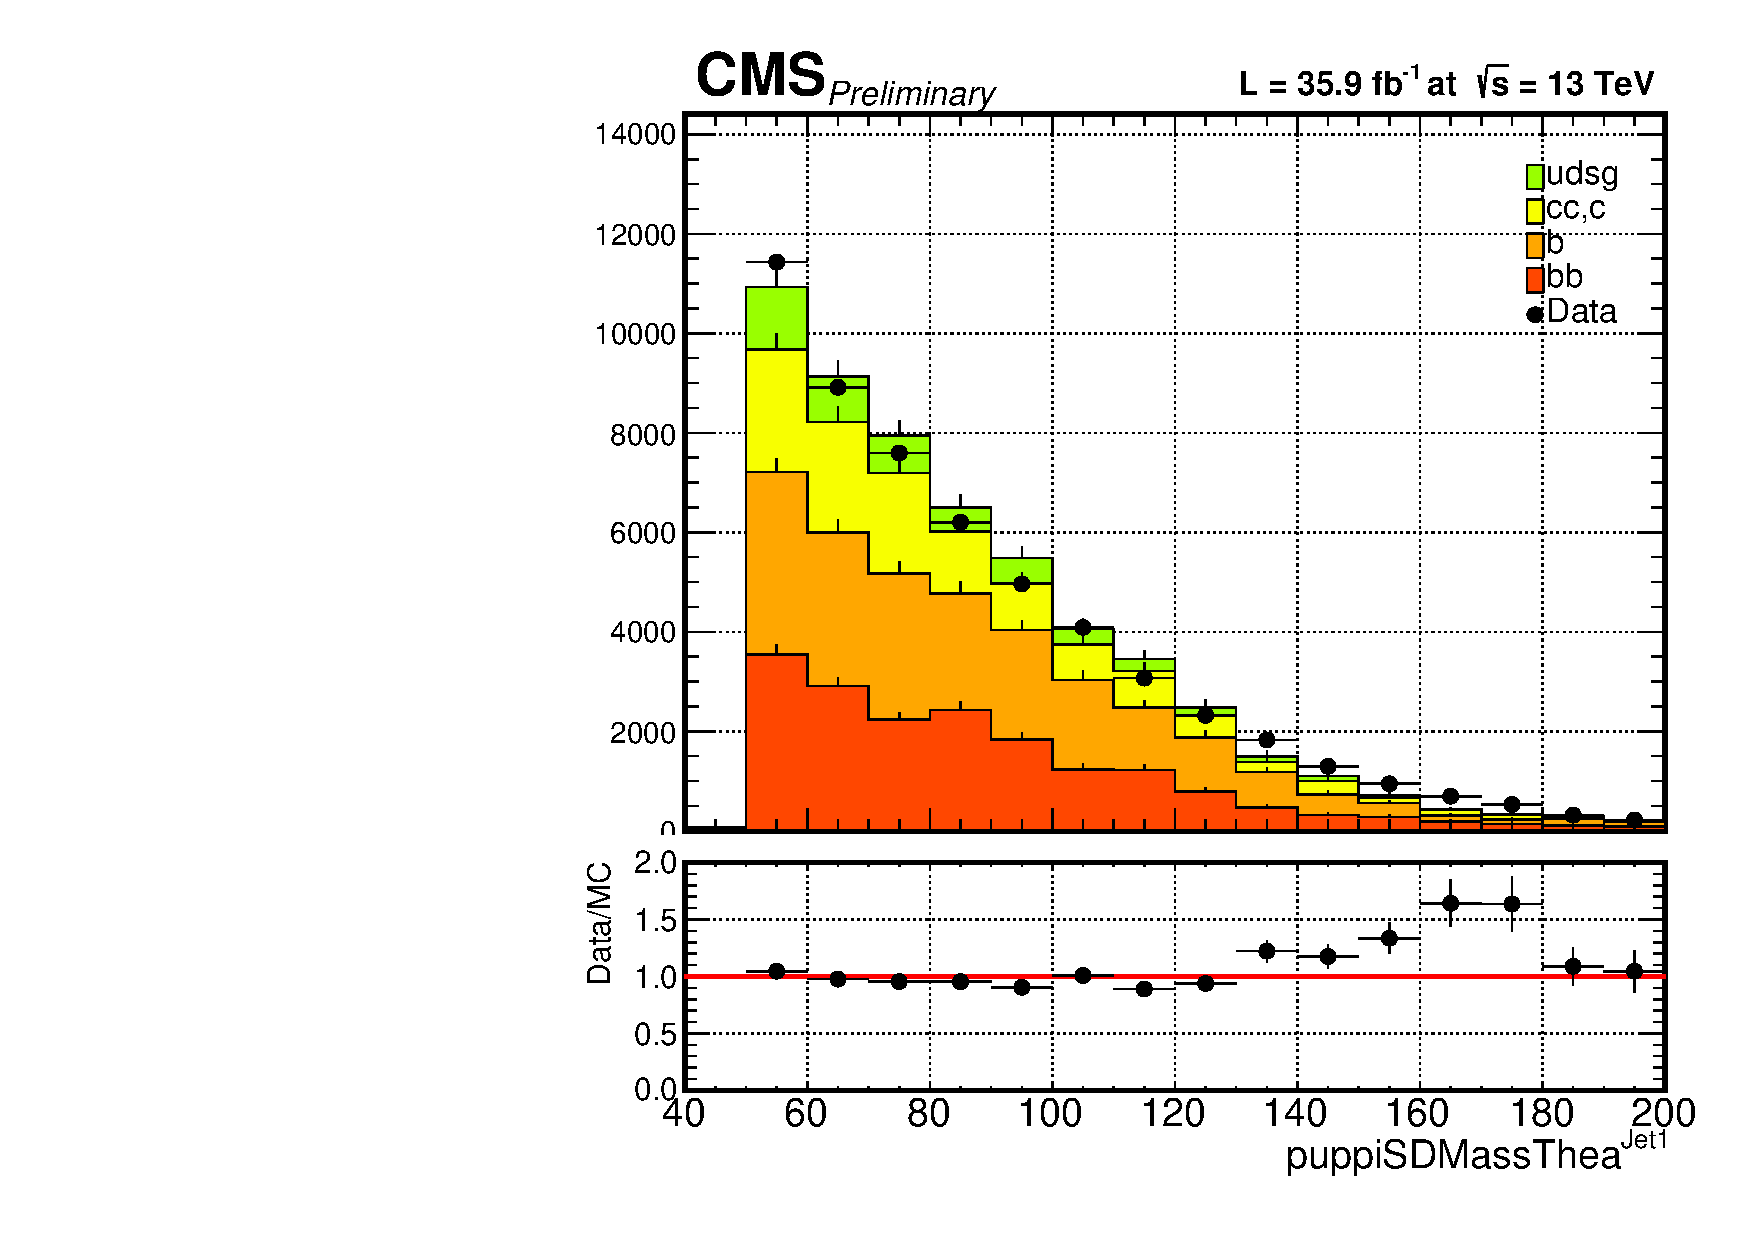
\includegraphics[width=0.45\textwidth]{Analysis/EventSelection/anti_tau21_rereco_doublebtagv4/puppiSDMassThea_j1.pdf}
%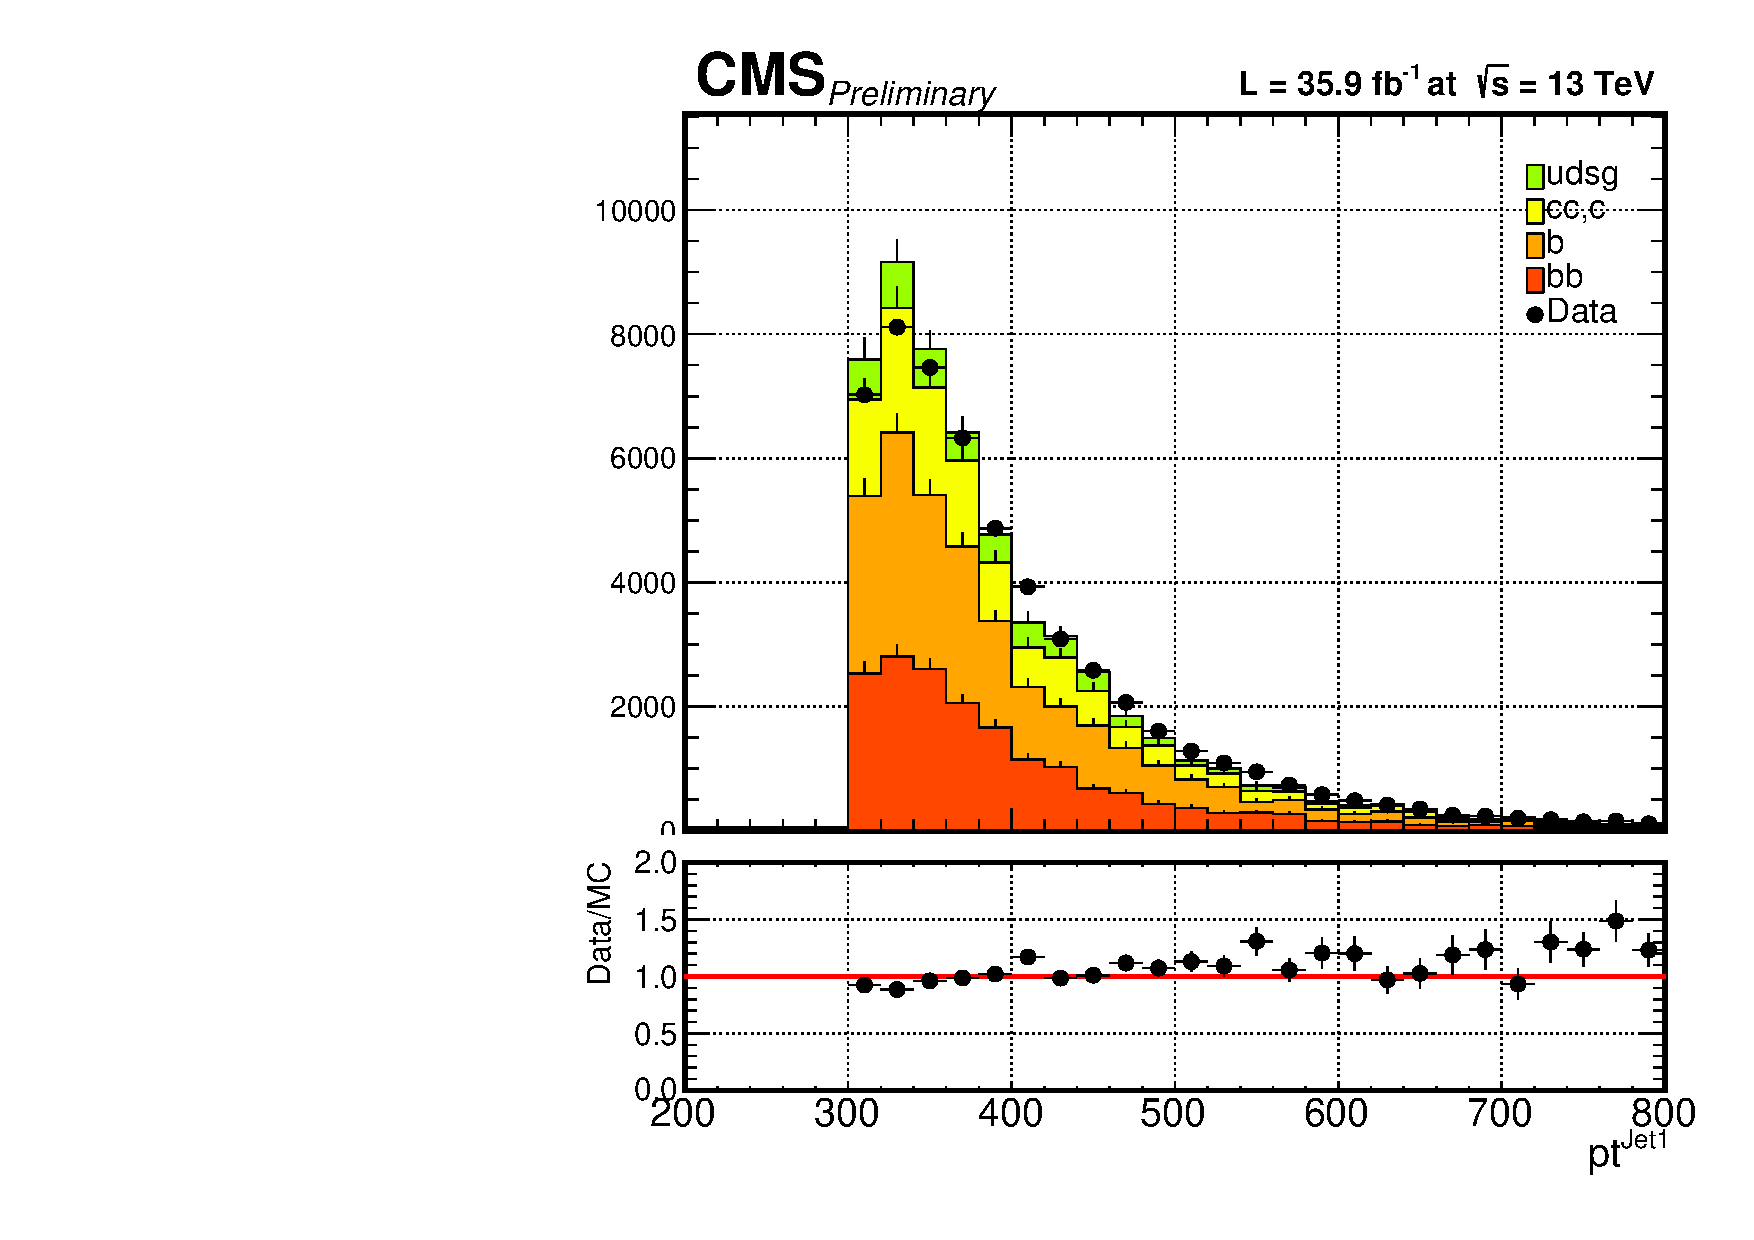
\includegraphics[width=0.45\textwidth]{Analysis/EventSelection/anti_tau21_rereco_doublebtagv4/pt_j1.pdf}
%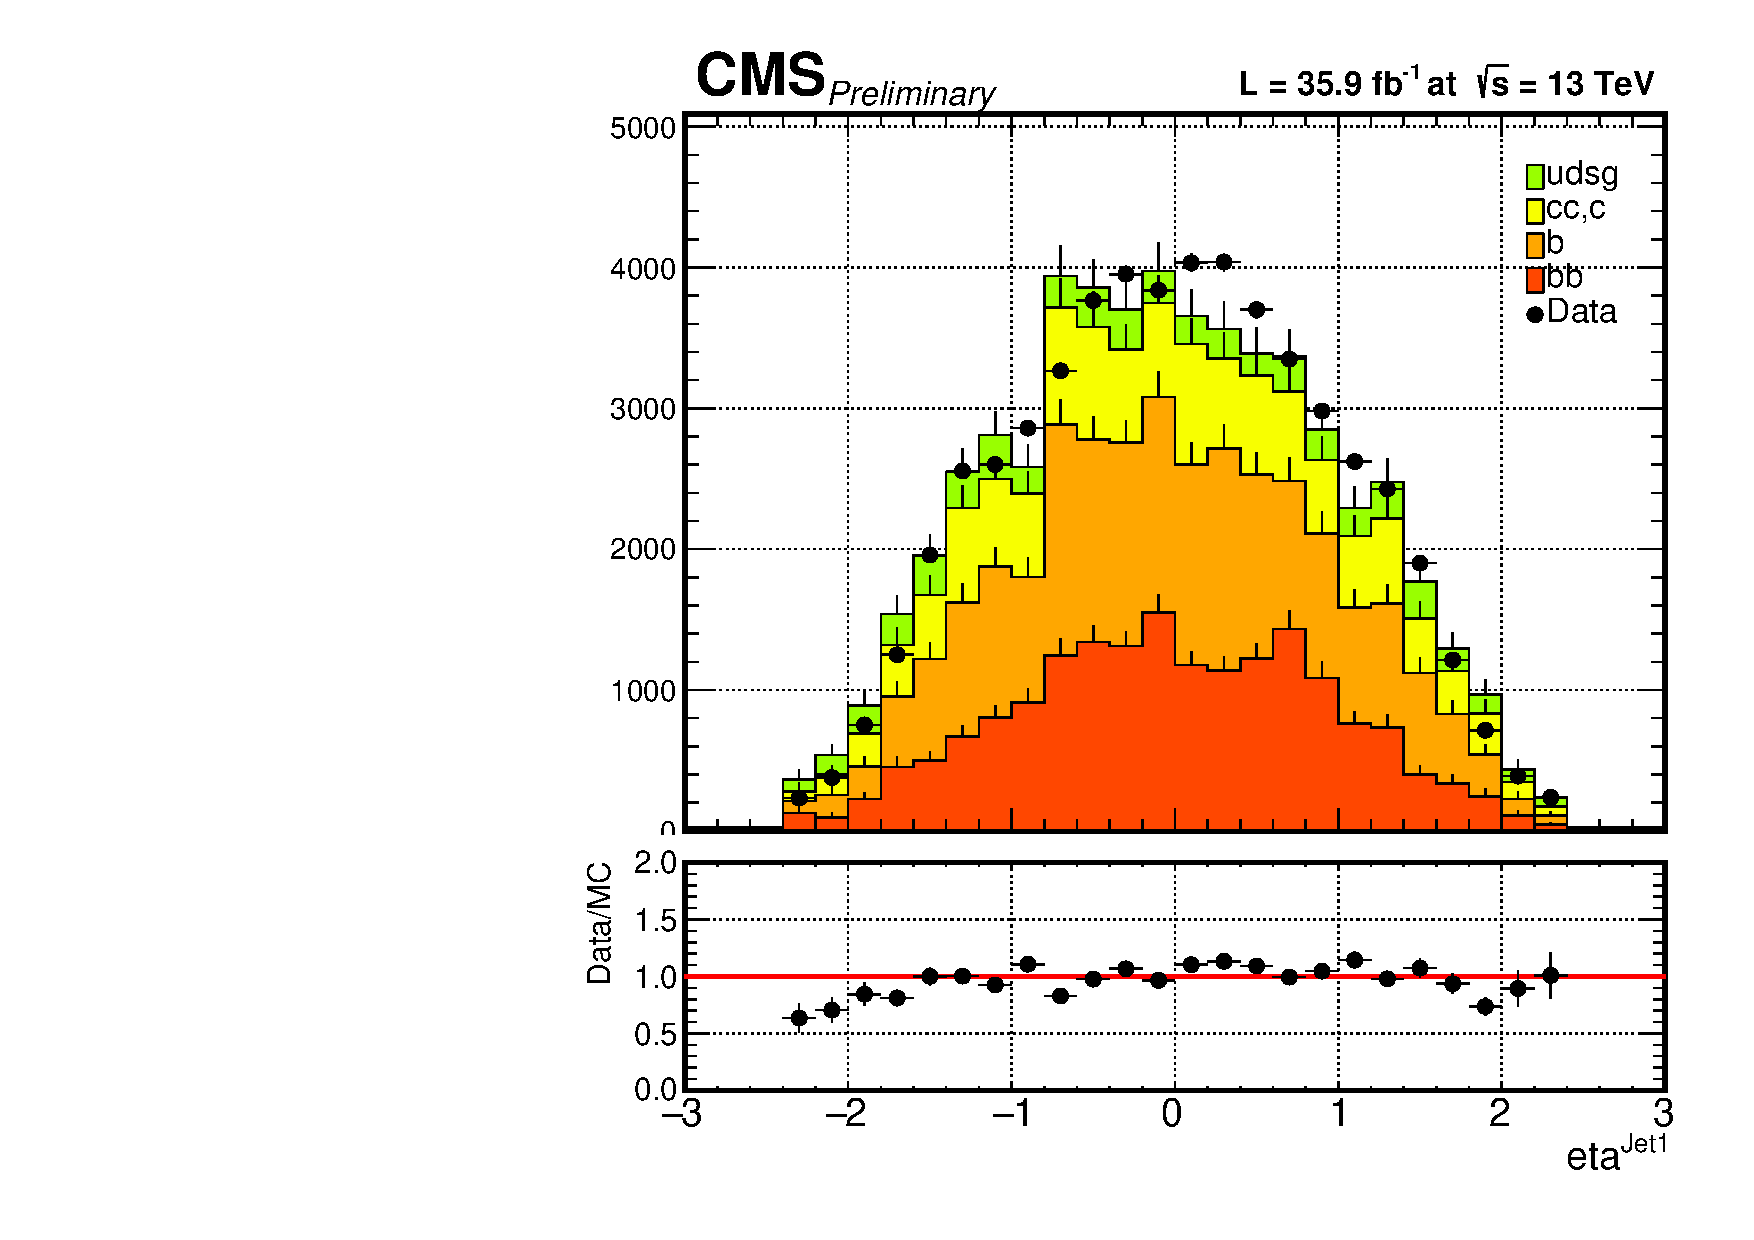
\includegraphics[width=0.45\textwidth]{Analysis/EventSelection/anti_tau21_rereco_doublebtagv4/eta_j1.pdf}
%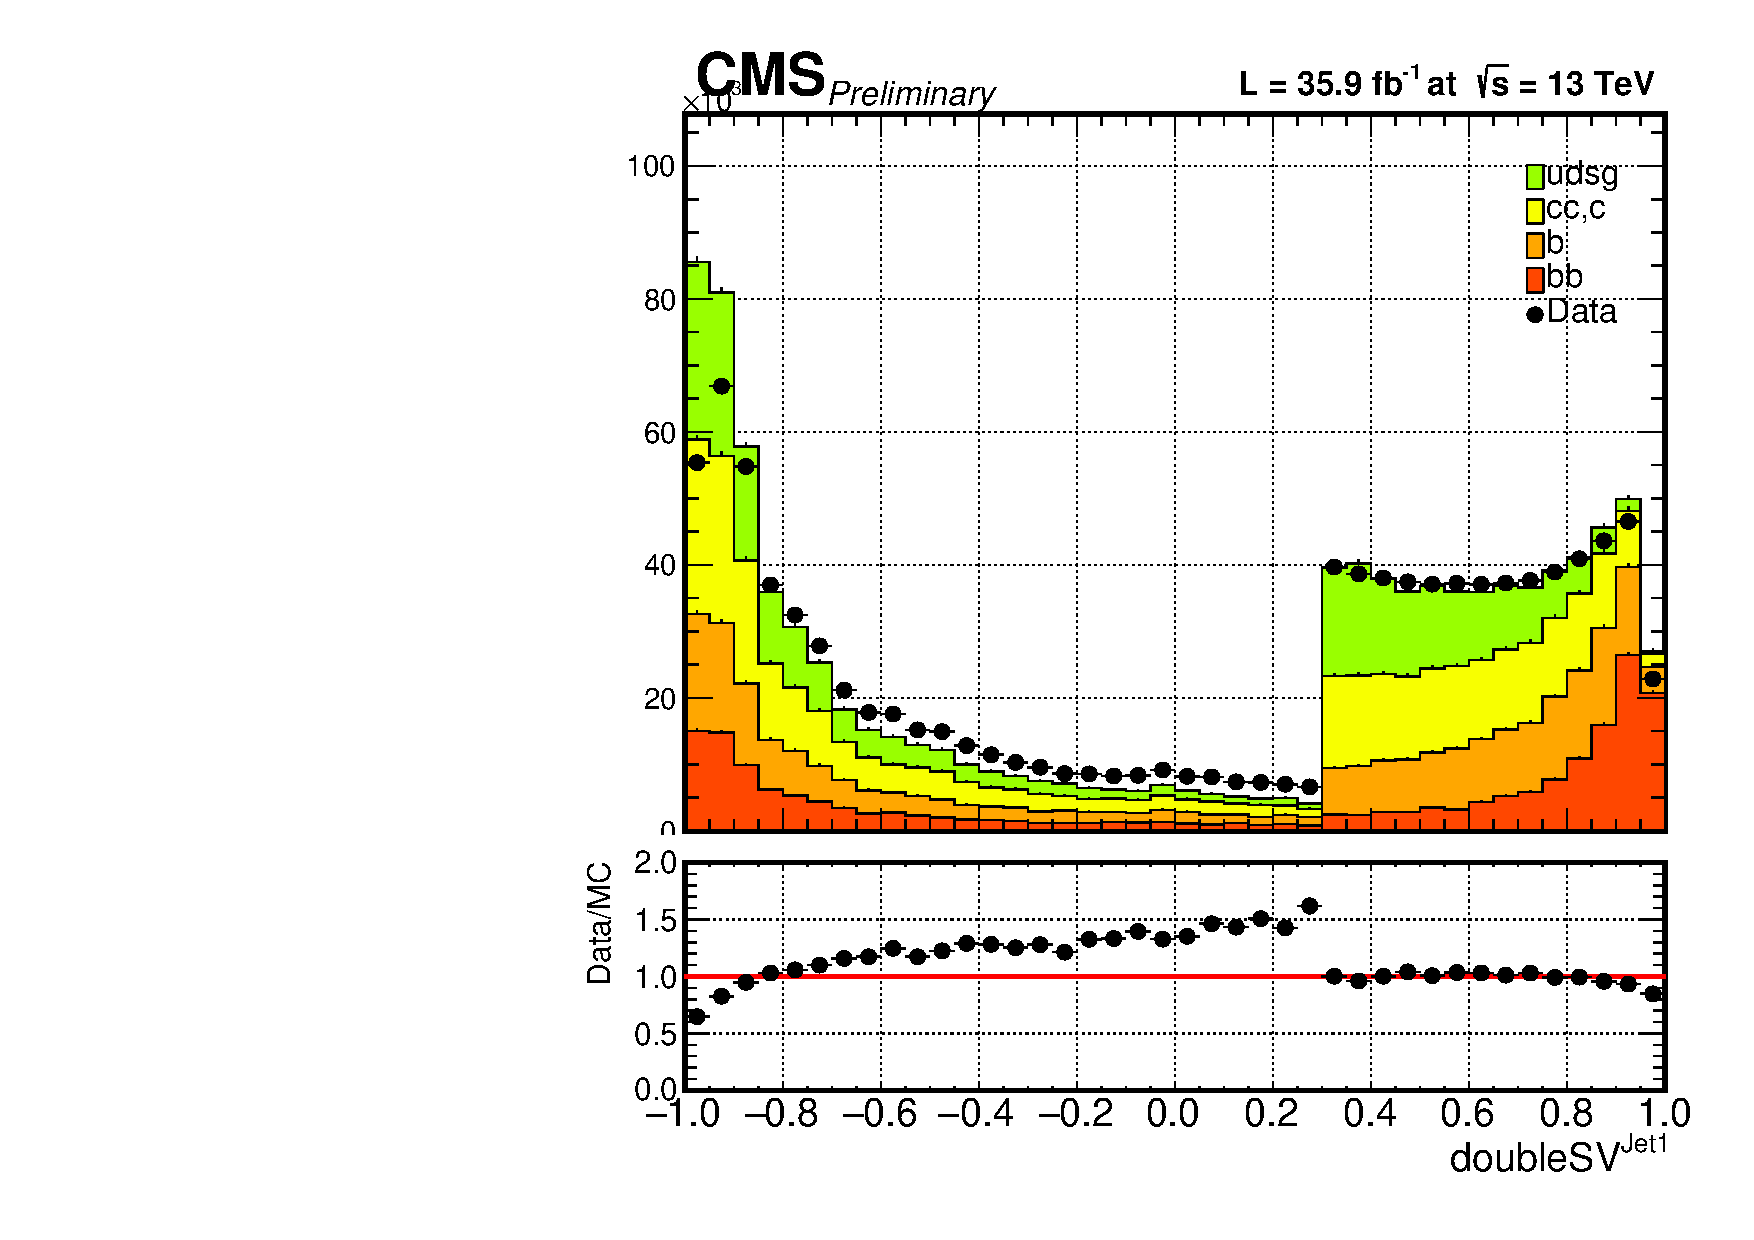
\includegraphics[width=0.45\textwidth]{Analysis/EventSelection/anti_tau21_rereco_doublebtagv4/doubleSV_j1.pdf}
%\caption{ Comparison plots of data/simulation for kinematic observables and double-b tag value for the second jet in the $\tau_{21}$ inverted control sample. From left to right: Thea-corrected softdrop mass, $p_{T}$, $\eta$ and double-b tag discriminator.}
%\label{fig:jet2_tau_inverted}
%\end{figure}


%\begin{figure}[h!]
%\centering
%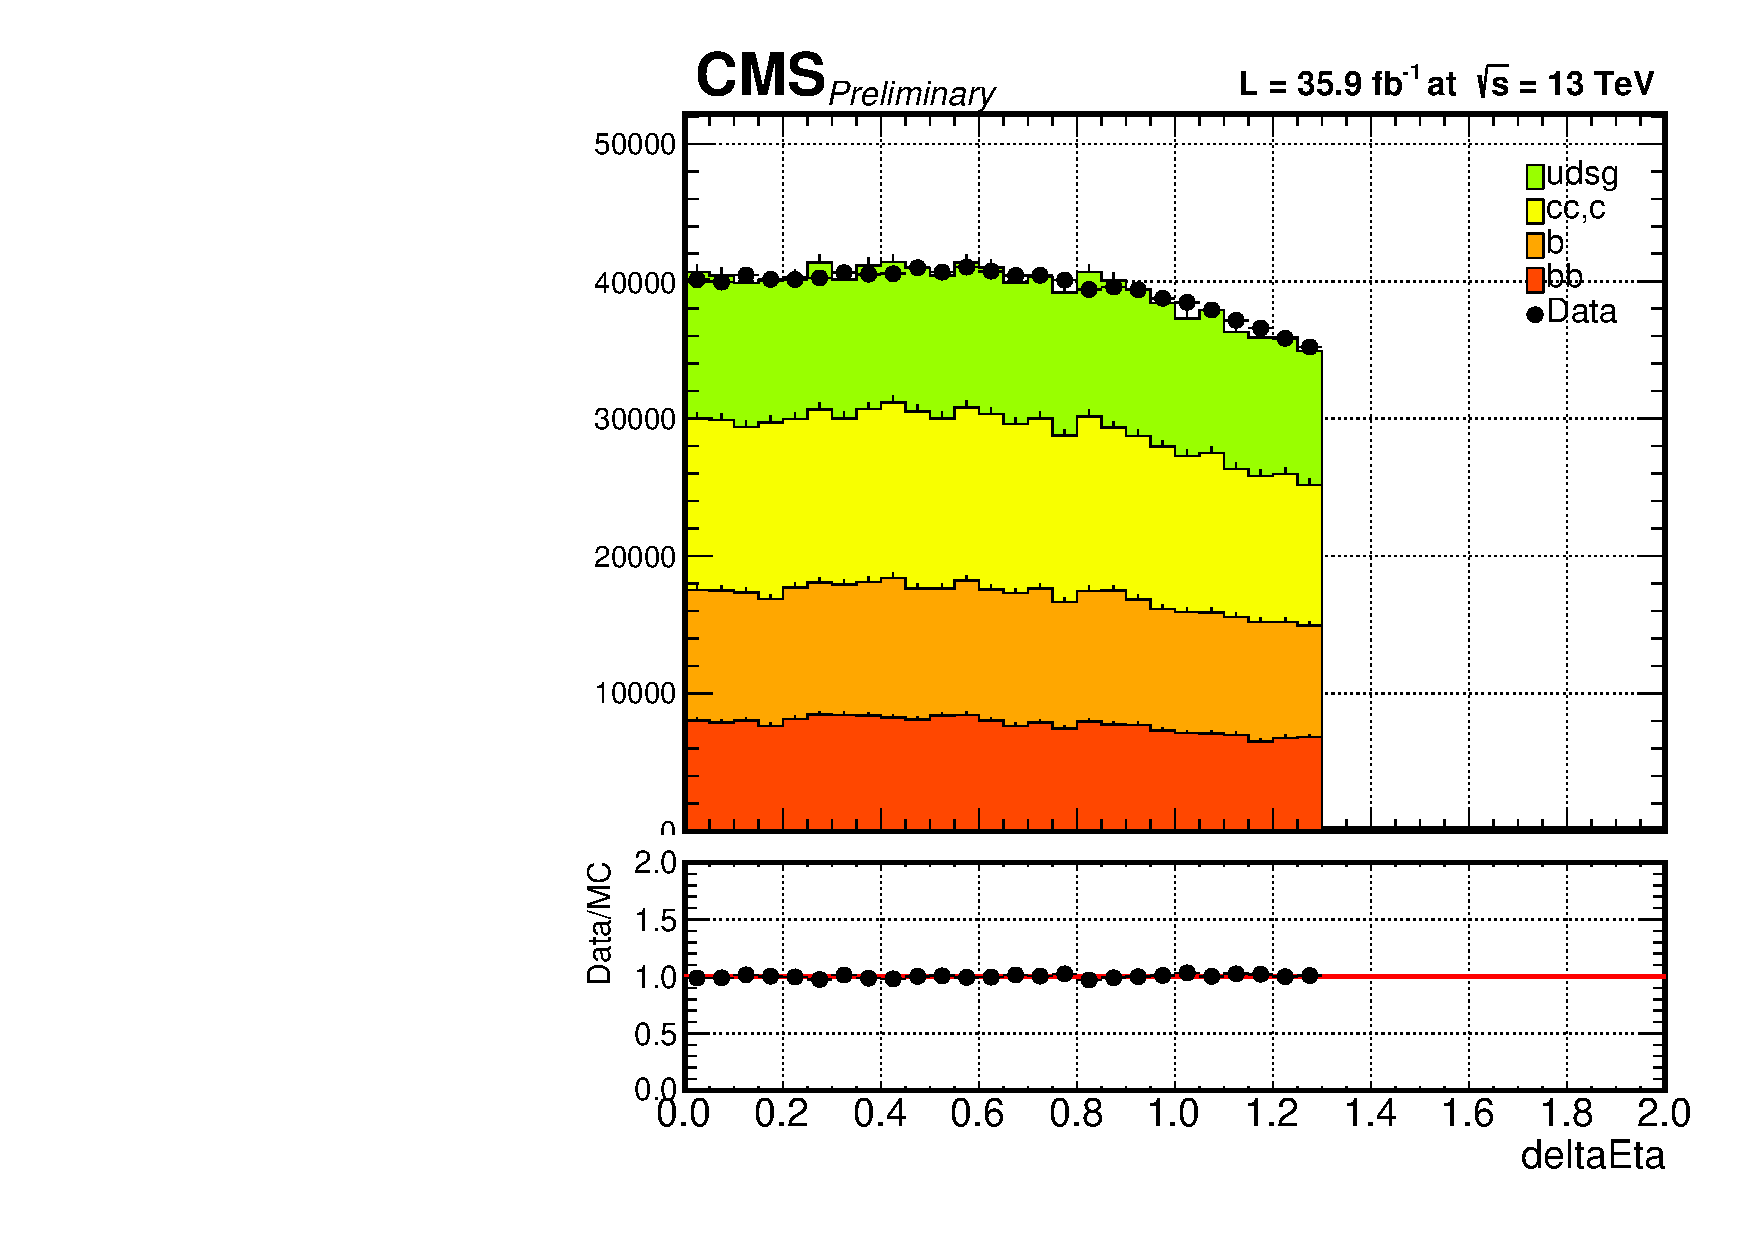
\includegraphics[width=3.5 in]{Analysis/EventSelection/anti_tau21_rereco_doublebtagv4/deltaEta.pdf}
%\caption{ Comparison plot of data/simulation for the pseudorapidity difference between the two Higgs-jet candidates $\Delta\eta_{jj}$ in the $\tau_{21}$ inverted control sample.}
%\label{fig:deta_tau_inverted}
%\end{figure}

%\noindent
%\textbf{Double-b inverted control region}:
%The double-b tag inverted control region has been selected by applying all the event selection criteria except for the double-b tag requirement on the leading jet. Instead the leading jet is required to fail the double-b tag loose requirement.
%In this comparison no SF is applied and simulation yield is scaled to match the one in data (Data/MC is $\approx 0.88$) in Figures \ref{fig:jet1_double-b_tag_inverted} and \ref{fig:jet2_double-b_tag_inverted}. The main contributing background is multi-jet production from QCD.

%\begin{figure}[h!]
%\centering
%\includegraphics[width=0.45\textwidth]{Analysis/EventSelection/anti_doublebtag_rereco_doublebtagv4/puppiSDMassThea_j0.pdf}
%\includegraphics[width=0.45\textwidth]{Analysis/EventSelection/anti_doublebtag_rereco_doublebtagv4/pt_j0.pdf}
%\includegraphics[width=0.45\textwidth]{Analysis/EventSelection/anti_doublebtag_rereco_doublebtagv4/eta_j0.pdf}
%\includegraphics[width=0.45\textwidth]{Analysis/EventSelection/anti_doublebtag_rereco_doublebtagv4/puppiTau21_j0.pdf}
%\caption{ Comparison plots of data/simulation for kinematic and substructure observables for the leading jet in the double-b tag inverted control sample. From left to right: Thea-corrected softdrop mass, $p_{T}$, $\eta$ and $\tau_{21}$.}
%\label{fig:jet1_double-b_tag_inverted}
%\end{figure}

%\begin{figure}[h!]
%\centering
%\includegraphics[width=0.45\textwidth]{Analysis/EventSelection/anti_doublebtag_rereco_doublebtagv4/puppiSDMassThea_j1.pdf}
%\includegraphics[width=0.45\textwidth]{Analysis/EventSelection/anti_doublebtag_rereco_doublebtagv4/pt_j1.pdf}
%\includegraphics[width=0.45\textwidth]{Analysis/EventSelection/anti_doublebtag_rereco_doublebtagv4/eta_j1.pdf}
%\includegraphics[width=0.45\textwidth]{Analysis/EventSelection/anti_doublebtag_rereco_doublebtagv4/puppiTau21_j1.pdf}
%\caption{ Comparison plots of data/simulation for kinematic and substructure observables for the second jet in the double-b tag inverted control sample. From left to right: Thea-corrected softdrop mass, $p_{T}$, $\eta$ and $\tau_{21}$.}
%\label{fig:jet2_double-b_tag_inverted}
%\end{figure}

%\begin{figure}[h!]
%\centering
%\includegraphics[width= 3.5 in]{Analysis/EventSelection/anti_doublebtag_rereco_doublebtagv4/deltaEta.pdf}
%\caption{ Comparison plot of data/simulation for the pseudorapidity difference between the two Higgs-jet candidates $\Delta\eta_{jj}$ in the double-b tag inverted control sample.}
%\label{fig:deta_double-b_tag_inverted}
%\end{figure}

\section{Background Estimation}
\label{sec:BkgEst}

The background is estimated in bins of the $m_{jj}^{red}$ distribution, where two different background modeling techniques are used depending on whether the resonance mass is in the $m_{jj}^{red}$ region where the triggers are fully efficient or not. Above the trigger turn-on, $m_{jj}^{red} \ge 1100$ GeV, the background is smoothly falling and therefore the shape can be modeled by a monotonically decreasing function and the ``Alphabet Assisted Bump Hunt'' (AABH) method is used. Below the trigger turn-on, $m_{jj}^{red} < 1100$ GeV, the inefficiency in the trigger causes the background to not fall smoothly and therefore an estimation is made by reweighting every event in a control region with a technique called the ``Alphabet'' method. Both of these techniques are data-driven methods which exploit a number of sidebands that are defined with respect to the soft-drop mass and the double-b tagger discriminant of the leading $p_{T}$ jet. 

Considering these two variables, a set of regions is outlined in Figure~\ref{fig:ABCDEFregions}, where the \textit{pre-tag} region is the superset of all the regions and is populated by events that pass every selection requirement except for the soft-drop mass and double-b tagger requirements on the leading jet. The \textit{signal} region is the subset of those events where the soft-drop mass of the leading jet is inside the Higgs mass window, $105-135$ GeV, and the double-b tagger discriminator is greater than 0.3 or 0.8, for the LL and TT regions, respectively. The \textit{anti-tag} region requires the leading jet double-b discriminator to be less than 0.3, with the requirement on the subleading jet either being between $0.3-0.8$ or greater than 0.8 for the LL or TT signal regions, respectively. The anti-tag regions are dominated by multijet background, as shown in Figure~\ref{fig:MCcomposition_Antitag}, and therefore can be used to predict the multijet background in the signal region. The four signal and anti-tag regions across the two categories are completely orthogonal to each other. The \textit{sideband} regions consist of events in the pre-tag region, where the the soft-drop mass of the leading jet lies outside the Higgs mass window. Based on whether the leading jet passes or fails the double-b tagger discriminator threshold, the sideband region is divided into either ``passing'' or ``failing' categories,' respectively. The definitions of the signal, the anti-tag, and the sideband regions are given in Table~\ref{tab:EventCategories}.

%The \textit{anti-tag} region is the subset of pre-tag events which pass the soft drop mass requirement but fail the double-b requirement on the leading jet. All other events in the pre-tag region constitute the leading jet mass sidebands. 

%Using these two variables, a set of regions is defined as outlined in Figure~\ref{fig:ABCDEFregions}. All of these regions together, defined as the \textit{pre-tag} region, are populated by events that pass all selection requirements except for the soft-drop mass and double-b tagger requirements on the leading jet. The \textit{signal} region is the subset of those events which pass the soft-drop mass and double-b requirements on the leading jet. The \textit{anti-tag} region is the subset of pre-tag events which pass the soft-drop mass requirement but fail the double-b requirement on the leading jet. All other events in the pre-tag region constitute the mass sidebands. 

\begin{figure}[h!]
  \centering
    \includegraphics[width=4.5 in]{Analysis/BackgroundEstimation/pretag2.pdf}
  \caption{Schematic representation of the regions used to perform the background estimate.} \label{fig:ABCDEFregions}
\end{figure}

\begin{figure}[h!]
\begin{center}
\includegraphics[width=4 in]{Analysis/EventSelection/Antitag_dijetmass_125_LogTrue.pdf}
\end{center}
\caption{The reduced invariant di-jet mass distribution in simulated QCD, $\mathrm{t\bar{t}}$, and diboson events in the combined LL and TT anti-tag region. The multijet background components for the different jet flavors are shown: events containing at least one jet with two B hadrons ($\mathrm{b\bar{b}}$) or a single one (b), events containing a jet having a charm hadron (c), and all other events (light).}
\label{fig:MCcomposition_Antitag}
\end{figure}

\begin{table}[h!]
\begin{center}
    \begin{tabular}{c c c c}
    \hline
    \hline
    Event Category &  Jet & Soft-drop mass (GeV) & Double-b tagger discriminator  \\
    \hline
    \multirow{2}{*}{Signal (LL)} & Leading & \multirow{4}{*}{$105-135$} & \multirow{2}{*}{$>0.3$, but not both $>0.8$}\\
    & Sub-leading & & \\
    \multirow{2}{*}{Signal (TT)} & Leading & & \multirow{2}{*}{$>0.8$}\\
    & Sub-leading & & \\
    \hline
    \multirow{2}{*}{Antitag (LL)} & Leading & \multirow{4}{*}{$105-135$} & $<0.3$\\
    & Sub-leading & & $0.3-0.8$\\
    \multirow{2}{*}{Antitag (TT)} & Leading & & $<0.3$\\
    & Sub-leading & & $>0.8$\\
    \hline
    \multirow{2}{*}{Sideband (LL, passing)} & Leading & $<105$ or $>135$ &  \multirow{2}{*}{$>0.3$, but not both $>0.8$}\\
    & Sub-leading & $105-135$& \\
    \multirow{2}{*}{Sideband (TT, passing)} & Leading &$<105$ or $>135$ & \multirow{2}{*}{$>0.8$}\\
    & Sub-leading & $105-135$& \\
    \hline
    \multirow{2}{*}{Sideband (LL, failing)} & Leading & $<105$ or $>135$ & $<0.3$\\
    & Sub-leading & $105-135$& $0.3-0.8$\\
    \multirow{2}{*}{Sideband (TT, failing)} & Leading &$<105$ or $>135$ & $<0.3$\\
    & Sub-leading & $105-135$& $>0.8$\\
    \hline
    \hline
    \end{tabular}
    \caption{Definition of the signal, the anti-tag, and the sideband regions used for the background estimation.}
 \label{tab:EventCategories}
\end{center}
\end{table}

\subsection{Alphabet Method}

In the absence of correlation between the soft-drop mass and the double-b tagger discriminator, the background could be estimated by measuring the ratio of the number of events passing and failing the double-b tagger selection, $R_{p/f}\equiv N_{pass}/N_{fail}$ i.e. the ``pass-fail ratio'', in a single jet mass sideband. The yield in the anti-tag region could then be scaled by $R_{p/f}$ to obtain an estimate of the background normalization in the signal region. This is a technique commonly referred to as the ``ABCD'' method. However, there is a small correlation between the double-b tagger discriminator and the soft-drop mass, which can be seen in Figure~\ref{fig:twotone2} where all events that fall in the pre-tag region are plotted, and therefore $R_{p/f}$ is measured as a function of the soft-drop mass of the leading $p_{T}$ jet. 

\begin{figure}[h!]
  \centering
    \includegraphics[width=3.5 in]{Analysis/BackgroundEstimation/bbtagvsSDMass_SR_test.pdf}
  \caption{Distribution in the pre-tag region of the leading jet double-b tagger discriminator vs soft-drop mass in QCD simulation. The red points represent the $50\%$ quantile and show that there is a slight dependence of the double-b tagger on jet mass.} \label{fig:twotone2}
\end{figure}

The $R_{p/f}$ for the LL region is measured using the ratio of the number of events in the ``LL, passing'' and ``LL, failing'' sideband regions, as defined in Table~\ref{tab:EventCategories}. Likewise, the $R_{p/f}$ for the TT region is measured using the ratio of the number of events in the ``TT, passing'' and ``TT, failing'' sideband regions. The variation of $R_{p/f}$ as a function of the leading jet mass in each soft-drop mass sideband is fitted with a quadratic function and the fit is interpolated to the Higgs mass window of the leading jet mass. An alternative fit using a third order polynomial was found to give the same interpolated value of $R_{p/f}$ in the Higgs jet mass window. Every event in the anti-tag region is scaled by the pass-fail ratio evaluated for the leading jet mass of that event, to obtain the background prediction in the signal region.

Since the background prediction in the signal region is obtained by scaling the events in the anti-tag region, the Alphabet method assumes that the shapes of the $m_{jj}^{red}$ distributions in the pass and fail regions are the same. This is verified in QCD simulation and the $m_{jj}^{red}$ distributions in the signal region and anti-tag region for both LL and TT categories can be seen in Figure~\ref{fig:Mjj_HiggsWindow}. As a further check, the $m_{jj}^{red}$ distributions in the pass and fail regions of each sideband are compared in data and shown to have similar shapes, which can be seen in Figures~\ref{fig:MjjSidebands} and~\ref{fig:MjjSidebands_2}.

\begin{figure}[h!]
\centering
\includegraphics[width=0.45\textwidth]{Analysis/BackgroundEstimation/MjjCompare_QCD_SR_LL.pdf}
\includegraphics[width=0.45\textwidth]{Analysis/BackgroundEstimation/MjjCompare_QCD_SR_TT.pdf}\\
  \caption{Distributions of $m_{jj}^{red}$ in the signal and anti-tag regions for the LL category (left) and the TT category (right). Events are from QCD simulation and the distributions are normalized to unity to show that the distributions have similar shapes.}
\label{fig:Mjj_HiggsWindow}
\end{figure}

\begin{figure}[h!]
\centering
\includegraphics[width=0.45\textwidth]{Analysis/BackgroundEstimation/MjjCompare_Data_Sideband1.pdf}
\includegraphics[width=0.45\textwidth]{Analysis/BackgroundEstimation/MjjCompare_Data_Sideband2.pdf}
\includegraphics[width=0.45\textwidth]{Analysis/BackgroundEstimation/MjjCompare_Data_Sideband3.pdf}
\includegraphics[width=0.45\textwidth]{Analysis/BackgroundEstimation/MjjCompare_Data_Sideband4.pdf}
\caption{Distributions of $m_{jj}^{red}$ in data normalized to unity in the $50-65$ GeV sideband (top left), the $65-80$ GeV sideband (top right), the $80-95$ GeV sideband (bottom left), and the $95-105$ GeV sideband (bottom right).}
\label{fig:MjjSidebands}
\end{figure}

\begin{figure}[h!]
\centering
\includegraphics[width=0.45\textwidth]{Analysis/BackgroundEstimation/MjjCompare_Data_Sideband5.pdf}
\includegraphics[width=0.45\textwidth]{Analysis/BackgroundEstimation/MjjCompare_Data_Sideband6.pdf}
\includegraphics[width=0.45\textwidth]{Analysis/BackgroundEstimation/MjjCompare_Data_Sideband7.pdf}
\caption{Distributions of $m_{jj}^{red}$ in data normalized to unity in the $135-150$ GeV sideband (top left), the $150-165$ GeV sideband (top right), and the $165-200$ GeV sideband (bottom).}
\label{fig:MjjSidebands_2}
\end{figure}

%The Alphabet method is an extension of a common background estimation technique called the ``ABCD" method. Both of these methods expect the shapes but not the normalizations of distributions of events in the signal and anti-tag regions to be the same. If there was no correlation between the soft-drop mass and the double-b tagger, the ABCD method could be used. This method only uses a single sideband to measure the ratio of passing to failing events and then scales the anti-tag region by this ratio to obtain an estimate of the signal region. As can be seen in Figure~\ref{fig:twotone2}, where the full preselection has been applied to simulated events, the double-b discriminator has a slight dependence on the soft-drop mass. Therefore, to obtain the normalization, a conversion ratio or the pass-faill ratio, $R_{p/f}$, that depends on the leading jet mass is extracted from the multiple jet mass sidebands. This is done by fitting a quadratic function to the variation of $R_{p/f}$ as a function of the leading jet mass. An alternative fit using a third order polynomial was found to give the same interpolated value of $R_{p/f}$ in the Higgs jet mass window. Every event in the antitag region is scaled by the pass-fail evaluated for the leading jet mass of that event, to obtain the background prediction in the signal region. 

%\begin{figure}[h]
%  \centering
%    \includegraphics[width=\textwidth]{Analysis/BackgroundEstimation/TwoToneBAfter.pdf}
%  \caption{Dependence of the double b-tagger on the jet mass after the preselection is applied. We separate high HT and low HT events. The solid curve represents the profile distribution of a respective region while the dashed line is the profile of the other HT region.} \label{fig:twotone2}
%\end{figure}



\subsubsection{Results in Simulation}

Prior to unblinding the data, the validity of the Alphabet method was tested on simulation. Figure~\ref{fig:QCD_Rpf} shows the quadratic fit in the mass sidebands of $R_{p/f}$ for both the LL and TT regions. Note that the pass-fail ratios in the Higgs mass window are not included in the fit and the true value of the pass-fail ratio in the Higgs mass window is shown to agree within uncertainties to the $R_{p/f}$ prediction. The estimated background after scaling the anti-tag region by the predicted $R_{p/f}$ is compared to the true background in the signal region in Figure~\ref{fig:QCD_Background}.Two systematic uncertainties arise naturally from this estimate. The dominant error comes from the statistical uncertainty in the $R_{p/f}$ fit to the mass sideband regions, which is shown as a dashed line enveloping the fit in Figure~\ref{fig:QCD_Rpf}. This error can be treated as fully correlated between all mass bins when setting limits. A smaller source of error is from propagating the statistical uncertainty in the anti-tag region to the signal region and is uncorrelated between bins.

\begin{figure}[h!]
\centering
\includegraphics[width=0.45\textwidth]{Analysis/BackgroundEstimation/HHSR_Fit_HH_LL_QCD.pdf}
\includegraphics[width=0.45\textwidth]{Analysis/BackgroundEstimation/HHSR_Fit_HH_TT_QCD.pdf}\\
  \caption{The pass-fail ratio in simulation of the leading $p_{T}$ jet for the LL (left) and TT (right) signal region categories as a function of the difference between the soft-drop mass of the leading jet and the Higgs boson mass. The measured ratio in different bins of $m_{j_{1}}-m_{H}$ is used in the fit (red solid line), except in the region around $m_{j_{1}}-m_{H}=0$, which corresponds to the signal region (blue markers). }
\label{fig:QCD_Rpf}
\end{figure}

\begin{figure}[h!]
\centering
\includegraphics[width=0.45\textwidth]{Analysis/BackgroundEstimation/HHSR_Plot_HH_LL_QCD.pdf}
\includegraphics[width=0.45\textwidth]{Analysis/BackgroundEstimation/HHSR_Plot_HH_TT_QCD.pdf}\\
  \caption{The reduced mass distributions in simulation for the LL (left) and TT (right) signal region categories. The point with bars show the actual events in the signal region, while the histogram shows the estimated background and associated uncertainty. The difference between the events and the predicted background, divided by the statistical uncertainty is shown in the lower panels.}
\label{fig:QCD_Background}
\end{figure}

To further test this method, a check was performed to verify that the estimate is free of bias when a signal is introduced. This was done by injecting a bulk graviton signal sample with bulk graviton mass at 1800 GeV and the cross section scaled to $10$ fb into the QCD MC. The Alphabet method was then performed and the results can be seen in Figure~\ref{fig:INJ}. The background estimate performs well, with the addition of this signal having no significant effect on the background estimate.

\begin{figure}[h!]
  \centering
    \includegraphics[width=4 in]{Analysis/BackgroundEstimation/HHSR_Plot_HH_LL_INJ.pdf}
  \caption{Reconstruction of QCD background in the presence of a bulk graviton signal with a cross section of 10 $fb$ and bulk graviton mass of 1800 GeV. The background estimate is not biased by the signal.} \label{fig:INJ}
\end{figure}


To ensure that the double-b tagger discriminator does not have any jet $p_{T}$ or equivalently $m_{jj}^{red}$ dependence that is not accounted for since the pass-fail ratio is only measured as function of jet mass, the dependence of the estimated $R_{p/f}$ in different di-jet mass bins was measured in simulation. This is shown in Figure~\ref{fig:INJ2}, where the Alphabet method was performed in the LL category separately on events in three different $m_{jj}^{red}$ regions: $750 < m_{jj}^{red} < 900$ GeV, $900 < m_{jj}^{red} < 1300$ GeV, and $ m_{jj}^{red} > 1300$ GeV. 

\begin{figure}[h!]
  \centering
    \includegraphics[width=3.5 in]{Analysis/BackgroundEstimation/Rpf_MjjDependence.pdf}
  \caption{The pass-fail ratio in the LL category from events in three different $m_{jj}^{red}$ bins. The predicted pass-fail ratio in the Higgs mass window between all three cases agree with their uncertainties.} \label{fig:INJ2}
\end{figure}

\subsubsection{Closure Test in Data}

As a second test of the dependence of the double-b tagger discriminator on jet $p_{T}$, the pass-fail ratio as a function of $m_{jj}^{red}$ was explicitly measured in data for the TT region. The ratio of events in the anti-tag region to events predicted in the signal region by the pass-fail ratio is shown, binned in di-jet mass, in Figure~\ref{fig:MaximeCheckII}. The plot illustrates that there is no dependence on the pass-fail ratio as a function of di-jet mass. 

\begin{figure}[h!]
  \centering
    \includegraphics[width=3.5 in]{Analysis/BackgroundEstimation/MaximeCheckIII.png}
\caption{The ratio of events in the anti-tag region to events predicted in the signal region by the transfer factor is shown, binned in $m_{jj}^{red}$. The plot illustrates that there is no dependence on the pass-fail ratio as a function of di-jet mass. } \label{fig:MaximeCheckII}
\end{figure}

As a further test of closure, the Alphabet method was run in data in a control region similar to the signal region except that the sub-leading jet is constrained to fail the double-b requirement, double-b discriminator $<0.3$. The Alphabet method is able to accurately predict the pass-fail ratios in the Higgs mass window, as well as the $m_{jj}^{red}$ distribution in the control region. Results are shown in Figure~\ref{F:closuredata} for two values of the cut on the leading jet double-b: 0.8 and 0.3.

\begin{figure}[h!]
\centering
\includegraphics[width=0.45\textwidth]{Analysis/BackgroundEstimation/HHSR_Fit_HH_TT_Data_Closure.pdf}
\includegraphics[width=0.45\textwidth]{Analysis/BackgroundEstimation/HHSR_Plot_HH_TT_Data_Closure.pdf}
%\includegraphics[width=0.45\textwidth]{Analysis/BackgroundEstimation/HHSR_Fit_M0.pdf}
%\includegraphics[width=0.45\textwidth]{Analysis/BackgroundEstimation/HHSR_Plot_M0.pdf}
\includegraphics[width=0.45\textwidth]{Analysis/BackgroundEstimation/HHSR_Fit_HH_LL_Data_Closure.pdf}
\includegraphics[width=0.45\textwidth]{Analysis/BackgroundEstimation/HHSR_Plot_HH_LL_Data_Closure.pdf}
\caption{(left) Fits in the mass sideband regions for the pass-fail ratio $R_{p/f}$ for (from top to bottom) the tight and loose working point. (right) Application of those fits to the anti-tag region to estimate the background in the control regions, compared with the true background (black markers).}
\label{F:closuredata}
\end{figure}

%The jet flavour compositions are shown in Fig.~\ref{F:JetComposition} for a region where both jets fail the double b tagger, for the antitag region, and for the signal region. It shows that the second leading jet composition is the same for the signal and the antitag regions.

%\begin{figure}[h]
%  \centering
%    \includegraphics[width=0.45\textwidth]{Analysis/BackgroundEstimation/JetComposition_2AT.pdf}
%    \includegraphics[width=0.45\textwidth]{Analysis/BackgroundEstimation/JetComposition_CR.pdf}
%    \includegraphics[width=0.45\textwidth]{Analysis/BackgroundEstimation/JetComposition_SR.pdf}
%\caption{(left) The sub-leading jet flavor in the 2 jet antitag region. (middle) The sub-leading jet flavor in the antitag region. (right) The sub-leading jet flavor in the signal region region.} \label{F:JetComposition}
%\end{figure}


\subsection{Alphabet Assisted Bump Hunt Method}

The AABH method predicts the background where $m_{jj}^{red} > 1100$ GeV and improves upon the Alphabet method by modeling the background shape as a monotonically falling function. This smooth background modeling helps reduce uncertainties in the background estimation from local statistical fluctuations in $m_{jj}^{red}$, therefore improving the signal sensitivity. The AABH method simultaneously fits a parametric model to both the anti-tag and signal region while the normalization between the two regions is constrained by the pass-fail ratio that is obtained from the sidebands in the Alphabet method. Therefore, the background is modeled as


%takes the Alphabet method and combines it with the classic bump hunt technique, where the bump hunt technique consists of interpolating a smooth shape along the $M_{jj}$ variable in the signal region and any signal would appear as a bump above the smooth fit. Since the bump hunt and Alphabet method use completely orthogonal information, the events within the Higgs mass window from bump hunt and the events within the jet mass sidebands from Alphabet, they can be combined two into a better background estimate. This is done by using the mass sidebands in the Alphabet method to obtain the $R_{p/f}$ in the Higgs mass window. A parametric model is then simultaneously fit to both the anti-tag and signal region where the relative number of background events in the two regions is constrained by $R_{p/f}$:

\begin{equation}
B(m_{jj}^{red})= R_{p/f}\times A(m_{jj}^{red}),
\end{equation}

\noindent
where $B(m_{jj}^{red})$ is the background model in the signal region and $A(m_{jj}^{red})$ is the model of anti-tag region. To account for a slight $R_{p/f}$ dependence on $m_{jj}^{red}$ at high $m_{jj}^{red}$  values (see Figure~\ref{fig:MaximeCheckII}), $R_{p/f}$ is allowed to vary linearly in $m_{jj}^{red}$ by multiplying it by the factor $(1+lin\ast m_{jj}^{red})$. The signal normalization is unconstrained in the fit, while the uncertainties in the parameters of the functions used to model the background and $R_{p/f}$ are treated as nuisance parameters. 

Three models were considered to parameterize the background shape in the signal and anti-tag region: 

\begin{itemize}
\item
Exponential (1-parameter): $N e^{-a m_{jj}^{red}}$

\item
Leveled exponential (2-parameter): $N e^{\frac{-a m_{jj}^{red}}{1+abm_{jj}^{red}}}$

\item
Quadratic levelled exponential (3-parameter): $N e^{\frac{-am_{jj}^{red}}{1+abm_{jj}^{red}}-\frac{c(m_{jj}^{red})^2}{1+bc(m_{jj}^{red})^2}}$.
\end{itemize}

\noindent
To determine which function to use a Fisher F-test~\cite{FTest} was employed. An F-test is a way to compare statistical models that have been fitted to a data set, in order to identify the model that best fits the data. It compares variances between the data and the model for two different model functions and checks if there is a real variance reduction on using an extra parameter. The $p$-values tell the probability that $n$ parameters describe the data significantly worse than $n+1$ parameters. If the $p$-value is below 0.05 it means roughly that at 95\% confidence level (CL) we need $(n+1)$ parameters. The results of the F-test indicate that a 2-parameter function is optimal for modeling the background. Therefore, the final models used are

\begin{gather}
N\ast e^{-m_{jj}^{red}\ast bgp2/(1+m_{jj}^{red}\ast bgp1\ast bgp2)}\label{eq:SignalRg},\\
N\ast R_{p/f}\ast(1+lin\ast m_{jj}^{red}) e^{-m_{jj}^{red}\ast bgp2/(1+m_{jj}^{red}\ast bgp1\ast bgp2)} \label{eq:BackgroundRg},
\end{gather}

\noindent
where Eq~\ref{eq:SignalRg} and Eq~\ref{eq:BackgroundRg} parameterize the signal and anti-tag regions, respectively. The parameters $N$, $bgp1$, and $bgp2$ are shared between the two fit functions. 

%\begin{figure}[h!]
%\begin{center}
%  \includegraphics[width=0.33\textwidth]{Analysis/BackgroundEstimation/1aLL.pdf}
%  \includegraphics[width=0.33\textwidth]{Analysis/BackgroundEstimation/1aTT.pdf}
%  \includegraphics[width=0.33\textwidth]{Analysis/BackgroundEstimation/1bLL.pdf}
%  \includegraphics[width=0.33\textwidth]{Analysis/BackgroundEstimation/1bTT.pdf}
%  \includegraphics[width=0.33\textwidth]{Analysis/BackgroundEstimation/1cLL.pdf}
%  \includegraphics[width=0.33\textwidth]{Analysis/BackgroundEstimation/1cTT.pdf}
%\end{center}
%  \caption{The 1- (top), 2-(middle), and 3-parameter (bottom) fits of the backgrounds in the anti-tag region in the data for the LL (left column) and the TT (right column) categories. It is shown that there is no appreciable change in the $\chi^{2}/NDF$ going from the 2-parameter to the 3-parameter models. Thus the 2-parameter leveled-exponential is used in the final fit.} \label{fig:app_FTest}
%\end{figure}

\subsubsection{Closure Tests}

The first validation of this method was done using QCD MC, in both the LL and TT regions. Plots of the signal and anti-tag regions with the AABH fit applied are shown in Figs.~\ref{fig:MCaabhLL} and \ref{fig:MCaabhTT}. The fits are shown with and without the linear constraint on the pass-fail ratio $R_{p/f}$ and these are consistent, showing that $R_{p/f}$ has very little dependence on $m_{jj}^{red}$. A goodness of fit (GOF) test was done using the data to confirm that the leveled exponential models the background well. The signal strength was set to zero for this fit and a p-value of 0.97 was obtained showing that the model describes the data well. 

\begin{figure}[h!]
\centering
\includegraphics[width=0.45\textwidth]{Analysis/BackgroundEstimation/CR_RooFit_Exp_log_QCD_SR_LL_pvalue.pdf}
\includegraphics[width=0.45\textwidth]{Analysis/BackgroundEstimation/CR_RooFit_Exp_log_QCD_AT_LL_pvalue.pdf}
  \caption{Fits in the LL region in the signal (left) and anti-tag (right) regions from QCD as used by the AABH approach. The fits before (pre-fit) and after the likelihood fit are shown. The pre-fit curve is obtained using only the anti-tag region.}
\label{fig:MCaabhLL}
\end{figure}

\begin{figure}[h!]
\centering
\includegraphics[width=0.45\textwidth]{Analysis/BackgroundEstimation/CR_RooFit_Exp_log_QCD_SR_TT_pvalue.pdf}
\includegraphics[width=0.45\textwidth]{Analysis/BackgroundEstimation/CR_RooFit_Exp_log_QCD_AT_TT_pvalue.pdf}
\caption{Fits in the TT region in the signal (left) and anti-tag (right) regions from QCD as used by the AABH approach. The fits before (pre-fit) and after the likelihood fit are shown. The pre-fit curve is obtained using only the anti-tag region.}
\label{fig:MCaabhTT}
\end{figure}

A bias study was conducted for the AABH method by injecting a certain number of signal events, $n_{i}$, for three different resonance mass hypothesis: 1600 GeV, 2000 GeV, and 2500 GeV. The number of events injected for each hypotheses was zero events, two events, corresponding to a ${\sim}5\sigma$ excess at $m_{X}=1.2$ TeV, and 5 events, corresponding to a ${\sim}10\sigma$ excess at $m_{X}=2$ TeV. A maximum likelihood fit was then performed to extract the signal strength and for each combination of number of injected events and mass hypothesis the observed signal strength matched. 

%A goodness of fit (GOF) test was done using the data to confirm that the leveled exponential models the background well and the result is shown in Fig.~\ref{fig:gof_data}. The negative log-likelihood distribution and the $p$-value is shown. The signal strength is set to zero for this fit. The p-value shows that the chosen background model describes the data well for both the Alphabet and the AABH methods.

%\begin{figure}[h!]
%\centering
%\includegraphics[width=0.45\textwidth]{Analysis/BackgroundEstimation/goodness-hh-fit_AABHData.pdf}
%\includegraphics[width=0.45\textwidth]{Analysis/BackgroundEstimation/goodness125AlphabetData}
%  \caption{The goodness of fit test of the background model of the AABH method (left) and the Alphabet method (right) to the data and toy Monte Carlo. The negative log-likelihood is shown for the data and the MC toys. The signal strength is set to zero.}
%\label{fig:gof_data}
%\end{figure}


\section{Signal Modelling}
\label{sec:SignalModel}

For $m_{X} > 1100$ GeV, the $m_{jj}^{red}$ distributions for the signals are modeled using the sum of a Crystal Ball function and a Gaussian, where the two function are constrained to have the same mean value. The same modeling is used in the LL and TT categories, with parameters for the Gaussian and the Crystal Ball function differing as shown in Figure~\ref{fig:sigfit}. 

\begin{figure}[h!]
\centering
\includegraphics[width=0.49\textwidth]{Analysis/BackgroundEstimation/c_Radion_LL.pdf}
\includegraphics[width=0.49\textwidth]{Analysis/BackgroundEstimation/c_Radion_TT.pdf}
\includegraphics[width=0.49\textwidth]{Analysis/BackgroundEstimation/c_BulkGrav_LL.pdf}
\includegraphics[width=0.49\textwidth]{Analysis/BackgroundEstimation/c_BulkGrav_TT.pdf}
\caption{Signal modeling for the radion (upper row) and bulk graviton (lower row) signal using the sum of a Gaussian and Crystal Ball functions. Shown are the probablity density functions (Pdfs) for the LL (left) and TT (right) categories.}
\label{fig:sigfit}
\end{figure}

\section{Systematic Uncertainties}
\label{sec:SysUnc}

The following sources of systematic uncertainty only affect the expected signal yields without causing any significant change in the signal shape. The background is unaffected by them because it is computed entirely from data, which brings different uncertainties that will be described following the signal uncertainties. All of the systematic uncertainties are summarized in Table~\ref{tab:SysUnc}.

\begin{itemize}
\item \textbf{Luminosity:} The luminosity during 2016 data taking was measured with an overall uncertainty of $2.5\%$~\cite{Lumi}.

\item \textbf{Pileup:} Simulated samples are reweighted so that their pileup distribution matches the pileup distribution in data. The uncertainty on this reweighting is estimated by varying the minimum bias cross section by $\pm4.6\%$, resulting in an uncertainty of $2\%$.

\item \textbf{Parton Distribution Functions:} The impact on the signal acceptance due to the uncertainties in the parton distribution functions (PDFs) is estimated following the PDF4LHC procedure~\cite{PDFUncertinty}, where three different PDF sets are used: CT14~\cite{CT14}, MMHT2014~\cite{MMHT}, and NNPDF3.0~\cite{NNPDF}. The PDF uncertainties are found to be between $0.1-2\%$ depending on the resonance mass.

\item \textbf{Trigger Efficiency:} To correct the difference in trigger efficiency observed between the data and simulation a scale factor that is a function of $m_{jj}^{red}$ and $|\Delta\eta(j_{1},j_{2})|$ (see Section~\ref{sec:Triggers}) is applied. For $m_{jj}^{red} > 1100$ GeV, the efficiency in data and MC is above $99\%$ and the uncertainty in the scale factor is negligible. For $m_{jj}^{red} < 1100$ GeV, the uncertainty in the scale factor is between $1\%$ and $15\%$. 

\item \textbf{Double-b Tagging:} The efficiency of the double-b tagger is measured in an enriched gluon splitting to $\mathrm{b\bar{b}}$ data sample and signal yields are corrected to match this efficiency~\cite{DoubleB}. The corresponding uncertainty is $2-5\%$ depending on the double-b tagger requirement.

\item \textbf{$\tau_{21}$ Scale Factor:} The data to simulation scale factor for the $\tau_{21}$ selection is measured using a semi-leptonic $\mathrm{t\bar{t}}$ sample of boosted hadronic W bosons and is found to be $+30/-26\%$ for the two Higgs jets combined. An additional correction factor is applied to account for the difference in the jet shower profile of $\mathrm{W}\rightarrow \mathrm{q\bar{q}}$ and $\mathrm{H}\rightarrow \mathrm{b\bar{b}}$ decays. This correction is calculated by taking the ratio of the Higgs-tagging efficiency to the W-tagging efficiency calculated in different shower generators, \textsc{pythia 8} and \textsc{herwig++}. The efficiencies are measured using different mass bulk gravition MC samples, where the bulk graviton either decays to a pair of Higgs bosons or a pair of W bosons. A double ratio of efficiencies, $R_{\textsc{herwig}}/R_{\textsc{pythia}}$, is then calculated to provide the correction factor. The double ratio provides an estimate of how different showering algorithms handle the difference between hadronically decaying Higgs and W bosons. The corresponding uncertainty from the correction factor is in the range $7-20\%$ depending on the resonance mass.

\item \textbf{Higgs Mass Tagging:} The difference in modeling in simulation compared to data of the jet mass scale and resolution is measured in a similar manner as the $\tau_{21}$ scale factor, using a semi-leptonic $\mathrm{t\bar{t}}$ sample of boosted hadronic W bosons. The scale factor for both is one, but a $1\%$ and $20\%$ uncertainty per jet is associated with each scale factor for the jet mass scale and resolution, respectively.

\item \textbf{Jet Energy Scale:} An uncertainty on the jet energy scale is applied to the signal acceptance, according to the CMS JetMET POG. The uncertainty causes a $2\%$ fluctuation to the signal yield.

\item \textbf{Jet Energy Resolution:} An uncertainty on the jet energy resolution is applied to the signal acceptance, according to the CMS JetMET POG. The uncertainty causes a $2\%$ fluctuation to the signal yield.

\end{itemize}

The remaining uncertainties impact the multijet background estimate and depend on which background estimation method is used.

\begin{itemize}

\item \textbf{Alphabet:} For $m_{jj}^{red} < 1100$ GeV, the main source of uncertainty is due to the statistical uncertainty in the fit to the $R_{p/f}$ ratio performed in the leading Higgs jet mass sidebands. This uncertainty is fully correlated between all $m_{jj}^{red}$ bins of a particular estimate and amounts to $2.6-6.8\%$. An additional statistical uncertainty in the anti-tag region is propagated to the signal region when the estimate is made. This uncertainty is uncorrelated from bin to bin. The Barlow-Beeston Lite method~\cite{Barlow} is used to treat the bin-by-bin statistical uncertainty. These uncertainties affect both the shape of the background and the total background yield.

\item \textbf{AABH:} For $m_{jj}^{red} > 1100$ GeV, the uncertainty from the AABH background estimate is simply the uncertainty in the simultaneous fit of the anti-tag and signal regions. The dependence of $R_{p/f}$ on $m_{jj}^{red}$ is accounted for by providing a Gaussian constraint on this dependence. However, this was found to be negligible.

\end{itemize}

\begin{table}[h!]
\begin{center}
    \begin{tabular}{l c}
    \hline
    \hline
    Source &  Uncertainty($\%$) \\
    \hline
    \multicolumn{2}{c}{Signal Yield}\\
    Trigger efficiency & $1-15$\\
    H jet energy scale & 2 \\
    H jet energy resolution & 2 \\
    H jet mass scale & 1 \\
    H jet mass resolution & 20 \\
    H jet $\tau_{21}$ selection & $+30/-26$ \\
    H-tagging correction factor & $7-20$\\
    Double-b tagger & $2-5$ \\
    Pileup modeling & 2 \\
    PDFs & $0.1-2$ \\
    Luminosity & 2.5 \\
    \multicolumn{2}{c}{Background Yield}\\
    $R_{p/f}$ fit & $2.6-6.8$ \\
    \hline
    \hline
    \end{tabular}
    \caption{Summary of systematic uncertainties in the signal and background yields. \label{tab:SysUnc}}
\end{center}
\end{table}


\section{Results}
\label{sec:Results}

The quadratic fit in the leading jet $p_{T}$ sidebands of the pass-fail ratio for the LL and TT regions in data is shown in Figure~\ref{fig:AlphaRpf}. The predicted $R_{p/f}$ has good agreement with the measured $R_{p/f}$ in the Higgs mass window. The background prediction from the Alphabet method for both regions, along with the number of observed events in the signal region is shown in Figure~\ref{fig:Alpha}. A representative signal of a bulk graviton of mass 1000 GeV is overlaid for comparison. Figures~\ref{fig:AABH_AT} and~\ref{fig:AABH_SR} present the results of the AABH method's simultaneous fits to both the anti-tag and signal regions in both the LL and TT categories. In these figures the expected distribution from bulk gravitons of masses 1600 and 2500 GeV are overlaid in the signal regions. The fit to the background in the AABH method is extended just beyond the last observed event in the four fitted regions which occurs in the anti-tag region in the LL category, which is at 2838 GeV. As the parametric model is only reliable within the range of observed events, the likelihood is only evaluated up to $m_{jj}^{red} = 3000$ GeV. This results in a truncation of the signal distribution for resonances having $m_{X}$ of 2800 GeV and above, with the signal efficiency losses increasing to $30\%$ for $m_{X}=3000$ GeV, as shown in Figure~\ref{fig:sigfit}.

Over the whole mass range searched, $750-3000$ GeV, the data and the estimated backgrounds agree within uncertainties and therefore the results are interpreted in terms of upper limits on the product of the production cross sections and the branching fractions, $\sigma(\mathrm{pp}\rightarrow \mathrm{X})B(\mathrm{X}\rightarrow\mathrm{HH}\rightarrow\mathrm{b\bar{b}b\bar{b}})$, for bulk graviton and radion of various mass hypothesis.

\begin{figure}[h!]
\centering
\includegraphics[width=0.45\textwidth]{Analysis/Results/Figure_005-a.pdf}
\includegraphics[width=0.45\textwidth]{Analysis/Results/Figure_005-b.pdf}
\caption{The pass-fail ratio $R_{p/f}$ of the leading $p_{T}$ jet for the LL (left) and TT (right) signal region categories as a function of the difference between the soft-drop mass of the leading jet and the Higgs boson mass, $m_{j1}-m_{H}$. The measured ratio in different bins of $m_{j_{1}}-m_{H}$  is used in the fit (red solid line), except in the region around $m_{j_{1}}-m_{H}=0$, which corresponds to the signal region (blue triangular markers). The horizontal bars on the data points indicate the bin widths.}
\label{fig:AlphaRpf}
\end{figure}

\begin{figure}[h!]
\centering
\includegraphics[width=0.45\textwidth]{Analysis/Results/Figure_006-a.pdf}
\includegraphics[width=0.45\textwidth]{Analysis/Results/Figure_006-b.pdf}
\caption{The reduced mass distributions $m_{jj}^{red}$ for the LL (left) and TT (right) signal region categories. The points with bars show data, the histogram with a shaded band shows estimated background and associated uncertainty. The signal predictions for a bulk graviton of mass 1000 GeV, are overlaid for comparison, assuming a production cross section of 10 fb. The last bins of the distributions contain all events with $m_{jj}^{red} > 3000$ GeV. The difference between the data and the predicted background, divided by the data statistical uncertainty are shown in the lower panels.}
\label{fig:Alpha}
\end{figure}

\begin{figure}[h!]
\centering
\includegraphics[width=0.45\textwidth]{Analysis/Results/Figure_007-a.pdf}
\includegraphics[width=0.45\textwidth]{Analysis/Results/Figure_007-b.pdf}
\caption{The $m_{jj}^{red}$ distributions in the anti-tag region for the LL (left) and TT (right) categories. The black markers are the data while the curves show the pre-fit and post-fit background shapes. The difference between the data and the predicted background, divided by the data statistical uncertainty are shown in the lower panels.}
\label{fig:AABH_AT}
\end{figure}

\begin{figure}[h!]
\centering
\includegraphics[width=0.45\textwidth]{Analysis/Results/Figure_008-a.pdf}
\includegraphics[width=0.45\textwidth]{Analysis/Results/Figure_008-b.pdf}
\caption{The $m_{jj}^{red}$ distributions in the signal region for the LL (left) and TT (right) categories. The black markers are the data while the curves show the pre-fit and post-fit background shapes. The contributions of bulk gravitons of masses 1600 and 2500 GeV are shown assuming a production cross section of 10 fb. The difference between the data and the predicted background, divided by the data statistical uncertainty are shown in the lower panels.}
\label{fig:AABH_SR}
\end{figure}

The asymptotic approximation of the modified frequentist approach for confidence levels, taking the profile likelihood as a test statistic~\cite{CLs,CLs2,CLs3}, is used to compute the limit at $95\%$ confidence. The systematic uncertainties are represented as nuisance parameters in the likelihood and profiled by maximizing the likelihood with respect to the nuisances and obtaining them in terms of the parameter of interest, which is the signal strength. The LL and TT categories are combined by correlating the nuisance parameters that they share. The limits from the combination are shown in Figure~\ref{fig:Limits} and Table~\ref{tab:limits} for a narrow width radion and a bulk graviton produced through gluon-gluon fusion and assumed to decay to a pair of Higgs bosons with a branching fraction of $23\%$ and $10\%$, respectively. The expected limit on the bulk graviton is more stringent than those on the radion due to the $|\Delta\eta(j_{1},j_{2})| < 1.3$ requirement. The bulk gravitons, being spin-2 particles, produce more central jets, and hence have higher efficiency with respect to this selection criteria, than the radions. Thus, the signal sensitivity for a bulk graviton is higher than that for a radion of the same mass.

The upper limits on the production cross sections and branching fraction lies in the range $126-1.4$ fb for a narrow resonance $X$ of mass $750 < m_{X} < 3000$ GeV. Assuming $\Lambda_{R}= 3$ TeV, a radion with a mass between 970 and 1400 GeV is excluded at $95\%$ confidence level, except in a small region close to 1200 GeV, where the observed limit is 11.4 pb, the theoretical prediction being 11.2 pb. 

\begin{figure}[h!]
\centering
\includegraphics[width=0.45\textwidth]{Analysis/Results/Figure_009-a.pdf}
\includegraphics[width=0.45\textwidth]{Analysis/Results/Figure_009-b.pdf}
\caption{The limits for the spin-0 radion (left) and the spin-2 bulk graviton (right) models. The result for $m_{X}<1100$ GeV uses the background predicted by the Alphabet method, while for $m_{X}\ge 1100$ GeV the background is derived from the AABH method. The predicted theoretical cross sections for a narrow radion or a bulk graviton are also shown.}
\label{fig:Limits}
\end{figure}

\begin{table}[h!]
  \begin{center}
    \begin{tabular}{c|c|c|c|c}
      \hline\hline
      Resonance Mass & \multicolumn{2}{c|}{Radion} & \multicolumn{2}{c}{Bulk graviton} \\ \cline{2-5}
      (GeV)          & Expected & Observed & Expected & Observed \\
      \hline\hline
      750  & 81.6 & 125.9 & 50.2 & 79.4\\
      800  & 46.4 & 90.4  & 29.9 & 59.9\\
      900  & 29.8 & 44.0  & 19.5 & 29.0\\
      1000 & 20.4 & 14.2  & 13.4 & 9.3 \\
      1200 & 10.4 & 11.4  & 6.9  & 7.6 \\
      1400 & 6.3  & 6.0   & 4.4  & 4.3 \\
      1600 & 4.7  & 5.5   & 3.2  & 3.8 \\
      1800 & 3.8  & 3.8   & 2.4  & 2.4 \\
      2000 & 3.0  & 3.5   & 2.0  & 2.4 \\
      2500 & 2.0  & 1.7   & 1.4  & 1.4 \\
      3000 & 2.5  & 1.4   & 1.7  & 1.1 \\
      \hline\hline
    \end{tabular}
    \caption{Comparison of expected and observed limits on the production cross section of a resonance decaying to $\mathrm{HH}$ for the bulk graviton and the radion signal hypotheses, for different values of the resonance mass. The limits for masses below 1200 GeV are obtained using the Alphabet background estimation method, while those above use the AABH method.}\label{tab:limits}
  \end{center}
\end{table}


































